% Options for packages loaded elsewhere
\PassOptionsToPackage{unicode}{hyperref}
\PassOptionsToPackage{hyphens}{url}
\PassOptionsToPackage{dvipsnames,svgnames,x11names}{xcolor}
%
\documentclass[
  letterpaper,
  DIV=11,
  oneside]{scrreprt}

\usepackage{amsmath,amssymb}
\usepackage{lmodern}
\usepackage{iftex}
\ifPDFTeX
  \usepackage[T1]{fontenc}
  \usepackage[utf8]{inputenc}
  \usepackage{textcomp} % provide euro and other symbols
\else % if luatex or xetex
  \usepackage{unicode-math}
  \defaultfontfeatures{Scale=MatchLowercase}
  \defaultfontfeatures[\rmfamily]{Ligatures=TeX,Scale=1}
\fi
% Use upquote if available, for straight quotes in verbatim environments
\IfFileExists{upquote.sty}{\usepackage{upquote}}{}
\IfFileExists{microtype.sty}{% use microtype if available
  \usepackage[]{microtype}
  \UseMicrotypeSet[protrusion]{basicmath} % disable protrusion for tt fonts
}{}
\makeatletter
\@ifundefined{KOMAClassName}{% if non-KOMA class
  \IfFileExists{parskip.sty}{%
    \usepackage{parskip}
  }{% else
    \setlength{\parindent}{0pt}
    \setlength{\parskip}{6pt plus 2pt minus 1pt}}
}{% if KOMA class
  \KOMAoptions{parskip=half}}
\makeatother
\usepackage{xcolor}
\usepackage[left=1in,marginparwidth=2.0666666666667in,textwidth=4.1333333333333in,marginparsep=0.3in]{geometry}
\setlength{\emergencystretch}{3em} % prevent overfull lines
\setcounter{secnumdepth}{3}
% Make \paragraph and \subparagraph free-standing
\ifx\paragraph\undefined\else
  \let\oldparagraph\paragraph
  \renewcommand{\paragraph}[1]{\oldparagraph{#1}\mbox{}}
\fi
\ifx\subparagraph\undefined\else
  \let\oldsubparagraph\subparagraph
  \renewcommand{\subparagraph}[1]{\oldsubparagraph{#1}\mbox{}}
\fi

\usepackage{color}
\usepackage{fancyvrb}
\newcommand{\VerbBar}{|}
\newcommand{\VERB}{\Verb[commandchars=\\\{\}]}
\DefineVerbatimEnvironment{Highlighting}{Verbatim}{commandchars=\\\{\}}
% Add ',fontsize=\small' for more characters per line
\usepackage{framed}
\definecolor{shadecolor}{RGB}{241,243,245}
\newenvironment{Shaded}{\begin{snugshade}}{\end{snugshade}}
\newcommand{\AlertTok}[1]{\textcolor[rgb]{0.68,0.00,0.00}{#1}}
\newcommand{\AnnotationTok}[1]{\textcolor[rgb]{0.37,0.37,0.37}{#1}}
\newcommand{\AttributeTok}[1]{\textcolor[rgb]{0.40,0.45,0.13}{#1}}
\newcommand{\BaseNTok}[1]{\textcolor[rgb]{0.68,0.00,0.00}{#1}}
\newcommand{\BuiltInTok}[1]{\textcolor[rgb]{0.00,0.23,0.31}{#1}}
\newcommand{\CharTok}[1]{\textcolor[rgb]{0.13,0.47,0.30}{#1}}
\newcommand{\CommentTok}[1]{\textcolor[rgb]{0.37,0.37,0.37}{#1}}
\newcommand{\CommentVarTok}[1]{\textcolor[rgb]{0.37,0.37,0.37}{\textit{#1}}}
\newcommand{\ConstantTok}[1]{\textcolor[rgb]{0.56,0.35,0.01}{#1}}
\newcommand{\ControlFlowTok}[1]{\textcolor[rgb]{0.00,0.23,0.31}{#1}}
\newcommand{\DataTypeTok}[1]{\textcolor[rgb]{0.68,0.00,0.00}{#1}}
\newcommand{\DecValTok}[1]{\textcolor[rgb]{0.68,0.00,0.00}{#1}}
\newcommand{\DocumentationTok}[1]{\textcolor[rgb]{0.37,0.37,0.37}{\textit{#1}}}
\newcommand{\ErrorTok}[1]{\textcolor[rgb]{0.68,0.00,0.00}{#1}}
\newcommand{\ExtensionTok}[1]{\textcolor[rgb]{0.00,0.23,0.31}{#1}}
\newcommand{\FloatTok}[1]{\textcolor[rgb]{0.68,0.00,0.00}{#1}}
\newcommand{\FunctionTok}[1]{\textcolor[rgb]{0.28,0.35,0.67}{#1}}
\newcommand{\ImportTok}[1]{\textcolor[rgb]{0.00,0.46,0.62}{#1}}
\newcommand{\InformationTok}[1]{\textcolor[rgb]{0.37,0.37,0.37}{#1}}
\newcommand{\KeywordTok}[1]{\textcolor[rgb]{0.00,0.23,0.31}{#1}}
\newcommand{\NormalTok}[1]{\textcolor[rgb]{0.00,0.23,0.31}{#1}}
\newcommand{\OperatorTok}[1]{\textcolor[rgb]{0.37,0.37,0.37}{#1}}
\newcommand{\OtherTok}[1]{\textcolor[rgb]{0.00,0.23,0.31}{#1}}
\newcommand{\PreprocessorTok}[1]{\textcolor[rgb]{0.68,0.00,0.00}{#1}}
\newcommand{\RegionMarkerTok}[1]{\textcolor[rgb]{0.00,0.23,0.31}{#1}}
\newcommand{\SpecialCharTok}[1]{\textcolor[rgb]{0.37,0.37,0.37}{#1}}
\newcommand{\SpecialStringTok}[1]{\textcolor[rgb]{0.13,0.47,0.30}{#1}}
\newcommand{\StringTok}[1]{\textcolor[rgb]{0.13,0.47,0.30}{#1}}
\newcommand{\VariableTok}[1]{\textcolor[rgb]{0.07,0.07,0.07}{#1}}
\newcommand{\VerbatimStringTok}[1]{\textcolor[rgb]{0.13,0.47,0.30}{#1}}
\newcommand{\WarningTok}[1]{\textcolor[rgb]{0.37,0.37,0.37}{\textit{#1}}}

\providecommand{\tightlist}{%
  \setlength{\itemsep}{0pt}\setlength{\parskip}{0pt}}\usepackage{longtable,booktabs,array}
\usepackage{calc} % for calculating minipage widths
% Correct order of tables after \paragraph or \subparagraph
\usepackage{etoolbox}
\makeatletter
\patchcmd\longtable{\par}{\if@noskipsec\mbox{}\fi\par}{}{}
\makeatother
% Allow footnotes in longtable head/foot
\IfFileExists{footnotehyper.sty}{\usepackage{footnotehyper}}{\usepackage{footnote}}
\makesavenoteenv{longtable}
\usepackage{graphicx}
\makeatletter
\def\maxwidth{\ifdim\Gin@nat@width>\linewidth\linewidth\else\Gin@nat@width\fi}
\def\maxheight{\ifdim\Gin@nat@height>\textheight\textheight\else\Gin@nat@height\fi}
\makeatother
% Scale images if necessary, so that they will not overflow the page
% margins by default, and it is still possible to overwrite the defaults
% using explicit options in \includegraphics[width, height, ...]{}
\setkeys{Gin}{width=\maxwidth,height=\maxheight,keepaspectratio}
% Set default figure placement to htbp
\makeatletter
\def\fps@figure{htbp}
\makeatother
\newlength{\cslhangindent}
\setlength{\cslhangindent}{1.5em}
\newlength{\csllabelwidth}
\setlength{\csllabelwidth}{3em}
\newlength{\cslentryspacingunit} % times entry-spacing
\setlength{\cslentryspacingunit}{\parskip}
\newenvironment{CSLReferences}[2] % #1 hanging-ident, #2 entry spacing
 {% don't indent paragraphs
  \setlength{\parindent}{0pt}
  % turn on hanging indent if param 1 is 1
  \ifodd #1
  \let\oldpar\par
  \def\par{\hangindent=\cslhangindent\oldpar}
  \fi
  % set entry spacing
  \setlength{\parskip}{#2\cslentryspacingunit}
 }%
 {}
\usepackage{calc}
\newcommand{\CSLBlock}[1]{#1\hfill\break}
\newcommand{\CSLLeftMargin}[1]{\parbox[t]{\csllabelwidth}{#1}}
\newcommand{\CSLRightInline}[1]{\parbox[t]{\linewidth - \csllabelwidth}{#1}\break}
\newcommand{\CSLIndent}[1]{\hspace{\cslhangindent}#1}

\KOMAoption{captions}{tableheading}
\makeatletter
\@ifpackageloaded{tcolorbox}{}{\usepackage[many]{tcolorbox}}
\@ifpackageloaded{fontawesome5}{}{\usepackage{fontawesome5}}
\definecolor{quarto-callout-color}{HTML}{909090}
\definecolor{quarto-callout-note-color}{HTML}{0758E5}
\definecolor{quarto-callout-important-color}{HTML}{CC1914}
\definecolor{quarto-callout-warning-color}{HTML}{EB9113}
\definecolor{quarto-callout-tip-color}{HTML}{00A047}
\definecolor{quarto-callout-caution-color}{HTML}{FC5300}
\definecolor{quarto-callout-color-frame}{HTML}{acacac}
\definecolor{quarto-callout-note-color-frame}{HTML}{4582ec}
\definecolor{quarto-callout-important-color-frame}{HTML}{d9534f}
\definecolor{quarto-callout-warning-color-frame}{HTML}{f0ad4e}
\definecolor{quarto-callout-tip-color-frame}{HTML}{02b875}
\definecolor{quarto-callout-caution-color-frame}{HTML}{fd7e14}
\makeatother
\makeatletter
\makeatother
\makeatletter
\@ifpackageloaded{bookmark}{}{\usepackage{bookmark}}
\makeatother
\makeatletter
\@ifpackageloaded{caption}{}{\usepackage{caption}}
\AtBeginDocument{%
\ifdefined\contentsname
  \renewcommand*\contentsname{Inhaltsverzeichnis}
\else
  \newcommand\contentsname{Inhaltsverzeichnis}
\fi
\ifdefined\listfigurename
  \renewcommand*\listfigurename{Abbildungsverzeichnis}
\else
  \newcommand\listfigurename{Abbildungsverzeichnis}
\fi
\ifdefined\listtablename
  \renewcommand*\listtablename{Tabellenverzeichnis}
\else
  \newcommand\listtablename{Tabellenverzeichnis}
\fi
\ifdefined\figurename
  \renewcommand*\figurename{Abbildung}
\else
  \newcommand\figurename{Abbildung}
\fi
\ifdefined\tablename
  \renewcommand*\tablename{Tabelle}
\else
  \newcommand\tablename{Tabelle}
\fi
}
\@ifpackageloaded{float}{}{\usepackage{float}}
\floatstyle{ruled}
\@ifundefined{c@chapter}{\newfloat{codelisting}{h}{lop}}{\newfloat{codelisting}{h}{lop}[chapter]}
\floatname{codelisting}{Listing}
\newcommand*\listoflistings{\listof{codelisting}{Listingverzeichnis}}
\usepackage{amsthm}
\theoremstyle{definition}
\newtheorem{exercise}{Übungsaufgabe}[chapter]
\theoremstyle{definition}
\newtheorem{example}{Beispiel}[chapter]
\theoremstyle{remark}
\renewcommand*{\proofname}{Beweis}
\newtheorem*{remark}{Anmerkung}
\newtheorem*{solution}{Lösung}
\makeatother
\makeatletter
\@ifpackageloaded{caption}{}{\usepackage{caption}}
\@ifpackageloaded{subcaption}{}{\usepackage{subcaption}}
\makeatother
\makeatletter
\@ifpackageloaded{tcolorbox}{}{\usepackage[many]{tcolorbox}}
\makeatother
\makeatletter
\@ifundefined{shadecolor}{\definecolor{shadecolor}{rgb}{.97, .97, .97}}
\makeatother
\makeatletter
\@ifpackageloaded{sidenotes}{}{\usepackage{sidenotes}}
\@ifpackageloaded{marginnote}{}{\usepackage{marginnote}}
\makeatother
\makeatletter
\makeatother
\ifLuaTeX
\usepackage[bidi=basic]{babel}
\else
\usepackage[bidi=default]{babel}
\fi
\babelprovide[main,import]{ngerman}
% get rid of language-specific shorthands (see #6817):
\let\LanguageShortHands\languageshorthands
\def\languageshorthands#1{}
\ifLuaTeX
  \usepackage{selnolig}  % disable illegal ligatures
\fi
\IfFileExists{bookmark.sty}{\usepackage{bookmark}}{\usepackage{hyperref}}
\IfFileExists{xurl.sty}{\usepackage{xurl}}{} % add URL line breaks if available
\urlstyle{same} % disable monospaced font for URLs
\hypersetup{
  pdftitle={AutoDiff},
  pdfauthor={Michael Brand},
  pdflang={de},
  colorlinks=true,
  linkcolor={blue},
  filecolor={Maroon},
  citecolor={Blue},
  urlcolor={Blue},
  pdfcreator={LaTeX via pandoc}}

\title{AutoDiff}
\usepackage{etoolbox}
\makeatletter
\providecommand{\subtitle}[1]{% add subtitle to \maketitle
  \apptocmd{\@title}{\par {\large #1 \par}}{}{}
}
\makeatother
\subtitle{Eine Einführung in algorithmisches Ableiten}
\author{Michael Brand}
\date{19/10/2022}

\begin{document}
\maketitle
\ifdefined\Shaded\renewenvironment{Shaded}{\begin{tcolorbox}[borderline west={3pt}{0pt}{shadecolor}, frame hidden, boxrule=0pt, enhanced, breakable, interior hidden, sharp corners]}{\end{tcolorbox}}\fi

\renewcommand*\contentsname{Inhaltsverzeichnis}
{
\hypersetup{linkcolor=}
\setcounter{tocdepth}{2}
\tableofcontents
}
\bookmarksetup{startatroot}

\hypertarget{vorwort}{%
\chapter*{Vorwort}\label{vorwort}}
\addcontentsline{toc}{chapter}{Vorwort}

\bookmarksetup{startatroot}

\hypertarget{einleitung}{%
\chapter*{Einleitung}\label{einleitung}}
\addcontentsline{toc}{chapter}{Einleitung}

\hypertarget{danksagung}{%
\section*{Danksagung}\label{danksagung}}
\addcontentsline{toc}{section}{Danksagung}

\bookmarksetup{startatroot}

\hypertarget{ableitungen-und-ihre-anwendungen}{%
\chapter{Ableitungen und ihre
Anwendungen}\label{ableitungen-und-ihre-anwendungen}}

\hypertarget{ableitungen-von-funktionen}{%
\section{Ableitungen von Funktionen}\label{ableitungen-von-funktionen}}

Wir kennen Ableitungen von Funktionen
\(f: \mathbb{R}\rightarrow\mathbb{R}\) aus dem Mathematikunterricht. Sie
geben uns darüber Auskunft, wie gross die Steigung der Tangente in einem
bestimmten Punkt des Funktionsgraphen ist. Die Tangente stellt dabei die
beste lineare Annäherung an den Funktionsgraph dar. Ableitungen
beschreiben auch die lokale Änderungsrate der Funktion. Ableitungen
erlauben es uns ausserdem, die Extrema und Wendepunkte einer Funktion zu
bestimmen.

Die folgende Tabelle fasst die bekannten Ableitungen der Grundfunktionen
zusammen.

\hypertarget{tbl-DiffGrundfunktionen}{}
\begin{longtable}[]{@{}
  >{\raggedright\arraybackslash}p{(\columnwidth - 8\tabcolsep) * \real{0.1875}}
  >{\raggedright\arraybackslash}p{(\columnwidth - 8\tabcolsep) * \real{0.2847}}
  >{\raggedright\arraybackslash}p{(\columnwidth - 8\tabcolsep) * \real{0.0347}}
  >{\raggedright\arraybackslash}p{(\columnwidth - 8\tabcolsep) * \real{0.1667}}
  >{\raggedright\arraybackslash}p{(\columnwidth - 8\tabcolsep) * \real{0.3264}}@{}}
\caption{\label{tbl-DiffGrundfunktionen}Ableitungen der
Grundfunktionen}\tabularnewline
\toprule()
\begin{minipage}[b]{\linewidth}\raggedright
\(f(x)\)
\end{minipage} & \begin{minipage}[b]{\linewidth}\raggedright
\(f'(x)\)
\end{minipage} & \begin{minipage}[b]{\linewidth}\raggedright
\end{minipage} & \begin{minipage}[b]{\linewidth}\raggedright
\(f(x)\)
\end{minipage} & \begin{minipage}[b]{\linewidth}\raggedright
\(f'(x)\)
\end{minipage} \\
\midrule()
\endfirsthead
\toprule()
\begin{minipage}[b]{\linewidth}\raggedright
\(f(x)\)
\end{minipage} & \begin{minipage}[b]{\linewidth}\raggedright
\(f'(x)\)
\end{minipage} & \begin{minipage}[b]{\linewidth}\raggedright
\end{minipage} & \begin{minipage}[b]{\linewidth}\raggedright
\(f(x)\)
\end{minipage} & \begin{minipage}[b]{\linewidth}\raggedright
\(f'(x)\)
\end{minipage} \\
\midrule()
\endhead
\(x^n\) & \(n \cdot x^n \quad (n\in\mathbb{R})\) & & \(\sqrt{x}\) &
\(\frac{1}{2\cdot\sqrt{x}}\) \\
\(e^x\) & \(e^x\) & & \(a^x\) &
\(a^x \cdot \ln(a) \quad (a>0, a\ne 1)\) \\
\(\ln(x)\) & \(\frac{1}{x}\) & & \(\log_a(x)\) &
\(\frac{1}{x\cdot\ln(a)} \quad (a>0, a\ne 1)\) \\
\(\sin(x)\) & \(\cos(x)\) & & \(\arcsin(x)\) &
\(\frac{1}{\sqrt{1-x^2}}\) \\
\(\cos(x)\) & \(-\sin(x)\) & & \(\arccos(x)\) &
\(-\frac{1}{\sqrt{1-x^2}}\) \\
\(\tan(x)\) & \(\frac{1}{\cos^2(x)} = 1 + \tan^2(x)\) & & \(\arctan(x)\)
& \(\frac{1}{x^2+1}\) \\
\(\sinh(x)\) & \(\cosh(x)\) & & \(\textrm{arsinh}(x)\) &
\(\frac{1}{\sqrt{x^2+1}}\) \\
\(\cosh(x)\) & \(\sinh(x)\) & & \(\textrm{arcosh(x)}\) &
\(\frac{1}{\sqrt{x^2-1}}\) \\
\(\tanh(x)\) & \(\frac{1}{\cosh^2(x)} = 1 - \tanh^2(x)\) & &
\(\textrm{artanh(x)}\) & \(-\frac{1}{x^2-1}\) \\
\bottomrule()
\end{longtable}

Neue Funktionen erhält man, indem man die Grundfunktionen aus
Tabelle~\ref{tbl-DiffGrundfunktionen} addiert, subtrahiert,
multipliziert, dividiert und komponiert, d.h. Verkettungen der Form
\((f\circ g)(x) = f(g(x))\) bildet. Um solche Funktionen abzuleiten,
brauchen wir die Regeln aus Tabelle~\ref{tbl-DiffRegeln}. Mit diesen
Regeln sind wir dann schon in der Lage, alle differenzierbaren
Funktionen abzuleiten.

\hypertarget{tbl-DiffRegeln}{}
\begin{longtable}[]{@{}
  >{\raggedright\arraybackslash}p{(\columnwidth - 2\tabcolsep) * \real{0.5000}}
  >{\raggedright\arraybackslash}p{(\columnwidth - 2\tabcolsep) * \real{0.5000}}@{}}
\caption{\label{tbl-DiffRegeln}Ableitungsregeln}\tabularnewline
\toprule()
\endhead
Summenregel & \(\frac{d}{dx}(f(x)\pm g(x)) = f'(x) \pm g'(x)\) \\
Produktregel \emph{Spezialfall: Faktorregel} &
\(\frac{d}{dx}(f(x)\cdot g(x)) = f'(x)\cdot g(x) + f(x) \cdot g'(x)\)
\(\frac{d}{dx}(a\cdot f(x)) = a\cdot f'(x)\) \\
Quotientenregel &
\(\frac{d}{dx}\frac{f(x)}{g(x)} = \frac{f'(x)\cdot g(x) - f(x) \cdot g'(x)}{g(x)^2}\) \\
Kettenregel & \(\frac{d}{dx} f(g(x)) = f'(g(x))\cdot g'(x)\) \\
\bottomrule()
\end{longtable}

An dieser Stelle sei noch angemerkt, dass sich der Begriff der Ableitung
sinngemäss auf Funktionen \(f: \mathbb{R}^n \rightarrow\mathbb{R}^m\)
verallgemeinern lässt. Eine kurze Beschreibung der Grundidee findet sich
in Slater (2022). Weitergehende Informationen findet man z.B. in Arens
u.~a. (2022) oder in jedem Lehrbuch zur Analysis 2.

\hypertarget{sec-ProgFunc}{%
\section{Programme als Funktionen}\label{sec-ProgFunc}}

Programme, die numerische Werte einlesen und numerische Werte ausgeben,
können als mathematische Funktionen betrachtet werden. Wir beschränken
uns zunächst auf Programme, die nur ein Argument erhalten und nur einen
Rückgabewert liefern.

\leavevmode\vadjust pre{\hypertarget{exm-FirstFunctionAsProgram}{}}%
\begin{example}[Eine Funktion als
Programm]\label{exm-FirstFunctionAsProgram}

\begin{Shaded}
\begin{Highlighting}[]
\KeywordTok{def}\NormalTok{ f(x):}
\NormalTok{    y }\OperatorTok{=}\NormalTok{ (}\DecValTok{2} \OperatorTok{+}\NormalTok{ x) }\OperatorTok{*}\NormalTok{ (x }\OperatorTok{{-}} \DecValTok{3}\NormalTok{)}
    \ControlFlowTok{return}\NormalTok{ y}

\NormalTok{x0 }\OperatorTok{=} \DecValTok{2}
\BuiltInTok{print}\NormalTok{( f(x0) )}
\end{Highlighting}
\end{Shaded}

Diese Python-Funktion entspricht der Funktion
\(f:\mathbb{R}\rightarrow\mathbb{R} , x \mapsto y=(2+x)(x-3)\) im Sinne
der Mathematik. Natürlich kann der Funktionskörper viel komplizierter
aufgebaut sein und z.B. Schleifen und Bedingungen enthalten.

Um zu verstehen, wie der Computer einen Ausdruck wie
\texttt{y\ =\ (2\ +\ x)\ *\ (x\ -\ 3)} auswertet, ist es hilfreich, ihn
als Baum (im Sinne der Graphentheorie) darzustellen. Ausdrucksbäume sind
ein Spezialfall von so genannten \emph{computational graphs} und werden
z.B. in Hromkovic u.~a. (2021) erklärt.

\begin{figure}

{\centering 

\begin{figure}[H]

{\centering 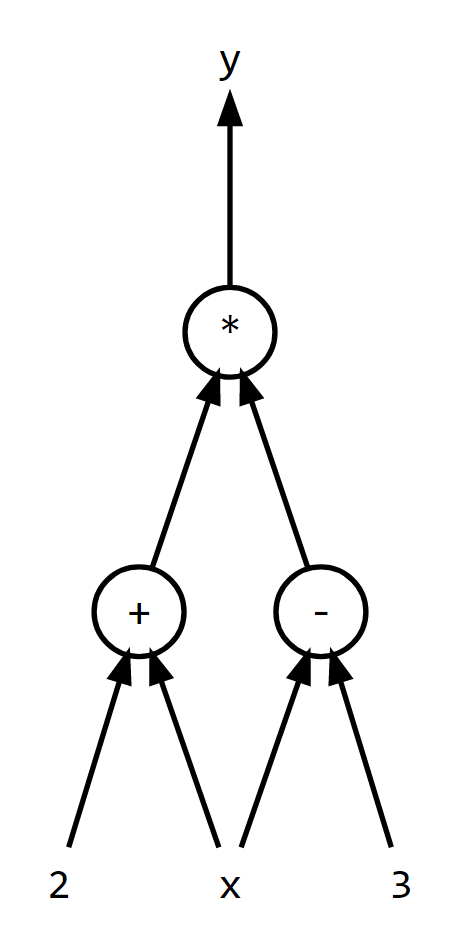
\includegraphics[width=5.5in,height=3.5in]{./intro_files/figure-latex/dot-figure-1.png}

}

\end{figure}

}

\caption{\label{fig-compTreeSimple}Ausdrucksbaum zum Ausdruck
\texttt{y\ =\ (2\ +\ x)\ *\ (x\ -\ 3)}.}

\end{figure}

Wir wollen nun unsere Python-Funktion so umschreiben, dass diese
Struktur auch im Funktionskörper sichtbar wird. Dazu führen wir drei
Hilfsvariablen \texttt{v0,\ v1,\ v2} ein.

\begin{Shaded}
\begin{Highlighting}[]
\KeywordTok{def}\NormalTok{ f(x):}
\NormalTok{    v0 }\OperatorTok{=}\NormalTok{ x}
\NormalTok{    v1 }\OperatorTok{=} \DecValTok{2} \OperatorTok{+}\NormalTok{ v0}
\NormalTok{    v2 }\OperatorTok{=}\NormalTok{ v0 }\OperatorTok{{-}} \DecValTok{3}
\NormalTok{    y }\OperatorTok{=}\NormalTok{ v1 }\OperatorTok{*}\NormalTok{ v2}
    \ControlFlowTok{return}\NormalTok{ y}
\end{Highlighting}
\end{Shaded}

\end{example}

\begin{center}\rule{0.5\linewidth}{0.5pt}\end{center}

\begin{tcolorbox}[enhanced jigsaw, title=\textcolor{quarto-callout-important-color}{\faExclamation}\hspace{0.5em}{Konvention}, colbacktitle=quarto-callout-important-color!10!white, bottomrule=.15mm, titlerule=0mm, colback=white, breakable, colframe=quarto-callout-important-color-frame, bottomtitle=1mm, toptitle=1mm, leftrule=.75mm, arc=.35mm, left=2mm, rightrule=.15mm, toprule=.15mm, opacitybacktitle=0.6, opacityback=0, coltitle=black]
Eine Funktion berechnet aus einem Argument \texttt{x} einen Rückgabewert
\texttt{y} über eine Reihe von Hilfsvariablen \texttt{v}, die mit
aufsteigenden Indizes versehen sind. Dabei setzen wir am Anfang immer
\texttt{v0\ =\ x}.
\end{tcolorbox}

\leavevmode\vadjust pre{\hypertarget{exr-ProgToFun}{}}%
\begin{exercise}[Programm in Funktion übersetzen]\label{exr-ProgToFun}

Schreibe die mathematische Funktion auf, die durch das folgende Programm
berechnet wird.

\begin{Shaded}
\begin{Highlighting}[]
\ImportTok{import}\NormalTok{ math}

\KeywordTok{def}\NormalTok{ f(x):}
\NormalTok{    v0 }\OperatorTok{=}\NormalTok{ x}
\NormalTok{    v1 }\OperatorTok{=}\NormalTok{ v0 }\OperatorTok{**} \DecValTok{2}
\NormalTok{    v2 }\OperatorTok{=}\NormalTok{ v1 }\OperatorTok{+} \DecValTok{2}
\NormalTok{    v3 }\OperatorTok{=} \OperatorTok{{-}}\NormalTok{v1 }\OperatorTok{/} \DecValTok{2}
\NormalTok{    v4 }\OperatorTok{=}\NormalTok{ math.cos(v2)}
\NormalTok{    v5 }\OperatorTok{=}\NormalTok{ math.exp(v3)}
\NormalTok{    v6 }\OperatorTok{=}\NormalTok{ v4 }\OperatorTok{*}\NormalTok{ v5}
\NormalTok{    y }\OperatorTok{=}\NormalTok{ v6 }\OperatorTok{+} \DecValTok{1} \OperatorTok{/}\NormalTok{ v0}
    \ControlFlowTok{return}\NormalTok{ y }
\end{Highlighting}
\end{Shaded}

\end{exercise}

\begin{tcolorbox}[enhanced jigsaw, title=\textcolor{quarto-callout-tip-color}{\faLightbulb}\hspace{0.5em}{Lösung}, colbacktitle=quarto-callout-tip-color!10!white, bottomrule=.15mm, titlerule=0mm, colback=white, breakable, colframe=quarto-callout-tip-color-frame, bottomtitle=1mm, toptitle=1mm, leftrule=.75mm, arc=.35mm, left=2mm, rightrule=.15mm, toprule=.15mm, opacitybacktitle=0.6, opacityback=0, coltitle=black]
\[
\begin{flalign}
v_1 & = x^2 \\
v_2 & = x^2 + 2 \\
v_3 & = - \frac{x^2}{2} \\
v_4 & = \cos(x^2 + 2) \\
v_5 & = e^{- \frac{x^2}{2}} \\
v_6 & = \cos(x^2 + 2) \cdot e^{- \frac{x^2}{2}} \\
y & = f(x) = \cos(x^2 + 2) \cdot e^{- \frac{x^2}{2}} + \frac{1}{x} \\
\end{flalign}
\]
\end{tcolorbox}

\leavevmode\vadjust pre{\hypertarget{exr-FunToGraphProg}{}}%
\begin{exercise}[Funktion in Graph und Programm
übersetzen]\label{exr-FunToGraphProg}

Schreibe zur mathematischen Funktion
\(y = f(x) = \frac{\ln(x^2 + 1)}{\sqrt{x^2 + 1 + x}}\) den Ausdrucksbaum
auf. Übersetze den Ausdruck anschliessend in eine Python-Funktion gemäss
der Konvention.

\end{exercise}

\begin{tcolorbox}[enhanced jigsaw, title=\textcolor{quarto-callout-tip-color}{\faLightbulb}\hspace{0.5em}{Lösung}, colbacktitle=quarto-callout-tip-color!10!white, bottomrule=.15mm, titlerule=0mm, colback=white, breakable, colframe=quarto-callout-tip-color-frame, bottomtitle=1mm, toptitle=1mm, leftrule=.75mm, arc=.35mm, left=2mm, rightrule=.15mm, toprule=.15mm, opacitybacktitle=0.6, opacityback=0, coltitle=black]

\begin{figure}

{\centering 

\begin{figure}[H]

{\centering 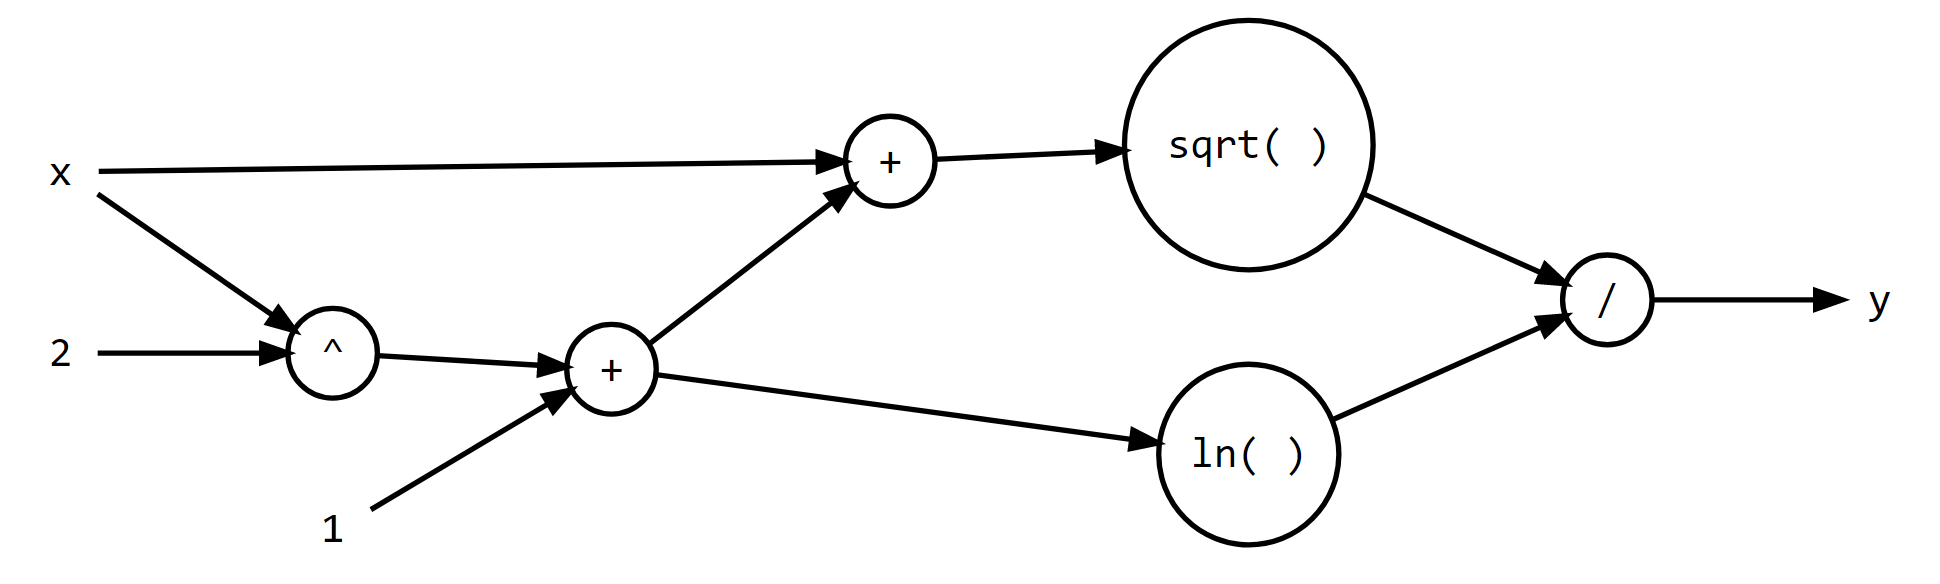
\includegraphics[width=5.5in,height=3.5in]{./intro_files/figure-latex/dot-figure-2.png}

}

\end{figure}

}

\caption{\label{fig-compTreeSimple}Computational Graph zum Ausdruck
\texttt{y\ =\ ln(x\^{}2\ +\ 1)\ /\ sqrt(x\^{}2\ +\ 1\ +\ x)}.}

\end{figure}

\begin{Shaded}
\begin{Highlighting}[]
\ImportTok{import}\NormalTok{ math}

\KeywordTok{def}\NormalTok{ f(x):}
\NormalTok{    v0 }\OperatorTok{=}\NormalTok{ x}
\NormalTok{    v1 }\OperatorTok{=}\NormalTok{ v0 }\OperatorTok{**} \DecValTok{2}
\NormalTok{    v2 }\OperatorTok{=}\NormalTok{ v1 }\OperatorTok{+} \DecValTok{1}
\NormalTok{    v3 }\OperatorTok{=}\NormalTok{ v2 }\OperatorTok{+}\NormalTok{ v0}
\NormalTok{    v4 }\OperatorTok{=}\NormalTok{ math.log(v2)}
\NormalTok{    v5 }\OperatorTok{=}\NormalTok{ math.sqrt(v3)}
\NormalTok{    y }\OperatorTok{=}\NormalTok{ v4 }\OperatorTok{/}\NormalTok{ v5}
    \ControlFlowTok{return}\NormalTok{ y}
\end{Highlighting}
\end{Shaded}

Natürlich hätte man z.B. \texttt{v3} und \texttt{v4} auch vertauschen
können.

\end{tcolorbox}

\leavevmode\vadjust pre{\hypertarget{exr-LoopProgToFun}{}}%
\begin{exercise}[Ein Programm mit einer
Schleife]\label{exr-LoopProgToFun}

Betrachte das folgende Programm:

\begin{Shaded}
\begin{Highlighting}[]
\KeywordTok{def}\NormalTok{ f(x):}
\NormalTok{    v0 }\OperatorTok{=}\NormalTok{ x}
    \ControlFlowTok{for}\NormalTok{ i }\KeywordTok{in} \BuiltInTok{range}\NormalTok{(}\DecValTok{2}\NormalTok{):}
\NormalTok{        v0 }\OperatorTok{=}\NormalTok{ v0 }\OperatorTok{**} \DecValTok{2} \OperatorTok{+} \DecValTok{1}
\NormalTok{    y }\OperatorTok{=}\NormalTok{ v0}
    \ControlFlowTok{return}\NormalTok{ y}
\end{Highlighting}
\end{Shaded}

Ersetze im Funktionskörper die Schleife durch mehrere Befehle, so dass
immer noch der gleiche mathematische Ausdruck berechnet wird und unsere
Konvention eingehalten wird. Welche mathematische Funktion wird durch
die Python-Funktion berechnet? Was ändert sich, wenn stattdessen
\texttt{for\ i\ in\ range(3)} oder \texttt{for\ i\ in\ range(4)} stehen
würde?

\end{exercise}

\begin{tcolorbox}[enhanced jigsaw, title=\textcolor{quarto-callout-tip-color}{\faLightbulb}\hspace{0.5em}{Lösung}, colbacktitle=quarto-callout-tip-color!10!white, bottomrule=.15mm, titlerule=0mm, colback=white, breakable, colframe=quarto-callout-tip-color-frame, bottomtitle=1mm, toptitle=1mm, leftrule=.75mm, arc=.35mm, left=2mm, rightrule=.15mm, toprule=.15mm, opacitybacktitle=0.6, opacityback=0, coltitle=black]

Für jeden Schleifendurchgang benötigen wir eine neue Hilfsvariable. Die
Funktion, die dabei entsteht, kann geschrieben werden als
\(f(x) = (\ell \circ \ell \circ \ldots \circ \ell)(x)\), wobei
\(\ell(x) = x^2 + 1\) ist.

\hypertarget{range2}{%
\subsubsection{\texorpdfstring{\texttt{range(2)}}{range(2)}}\label{range2}}

\begin{Shaded}
\begin{Highlighting}[]
\KeywordTok{def}\NormalTok{ f(x):}
\NormalTok{    v0 }\OperatorTok{=}\NormalTok{ x}
\NormalTok{    v1 }\OperatorTok{=}\NormalTok{ v0 }\OperatorTok{**} \DecValTok{2} \OperatorTok{+} \DecValTok{1}
\NormalTok{    v2 }\OperatorTok{=}\NormalTok{ v1 }\OperatorTok{**} \DecValTok{2} \OperatorTok{+} \DecValTok{1}
\NormalTok{    y }\OperatorTok{=}\NormalTok{ v2}
    \ControlFlowTok{return}\NormalTok{ y}
\end{Highlighting}
\end{Shaded}

\[
\begin{flalign}
    f(x) &= \ell(\ell(x)) \\ 
         &= (x^2 + 1)^2 + 1 = x^4 + 2x^2 + 2
\end{flalign}
\]

\hypertarget{range3}{%
\subsubsection{\texorpdfstring{\texttt{range(3)}}{range(3)}}\label{range3}}

\begin{Shaded}
\begin{Highlighting}[]
\KeywordTok{def}\NormalTok{ f(x):}
\NormalTok{    v0 }\OperatorTok{=}\NormalTok{ x}
\NormalTok{    v1 }\OperatorTok{=}\NormalTok{ v0 }\OperatorTok{**} \DecValTok{2} \OperatorTok{+} \DecValTok{1}
\NormalTok{    v2 }\OperatorTok{=}\NormalTok{ v1 }\OperatorTok{**} \DecValTok{2} \OperatorTok{+} \DecValTok{1}
\NormalTok{    v3 }\OperatorTok{=}\NormalTok{ v2 }\OperatorTok{**} \DecValTok{2} \OperatorTok{+} \DecValTok{1}
\NormalTok{    y }\OperatorTok{=}\NormalTok{ v3}
    \ControlFlowTok{return}\NormalTok{ y}
\end{Highlighting}
\end{Shaded}

\[
\begin{flalign}
    f(x) &= \ell(\ell(\ell(x))) \\
         &= ((x^2 + 1)^2 + 1)^2 + 1 = x^8 + 4x^6 + 8x^4 + 8x^2 + 5
\end{flalign}
\]

\hypertarget{range4}{%
\subsubsection{\texorpdfstring{\texttt{range(4)}}{range(4)}}\label{range4}}

\begin{Shaded}
\begin{Highlighting}[]
\KeywordTok{def}\NormalTok{ f(x):}
\NormalTok{    v0 }\OperatorTok{=}\NormalTok{ x}
\NormalTok{    v1 }\OperatorTok{=}\NormalTok{ v0 }\OperatorTok{**} \DecValTok{2} \OperatorTok{+} \DecValTok{1}
\NormalTok{    v2 }\OperatorTok{=}\NormalTok{ v1 }\OperatorTok{**} \DecValTok{2} \OperatorTok{+} \DecValTok{1}
\NormalTok{    v3 }\OperatorTok{=}\NormalTok{ v2 }\OperatorTok{**} \DecValTok{2} \OperatorTok{+} \DecValTok{1}
\NormalTok{    v4 }\OperatorTok{=}\NormalTok{ v3 }\OperatorTok{**} \DecValTok{2} \OperatorTok{+} \DecValTok{1}
\NormalTok{    y }\OperatorTok{=}\NormalTok{ v4}
    \ControlFlowTok{return}\NormalTok{ y}
\end{Highlighting}
\end{Shaded}

\[
\begin{flalign}
    f(x) &= \ell(\ell(\ell(\ell(x)))) \\
         &= (((x^2 + 1)^2 + 1)^2 + 1)^2 + 1 \\
         &= x^{16} + 8x^{14} + 32x^{12} + 80x^{10} + 138x^8 + 168x^6 + 144x^4 + 80x^2 + 26
\end{flalign}
\]

\end{tcolorbox}

\hypertarget{unser-ziel-programme-ableiten}{%
\section{Unser Ziel: Programme
ableiten}\label{unser-ziel-programme-ableiten}}

Wie eingangs erwähnt wurde, haben Ableitungen viele nützliche
Anwendungen.

Wir möchten nun Ableitungen von Funktionen berechnen, die durch
Programme beschrieben werden, die wie oben einen numerischen Parameter
\texttt{x} als Input erhalten und einen numerischen Wert \texttt{y}
zurückliefern. Unser Ziel wird es sein, die Programme so zu
modifizieren, dass der Funktionsaufruf \texttt{f(x0)} nicht nur den
Funktionswert \(f(x_0)\) zurückgibt, sondern auch den Wert der Ableitung
\(f'(x_0)\). Wir sind dabei nicht an einer symbolischen Ableitung
interessiert, wie das z.B. GeoGebra oder Mathematica machen (s.
Kapitel~\ref{sec-ADnotSymbDiff}), sondern nur an einer punktweisen
Auswertung. Natürlich wollen wir die Ableitungsfunktion auch nicht von
Hand bestimmen. Wir wollen uns aber auch nicht bloss mit einer
Annhäerung des Wertes der Ableitung zufrieden geben (s.
Kapitel~\ref{sec-ADnotNumDiff}), sondern den Wert von \(f'(x_0)\) bis
auf Maschinengenauigkeit exakt berechnen. In
Kapitel~\ref{sec-SADforOneDimFunctions} werden wir eine Methode kennen
lernen, die all dies leistet und dabei die Laufzeit eines Programms
nicht wesentlich erhöht. Der Name dieser Methode: Algorithmische
Differentiation (AD), obwohl die Namensgebung hier nicht eindeutig ist:

\begin{quote}
One of the obstacles in this area {[}of computing derivatives{]}, which
involves ``symbolic'' and ``numerical'' methods, has been a confusion in
terminology {[}\ldots{]}. There is not even general agreement on the
best name for the field, which is frequently referred to as
\emph{automatic} or \emph{computational differentiation} in the
literature. For this book the adjective \emph{algorithmic} seemed
preferable, because much of the material emphasizes algorithmic
structure, sometimes glossing over the details and pitfalls of actual
implementations. (Aus dem Vorwort zu Griewank und Walther (2008))
\end{quote}

Bevor wir uns aber der Methode der algorithmischen Differentiation
zuwenden, wollen wir sie durch einige Beispiele motivieren, bei denen
die Berechnung von Ableitung von Funktionen und Programmen eine zentrale
Rolle spielt: Das Newtonverfahren und das Gradient Descent Verfahren.

\hypertarget{sec-Newtonverfahren1D}{%
\subsection{Das Newtonverfahren zur Berechnung von
Nullstellen}\label{sec-Newtonverfahren1D}}

In vielen Anwendungen steht man vor der Aufgabe, die Gleichung
\(f(x) = 0\) nach \(x\) aufzulösen, d.h. eine Nullstelle \(\bar{x}\) der
Funktion zu finden. Oft ist es aber nicht möglich, die Lösung einer
solchen Gleichung in geschlossener Form darzustellen. Um dennoch eine
Lösung zumindest näherungsweise berechnen zu können, kann man
folgendermassen vorgehen:

\begin{enumerate}
\def\labelenumi{\arabic{enumi}.}
\tightlist
\item
  Wähle einen Startwert \(x_0\), der in der Nähe einer Nullstelle
  \(\bar{x}\) von \(f\) liegt.
\item
  Im Kurvenpunkt \((x_0 | y_0)\) wird die Tangente an die Kurve \(f\)
  gelegt. Deren Schnittpunkt \(x_1\) mit der \(x\)-Achse liegt in der
  Regel näher bei \(\bar{x}\) als \(x_0\).
\item
  Nun wiederholt man das Verfahren, indem man bei \(x_1\) die Tangente
  an die Kurve legt, usw. Auf diese Weise erhält man eine Folge von
  Näherungen \(x_0, x_1, x_2, \ldots\), deren Grenzwert die Nullstelle
  \(\bar{x}\) ist.
\end{enumerate}

Dieser Algorithmus ist als Newtonverfahren bekannt.

Die Gleichung der Tangente im Punkt \((x_n | y_n) = (x_n | f(x_n))\) ist
bekanntlich \(t(x) = f(x_n) + f'(x_n) \cdot (x - x_n)\). Die Nullstelle
der Tangente ist der Näherungswert \(x_{n+1}\). Aus \(t(x_{n+1}) = 0\)
ergibt sich nun die Iterationsvorschrift des Newtonverfahrens:
\begin{equation}\protect\hypertarget{eq-newton}{}{
x_{n+1} = x_n - \frac{f(x_n)}{f'(x_n)}
}\label{eq-newton}\end{equation}

\leavevmode\vadjust pre{\hypertarget{exr-NewtonFirstTry}{}}%
\begin{exercise}[Das Newtonverfahren
programmieren]\label{exr-NewtonFirstTry}

Schreibe ein Programm, das mit Hilfe des Newtonverfahrens
(Gleichung~\ref{eq-newton}) eine Nullstelle der Funktion
\(f(x) = \frac{1}{31} x^3 -\frac{1}{20} x^2 -x + 1\) berechnet. Verwende
den Startwert \(x_0 = -2\). Du kannst abbrechen, wenn die Differenz
\(|x_{n+1} - x_n|\) kleiner als eine bestimmte Toleranz wird, z.B.
kleiner als \texttt{tol\ =\ 1e-6}. Wie flexibel ist dein Programm
einsetzbar? Überlege dir z.B., wie viele Änderungen du vornehmen
müsstest, wenn du die Nullstelle einer anderen Funktion berechnen
müsstest.

\end{exercise}

\begin{tcolorbox}[enhanced jigsaw, title=\textcolor{quarto-callout-tip-color}{\faLightbulb}\hspace{0.5em}{Lösung}, colbacktitle=quarto-callout-tip-color!10!white, bottomrule=.15mm, titlerule=0mm, colback=white, breakable, colframe=quarto-callout-tip-color-frame, bottomtitle=1mm, toptitle=1mm, leftrule=.75mm, arc=.35mm, left=2mm, rightrule=.15mm, toprule=.15mm, opacitybacktitle=0.6, opacityback=0, coltitle=black]

Welche der folgenden Lösungsvorschläge kommt deinem Programm am
nächsten?

\hypertarget{version-1}{%
\subsubsection{Version 1}\label{version-1}}

\begin{Shaded}
\begin{Highlighting}[]
\ImportTok{from}\NormalTok{ math }\ImportTok{import}\NormalTok{ fabs}

\NormalTok{x0 }\OperatorTok{=} \OperatorTok{{-}}\DecValTok{2}
\NormalTok{tol }\OperatorTok{=} \FloatTok{1e{-}6}
\CommentTok{\# Erster Schritt berechnen}
\NormalTok{x1 }\OperatorTok{=}\NormalTok{ x0 }\OperatorTok{{-}}\NormalTok{ (}\DecValTok{1}\OperatorTok{/}\DecValTok{31} \OperatorTok{*}\NormalTok{ x0}\OperatorTok{**}\DecValTok{3} \OperatorTok{{-}} \DecValTok{1}\OperatorTok{/}\DecValTok{20} \OperatorTok{*}\NormalTok{ x0}\OperatorTok{**}\DecValTok{2} \OperatorTok{{-}}\NormalTok{ x0 }\OperatorTok{+} \DecValTok{1}\NormalTok{) }\OperatorTok{/}\NormalTok{ (}\DecValTok{3}\OperatorTok{/}\DecValTok{31} \OperatorTok{*}\NormalTok{ x0}\OperatorTok{**}\DecValTok{2} \OperatorTok{{-}} \DecValTok{1}\OperatorTok{/}\DecValTok{10} \OperatorTok{*}\NormalTok{ x0 }\OperatorTok{{-}} \DecValTok{1}\NormalTok{)}
\ControlFlowTok{while}\NormalTok{ fabs(x1 }\OperatorTok{{-}}\NormalTok{ x0) }\OperatorTok{\textgreater{}}\NormalTok{ tol:}
\NormalTok{    x0 }\OperatorTok{=}\NormalTok{ x1}
\NormalTok{    x1 }\OperatorTok{=}\NormalTok{ x0 }\OperatorTok{{-}}\NormalTok{ (}\DecValTok{1}\OperatorTok{/}\DecValTok{31} \OperatorTok{*}\NormalTok{ x0}\OperatorTok{**}\DecValTok{3} \OperatorTok{{-}} \DecValTok{1}\OperatorTok{/}\DecValTok{20} \OperatorTok{*}\NormalTok{ x0}\OperatorTok{**}\DecValTok{2} \OperatorTok{{-}}\NormalTok{ x0 }\OperatorTok{+} \DecValTok{1}\NormalTok{) }\OperatorTok{/}\NormalTok{ (}\DecValTok{3}\OperatorTok{/}\DecValTok{31} \OperatorTok{*}\NormalTok{ x0}\OperatorTok{**}\DecValTok{2} \OperatorTok{{-}} \DecValTok{1}\OperatorTok{/}\DecValTok{10} \OperatorTok{*}\NormalTok{ x0 }\OperatorTok{{-}} \DecValTok{1}\NormalTok{)}
\BuiltInTok{print}\NormalTok{(x1)}
\end{Highlighting}
\end{Shaded}

\begin{verbatim}
5.908619865450271
\end{verbatim}

Das Newtonverfahren wird als main-Funktion (d.h. im Hauptprogramm)
ausgeführt. Braucht man jedoch die Nullstelle einer anderen Funktion,
dann muss ein neues Programm geschrieben werden. Die Ableitung wurde von
Hand berechnet.

\hypertarget{version-2}{%
\subsubsection{Version 2}\label{version-2}}

\begin{Shaded}
\begin{Highlighting}[]
\ImportTok{from}\NormalTok{ math }\ImportTok{import}\NormalTok{ fabs}

\KeywordTok{def}\NormalTok{ f(x):}
\NormalTok{    y }\OperatorTok{=} \DecValTok{1}\OperatorTok{/}\DecValTok{31} \OperatorTok{*}\NormalTok{ x}\OperatorTok{**}\DecValTok{3} \OperatorTok{{-}} \DecValTok{1}\OperatorTok{/}\DecValTok{20} \OperatorTok{*}\NormalTok{ x}\OperatorTok{**}\DecValTok{2} \OperatorTok{{-}}\NormalTok{ x }\OperatorTok{+} \DecValTok{1}
    \ControlFlowTok{return}\NormalTok{ y}

\KeywordTok{def}\NormalTok{ fdot(x):}
\NormalTok{    ydot }\OperatorTok{=} \DecValTok{3}\OperatorTok{/}\DecValTok{31} \OperatorTok{*}\NormalTok{ x}\OperatorTok{**}\DecValTok{2} \OperatorTok{{-}} \DecValTok{1}\OperatorTok{/}\DecValTok{10} \OperatorTok{*}\NormalTok{ x }\OperatorTok{{-}} \DecValTok{1}
    \ControlFlowTok{return}\NormalTok{ ydot}

\NormalTok{x0 }\OperatorTok{=} \OperatorTok{{-}}\DecValTok{2}
\NormalTok{tol }\OperatorTok{=} \FloatTok{1e{-}6}
\CommentTok{\# Erster Schritt berechnen}
\NormalTok{x1 }\OperatorTok{=}\NormalTok{ x0 }\OperatorTok{{-}}\NormalTok{ f(x0) }\OperatorTok{/}\NormalTok{ fdot(x0)}
\ControlFlowTok{while}\NormalTok{ fabs(x1 }\OperatorTok{{-}}\NormalTok{ x0) }\OperatorTok{\textgreater{}}\NormalTok{ tol:}
\NormalTok{    x0 }\OperatorTok{=}\NormalTok{ x1}
\NormalTok{    x1 }\OperatorTok{=}\NormalTok{ x0 }\OperatorTok{{-}}\NormalTok{ f(x0) }\OperatorTok{/}\NormalTok{ fdot(x0)}
\BuiltInTok{print}\NormalTok{(x1)}
\end{Highlighting}
\end{Shaded}

\begin{verbatim}
5.908619865450271
\end{verbatim}

Das Newtonverfahren wird als main-Funktion (d.h. im Hauptprogramm)
ausgeführt, aber die Berechnung von \(f\) und ihrer Ableitung \(f'\)
wurde in zwei Funktionen \texttt{f} und \texttt{fdot} ausgelagert. Das
macht das Programm übersichtlicher und flexibler. Die Ableitung wurde
wieder von Hand berechnet.

\hypertarget{version-3}{%
\subsubsection{Version 3}\label{version-3}}

\begin{Shaded}
\begin{Highlighting}[]
\ImportTok{from}\NormalTok{ math }\ImportTok{import}\NormalTok{ fabs}

\KeywordTok{def}\NormalTok{ newton(f, fdot, x0):}
\NormalTok{    tol }\OperatorTok{=} \FloatTok{1e{-}6}
    \CommentTok{\# Erster Schritt berechnen}
\NormalTok{    x1 }\OperatorTok{=}\NormalTok{ x0 }\OperatorTok{{-}}\NormalTok{ f(x0) }\OperatorTok{/}\NormalTok{ fdot(x0)}
    \ControlFlowTok{while}\NormalTok{ fabs(x1 }\OperatorTok{{-}}\NormalTok{ x0) }\OperatorTok{\textgreater{}}\NormalTok{ tol:}
\NormalTok{        x0 }\OperatorTok{=}\NormalTok{ x1}
\NormalTok{        x1 }\OperatorTok{=}\NormalTok{ x0 }\OperatorTok{{-}}\NormalTok{ f(x0) }\OperatorTok{/}\NormalTok{ fdot(x0)}
    \ControlFlowTok{return}\NormalTok{ x1}

\KeywordTok{def}\NormalTok{ f(x):}
\NormalTok{    y }\OperatorTok{=} \DecValTok{1}\OperatorTok{/}\DecValTok{31} \OperatorTok{*}\NormalTok{ x}\OperatorTok{**}\DecValTok{3} \OperatorTok{{-}} \DecValTok{1}\OperatorTok{/}\DecValTok{20} \OperatorTok{*}\NormalTok{ x}\OperatorTok{**}\DecValTok{2} \OperatorTok{{-}}\NormalTok{ x }\OperatorTok{+} \DecValTok{1}
    \ControlFlowTok{return}\NormalTok{ y}

\KeywordTok{def}\NormalTok{ fdot(x):}
\NormalTok{    ydot }\OperatorTok{=} \DecValTok{3}\OperatorTok{/}\DecValTok{31} \OperatorTok{*}\NormalTok{ x}\OperatorTok{**}\DecValTok{2} \OperatorTok{{-}} \DecValTok{1}\OperatorTok{/}\DecValTok{10} \OperatorTok{*}\NormalTok{ x }\OperatorTok{{-}} \DecValTok{1}
    \ControlFlowTok{return}\NormalTok{ ydot}

\NormalTok{x0 }\OperatorTok{=} \OperatorTok{{-}}\DecValTok{2}
\NormalTok{xbar }\OperatorTok{=}\NormalTok{ newton(f, fdot, x0)}
\BuiltInTok{print}\NormalTok{(xbar)}
\end{Highlighting}
\end{Shaded}

\begin{verbatim}
5.908619865450271
\end{verbatim}

Das Newtonverfahren wird als eigene Funktion
\texttt{newton(f,\ fdot,\ x0)} implementiert. Dieser werden die Funktion
\(f\) und ihre Ableitung \(f'\), sowie der Startwert \(x_0\) als
Argumente übergeben. Sie kann dann im Hauptprogramm aufgerufen werden.
Die Ableitung wurde aber immer noch von Hand berechnet.

\hypertarget{version-4}{%
\subsubsection{Version 4}\label{version-4}}

\begin{Shaded}
\begin{Highlighting}[]
\ImportTok{from}\NormalTok{ math }\ImportTok{import}\NormalTok{ fabs}

\KeywordTok{def}\NormalTok{ newton(f, x0):}
\NormalTok{    tol }\OperatorTok{=} \FloatTok{1e{-}6}
    \CommentTok{\# Erster Schritt berechnen}
    \CommentTok{\# Ableitung von f an der Stelle x0 annähern}
\NormalTok{    h }\OperatorTok{=} \FloatTok{1e{-}6}
\NormalTok{    ydot }\OperatorTok{=}\NormalTok{ ( f(x0 }\OperatorTok{+}\NormalTok{ h) }\OperatorTok{{-}}\NormalTok{ f(x0) ) }\OperatorTok{/}\NormalTok{ h}
\NormalTok{    x1 }\OperatorTok{=}\NormalTok{ x0 }\OperatorTok{{-}}\NormalTok{ f(x0) }\OperatorTok{/}\NormalTok{ ydot}
    \ControlFlowTok{while}\NormalTok{ fabs(x1 }\OperatorTok{{-}}\NormalTok{ x0) }\OperatorTok{\textgreater{}}\NormalTok{ tol:}
\NormalTok{        x0 }\OperatorTok{=}\NormalTok{ x1}
\NormalTok{        ydot }\OperatorTok{=}\NormalTok{ ( f(x0 }\OperatorTok{+}\NormalTok{ h) }\OperatorTok{{-}}\NormalTok{ f(x0) ) }\OperatorTok{/}\NormalTok{ h}
\NormalTok{        x1 }\OperatorTok{=}\NormalTok{ x0 }\OperatorTok{{-}}\NormalTok{ f(x0) }\OperatorTok{/}\NormalTok{ ydot}
    \ControlFlowTok{return}\NormalTok{ x1}

\KeywordTok{def}\NormalTok{ f(x):}
\NormalTok{    y }\OperatorTok{=} \DecValTok{1}\OperatorTok{/}\DecValTok{31} \OperatorTok{*}\NormalTok{ x}\OperatorTok{**}\DecValTok{3} \OperatorTok{{-}} \DecValTok{1}\OperatorTok{/}\DecValTok{20} \OperatorTok{*}\NormalTok{ x}\OperatorTok{**}\DecValTok{2} \OperatorTok{{-}}\NormalTok{ x }\OperatorTok{+} \DecValTok{1}
    \ControlFlowTok{return}\NormalTok{ y}

\NormalTok{x0 }\OperatorTok{=} \OperatorTok{{-}}\DecValTok{2}
\NormalTok{xbar }\OperatorTok{=}\NormalTok{ newton(f, x0)}
\BuiltInTok{print}\NormalTok{(xbar)}
\end{Highlighting}
\end{Shaded}

\begin{verbatim}
5.90861986545027
\end{verbatim}

Hier wird das Newtonverfahren in einer Funktion implementiert. Die
Ableitung wird nicht mehr von Hand berechnet, sondern innerhalb der
Funktion mit \(f'(x_0)\approx \frac{f(x_0 + h) - f(x_0)}{h}\)
angenähert. Dabei wird einfach \texttt{h\ =\ 1e-6} gesetzt und gehofft,
dass der entstehende Rundungsfehler klein genug ist. Beachte aber, dass
sich der berechnete Wert von der Ausgabe in den anderen Versionen leicht
unterscheidet.

\end{tcolorbox}

Auch die Version 4 der vorgestellten Lösung ist noch nicht befriedigend.
Als wir die Ableitung von Hand berechnet hatten, musste nur die Funktion
\texttt{fdot} and der Stelle \texttt{x0} ausgewertet werden, um den (bis
auf Maschinengenauigkeit) \emph{exakten} Wert von \(f'(x_0)\) zu
erhalten. Bei der letzten Methode muss man sich mit einem Näherungswert
der Ableitung zufrieden geben. Auch wenn der Wert in diesem Beispiel gut
genug war\footnote{Dieser Ansatz kann verbessert werden indem man z.B.
  \(f'(x_0) \approx \frac{f(x_0 + h) - f(x_0 - h)}{2h}\) verwendet. Die
  im Beispiel beschriebenen Probleme bleiben aber auch dann bestehen.},
so haben wir doch keine Garantie, dass wir für alle Funktionen einen
vernünftigen Wert erhalten. Auf die Probleme, die mit dieser Annäherung
von \(f'(x_0)\) auftreten, wird in Kapitel~\ref{sec-ADnotNumDiff} näher
eingegangen.

\leavevmode\vadjust pre{\hypertarget{exm-Billard}{}}%
\begin{example}[Billard auf einem runden Tisch]\label{exm-Billard}

Wir betrachten ein Beispiel aus Gander (2015). Platziere die weisse und
die blaue Billardkugel auf dem runden Tisch. Das Ziel ist es, die weisse
Kugel so anzustossen, dass sie die blaue Kugel trifft, nachdem sie
vorher genau einmal an die Bande gespielt wurde.

Aus Symmetriegründen dürfen wir annehmen, dass der Rand des
Billardtisches der Einheitskreis ist und dass die weisse Kugel auf der
\(x\)-Achse liegt. Die blaue Kugel habe die Koordinaten \((x_P|y_P)\).
Weiter sei \(X\) der Punkt auf dem Einheitskreis, an dem die weisse
Kugel abprallt. Wir beschreiben diesen Punkt mit seinen Polarkoordinaten
\(X=(\cos(x)|\sin(x))\). Unser Ziel ist es, \(x\) so zu berechnen, dass
die weisse Kugel die blaue trifft, nachdem sie bei \(X\) an die Bande
gestossen ist. Dabei verhält sie sich so, als ob sie an der
Kreistangente in \(X\) reflektiert wird. Der Tangentenvektor im Punkt
\(X\) lautet
\(\vec{t} = \begin{pmatrix} -\sin(x) \\ \cos(x) \end{pmatrix}\).

\begin{marginfigure}

{\centering 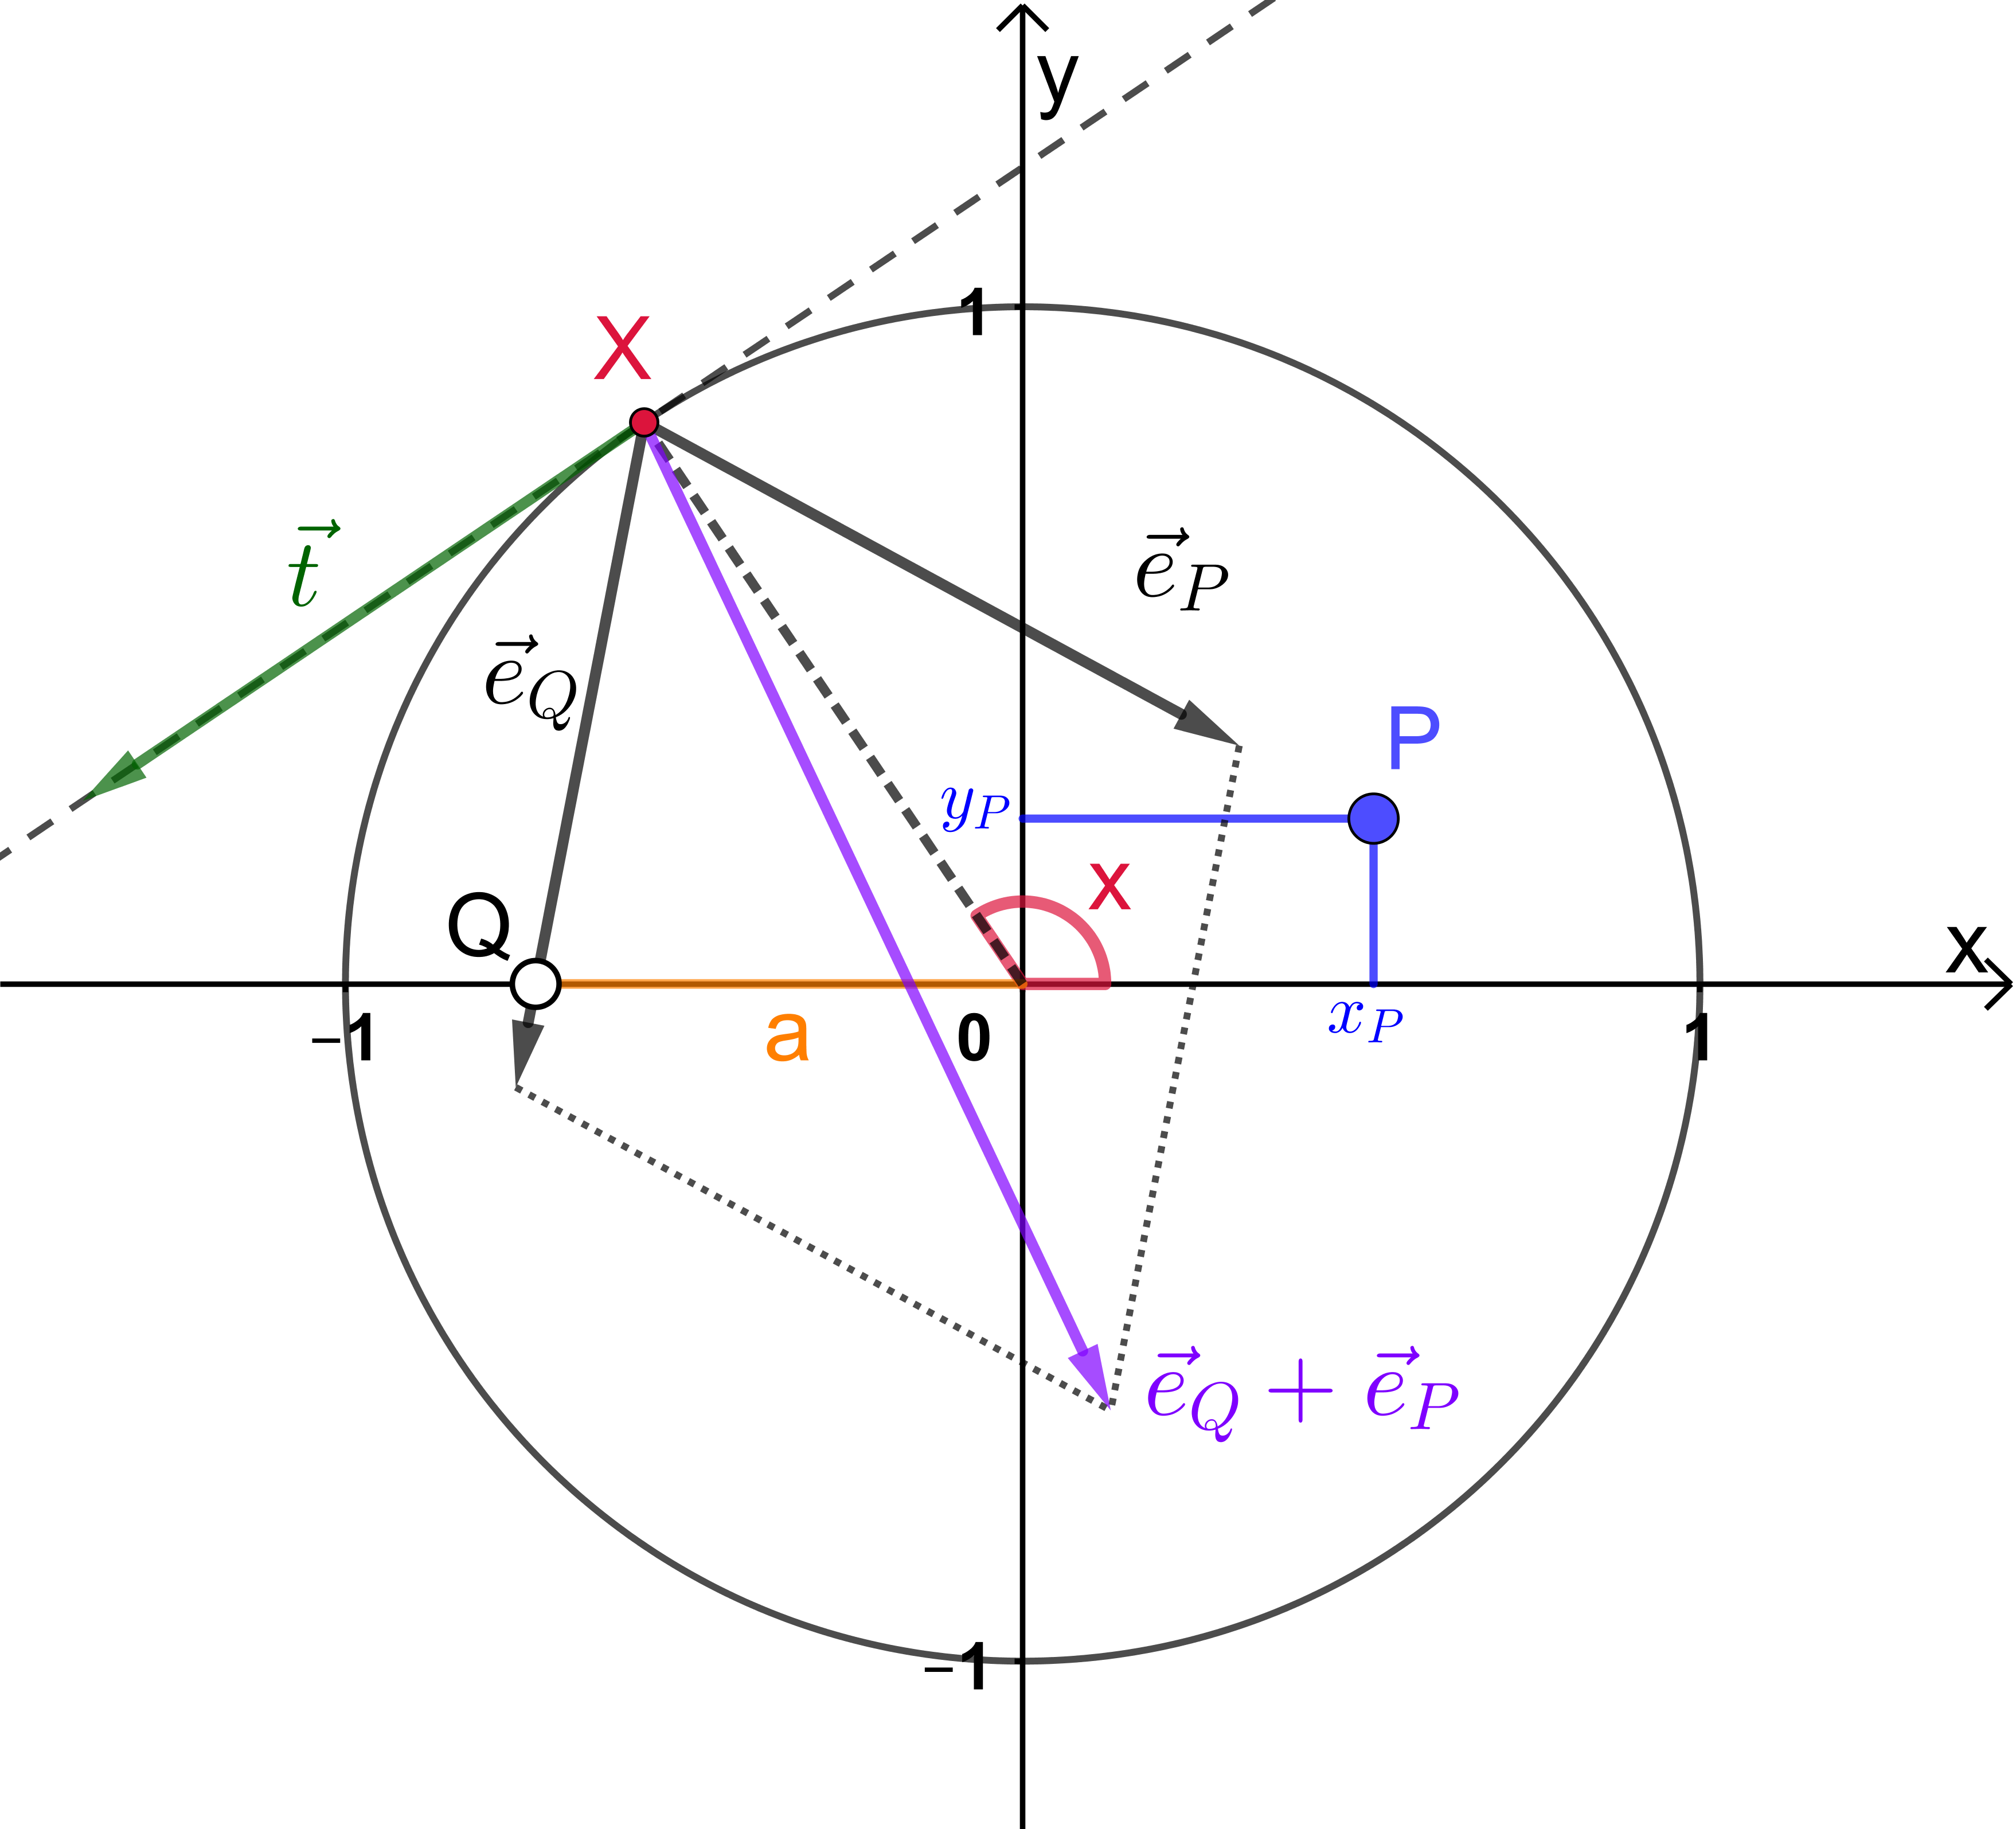
\includegraphics{./CircularBillard_sketch.png}

}

\caption{Billard auf einem runden Tisch}

\end{marginfigure}

Wir betrachten nun die Einheitsvektoren \(\vec{e}_Q\) in Richtung
\(\overrightarrow{XQ}\) und \(\vec{e}_P\) in Richtung
\(\overrightarrow{XP}\). Wenn die weisse Kugel die blaue treffen soll,
dann müssen die Winkel zwischen der Tangente und diesen Vektoren gleich
sein. Das ist genau dann der Fall, wenn \(\vec{t}\) senkrecht steht auf
\(\vec{e}_Q + \vec{e}_P\). Wir müssen also \(x\) so bestimmen, dass
\(\vec{t} \cdot (\vec{e}_Q + \vec{e}_P) = 0\) ist.

Das folgende Programm berechnet das Skalarprodukt der linken Seite
dieser Gleichung.

\begin{Shaded}
\begin{Highlighting}[]
\ImportTok{import}\NormalTok{ math}
\ImportTok{import}\NormalTok{ matplotlib.pyplot }\ImportTok{as}\NormalTok{ plt}

\KeywordTok{def}\NormalTok{ f(x):}
    \CommentTok{\# Parameter}
\NormalTok{    a }\OperatorTok{=} \OperatorTok{{-}}\FloatTok{0.8}           \CommentTok{\# Position von Q = (a|0)}
\NormalTok{    px, py }\OperatorTok{=} \FloatTok{0.5}\NormalTok{, }\FloatTok{0.5}  \CommentTok{\# Position von P = (px|py)}

    \CommentTok{\# Berechnung des Skalarprodukts}
\NormalTok{    v0 }\OperatorTok{=}\NormalTok{ x}
\NormalTok{    v1 }\OperatorTok{=}\NormalTok{ math.cos(v0)  }\CommentTok{\# x{-}Koordinate von X}
\NormalTok{    v2 }\OperatorTok{=}\NormalTok{ math.sin(v0)  }\CommentTok{\# y{-}Koordinate von X}
\NormalTok{    v3 }\OperatorTok{=}\NormalTok{ px }\OperatorTok{{-}}\NormalTok{ v1       }\CommentTok{\# x{-}Komponente des Vektors XP}
\NormalTok{    v4 }\OperatorTok{=}\NormalTok{ py }\OperatorTok{{-}}\NormalTok{ v2       }\CommentTok{\# y{-}Komponente des Vektors XP}
\NormalTok{    v5 }\OperatorTok{=}\NormalTok{ math.sqrt(v3}\OperatorTok{**}\DecValTok{2} \OperatorTok{+}\NormalTok{ v4}\OperatorTok{**}\DecValTok{2}\NormalTok{)  }\CommentTok{\# Länge des Vektors XP}
\NormalTok{    v6 }\OperatorTok{=}\NormalTok{ v3 }\OperatorTok{/}\NormalTok{ v5       }\CommentTok{\# x{-}Komponente des Einheitsvektors eP}
\NormalTok{    v7 }\OperatorTok{=}\NormalTok{ v4 }\OperatorTok{/}\NormalTok{ v5       }\CommentTok{\# y{-}Komponente des Einheitsvektors eP}
    
\NormalTok{    v8 }\OperatorTok{=}\NormalTok{ a }\OperatorTok{{-}}\NormalTok{ v1        }\CommentTok{\# x{-}Komponente des Vektors XQ}
\NormalTok{    v9 }\OperatorTok{=} \OperatorTok{{-}}\NormalTok{v2           }\CommentTok{\# y{-}Komponente des Vektors XQ}
\NormalTok{    v10 }\OperatorTok{=}\NormalTok{ math.sqrt(v8}\OperatorTok{**}\DecValTok{2} \OperatorTok{+}\NormalTok{ v9}\OperatorTok{**}\DecValTok{2}\NormalTok{)  }\CommentTok{\# Länge des Vektors XQ}
\NormalTok{    v11 }\OperatorTok{=}\NormalTok{ v8 }\OperatorTok{/}\NormalTok{ v10     }\CommentTok{\# x{-}Komponente des Vektors eQ    }
\NormalTok{    v12 }\OperatorTok{=}\NormalTok{ v9 }\OperatorTok{/}\NormalTok{ v10     }\CommentTok{\# y{-}Komponente des Vektors eQ   }
\NormalTok{    y }\OperatorTok{=}\NormalTok{ (v6 }\OperatorTok{+}\NormalTok{ v11) }\OperatorTok{*}\NormalTok{ v2 }\OperatorTok{{-}}\NormalTok{ (v7 }\OperatorTok{+}\NormalTok{ v12) }\OperatorTok{*}\NormalTok{ v1  }\CommentTok{\# Skalarprodukt}
    \ControlFlowTok{return}\NormalTok{ y   }

\CommentTok{\# Graph der Funktion f(x) plotten}
\NormalTok{fig }\OperatorTok{=}\NormalTok{ plt.figure()}
\NormalTok{ax }\OperatorTok{=}\NormalTok{ plt.gca()}
\NormalTok{ax.set\_xlim((}\DecValTok{0}\NormalTok{,}\DecValTok{2}\OperatorTok{*}\NormalTok{math.pi))}
\NormalTok{ax.set\_ylim((}\OperatorTok{{-}}\FloatTok{1.5}\NormalTok{,}\FloatTok{1.5}\NormalTok{))}
\NormalTok{X }\OperatorTok{=}\NormalTok{ [}\DecValTok{2}\OperatorTok{*}\NormalTok{math.pi }\OperatorTok{*}\NormalTok{ k }\OperatorTok{/} \DecValTok{1000} \ControlFlowTok{for}\NormalTok{ k }\KeywordTok{in} \BuiltInTok{range}\NormalTok{(}\DecValTok{1001}\NormalTok{)]}
\NormalTok{Y }\OperatorTok{=}\NormalTok{ [f(x) }\ControlFlowTok{for}\NormalTok{ x }\KeywordTok{in}\NormalTok{ X]}
\NormalTok{plt.plot([}\DecValTok{0}\NormalTok{, }\DecValTok{2}\OperatorTok{*}\NormalTok{math.pi], [}\DecValTok{0}\NormalTok{, }\DecValTok{0}\NormalTok{], }\StringTok{\textquotesingle{}k{-}{-}\textquotesingle{}}\NormalTok{) }\CommentTok{\# x{-}Achse}
\NormalTok{plt.plot(X,Y)}
\NormalTok{plt.xticks([}\DecValTok{0}\NormalTok{, math.pi}\OperatorTok{/}\DecValTok{2}\NormalTok{, math.pi, }\DecValTok{3}\OperatorTok{*}\NormalTok{math.pi}\OperatorTok{/}\DecValTok{2}\NormalTok{, }\DecValTok{2}\OperatorTok{*}\NormalTok{math.pi],}
\NormalTok{           [}\StringTok{\textquotesingle{}0\textquotesingle{}}\NormalTok{, }\StringTok{\textquotesingle{}π/2\textquotesingle{}}\NormalTok{, }\StringTok{\textquotesingle{}π\textquotesingle{}}\NormalTok{, }\StringTok{\textquotesingle{}3π/2\textquotesingle{}}\NormalTok{, }\StringTok{\textquotesingle{}2π\textquotesingle{}}\NormalTok{])}
\NormalTok{plt.show()  }
\end{Highlighting}
\end{Shaded}

\begin{figure}[H]

{\centering 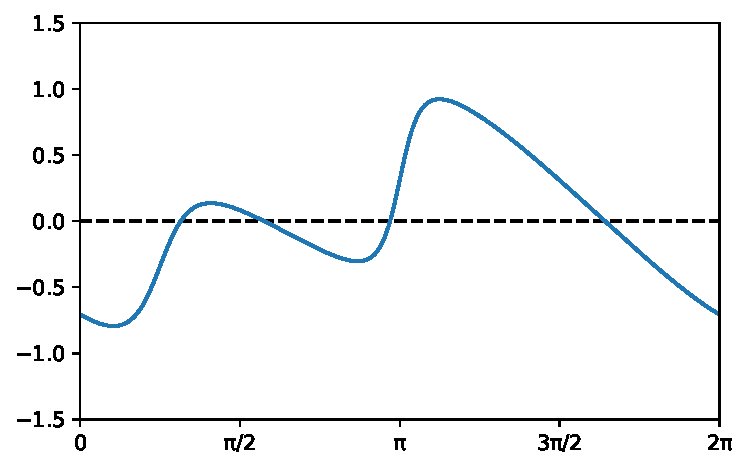
\includegraphics{./intro_files/figure-pdf/fig-graphofbillard-output-1.pdf}

}

\caption{\label{fig-graphofbillard}Graph des Skalarprodukts als Funktion
des Polarwinkels \(x\) des Punktes \(X = (cos(x) | sin(x))\). Die
Nullstellen entsprechen den Winkeln, bei denen die weisse Kugel die
blaue Kugel trifft, nachdem sie genau einmal an die Bande gespielt
wurde.}

\end{figure}

Wir möchten die Nullstellen der Funktion \texttt{f(x)} mit unserer
Funtion \texttt{newton} bestimmmen. Dazu müssen wir jedoch die Ableitung
von \texttt{f} berechnen.

\end{example}

\begin{center}\rule{0.5\linewidth}{0.5pt}\end{center}

\hypertarget{gradient-descent-zum-auffinden-lokaler-minima}{%
\subsection{Gradient Descent zum Auffinden lokaler
Minima}\label{gradient-descent-zum-auffinden-lokaler-minima}}

Eine weitere wichtige Aufgabe besteht darin, ein Minimum einer Funktion
zu finden. Auch hier wollen wir mit Hilfe der Ableitung eine Folge von
Näherungswerten \(x_0, x_1, x_2, \ldots\) finden, deren Grenzwert die
\(x\)-Koordinate eines (lokalen) Minimums von \(f\) ist.

Wenn \(f'(x_n)>0\) ist, dann wissen wir, dass die Funktion \(f\) an der
Stelle \(x_0\) streng monoton wachsend ist. D.h., dass die
Funktionswerte links von \(x_n\) kleiner sind, als an der Stelle
\(x_n\). Analog gilt, dass wenn \(f'(x_n)<0\) ist, die Funktion monoton
fallend ist und wir uns nach rechts bewegen sollten, um ein Minimum zu
finden. In der Nähe eines Minimums ist ausserdem \(|f'(x)|\) sehr klein
und wir können entsprechend kleinere Schritte machen, um uns diesem
anzunähern. Um also von \(x_n\) zu \(x_{n+1}\) zu kommen, machen wir
einen Schritt, der proportional zu \(-f'(x_n)\) ist. Mit dem
Proporionalitätsfaktor \(\lambda\in\mathbb{R}\) und einem geeignet
gewählten Startwert \(x_0\) erhalten wir die Iterationsvorschrift
\begin{equation}\protect\hypertarget{eq-gradientDescent}{}{
x_{n+1} = x_n - \lambda\cdot f'(x_n)
}\label{eq-gradientDescent}\end{equation}

\leavevmode\vadjust pre{\hypertarget{exr-GradientDescentBasicProperties}{}}%
\begin{exercise}[Eigenschaften der Gradient Descent
Methode]\label{exr-GradientDescentBasicProperties}

Experimentiere mit verschiedenen Funktionen und verschiedenen
Schrittweiten \(\lambda\). Was passiert, wenn die Schrittweite zu klein
bzw. zu gross gewählt wird? Was passiert, wenn \(f\) an der Stelle
\(x_0\) ein lokales Maximum aufweist? Was passiert in der Nähe eines
Sattelpunktes?

\end{exercise}

\begin{tcolorbox}[enhanced jigsaw, title=\textcolor{quarto-callout-tip-color}{\faLightbulb}\hspace{0.5em}{Lösung}, colbacktitle=quarto-callout-tip-color!10!white, bottomrule=.15mm, titlerule=0mm, colback=white, breakable, colframe=quarto-callout-tip-color-frame, bottomtitle=1mm, toptitle=1mm, leftrule=.75mm, arc=.35mm, left=2mm, rightrule=.15mm, toprule=.15mm, opacitybacktitle=0.6, opacityback=0, coltitle=black]
Ist \(\lambda\) zu klein, dann konvergiert das Verfahren nur sehr
langsam. Ist \(\lambda\) dagegen zu gross, dann kann es passieren, dass
die Iteration zwischen zwei oder mehr Werten hin- und herspringt oder
sogar nach \(\pm\infty\) divergiert.

Falls \(x_0\) gerade mit der Stelle eines lokalen Maximums oder eines
Sattelpunktes zusammenfällt, gilt auch \(f'(x_0)=0\) und damit auch
\(x_n = x_0\) für alle \(n\in\mathbb{N}\). Maxima sind aber labile
Gleichgewichtspunkte in dem Sinn, dass sich \(x_n\) von ihnen wegbewegt,
wenn \(x_0\) auch nur ein bisschen links oder rechts davon liegt.
Ähnlich verhält es sich bei Sattelpunkten. Die Folge konvergiert gegen
die Stelle des Sattelpunktes, wenn \(f(x_0)\) grösser als der \(y\)-Wert
des Sattelpunktes ist und \(\lambda\) nicht zu gross ist.
\end{tcolorbox}

\leavevmode\vadjust pre{\hypertarget{exr-GradientDescentFirstTry}{}}%
\begin{exercise}[Gradient Descent
programmieren]\label{exr-GradientDescentFirstTry}

Schreibe ein Programm, das mit Hilfe des Gradient Descent Verfahrens
(Gleichung~\ref{eq-gradientDescent}) ein lokales Minimums der Funktion
\(f(x) = \frac{1}{16}x^4 - \frac{1}{3}x^3 + \frac{1}{8}x^2 + x + 2\)
berechnet. Verwende den Startwert \(x_0 = 1.5\) und die Schrittweite
\(\lambda = 0.5\). Du kannst abbrechen, wenn die Differenz
\(|x_{n+1} - x_n|\) kleiner als eine bestimmte Toleranz wird, z.B.
kleiner als \texttt{tol\ =\ 1e-6}. Wie flexibel ist dein Programm
einsetzbar? Überlege dir z.B., wie viele Änderungen du vornehmen
müsstest, wenn du ein lokales Minimum einer anderen Funktion berechnen
müsstest.

\end{exercise}

\begin{tcolorbox}[enhanced jigsaw, title=\textcolor{quarto-callout-tip-color}{\faLightbulb}\hspace{0.5em}{Lösung}, colbacktitle=quarto-callout-tip-color!10!white, bottomrule=.15mm, titlerule=0mm, colback=white, breakable, colframe=quarto-callout-tip-color-frame, bottomtitle=1mm, toptitle=1mm, leftrule=.75mm, arc=.35mm, left=2mm, rightrule=.15mm, toprule=.15mm, opacitybacktitle=0.6, opacityback=0, coltitle=black]

Welche der folgenden Lösungsvorschläge kommt deinem Programm am
nächsten?

\hypertarget{version-1-1}{%
\subsubsection{Version 1}\label{version-1-1}}

\begin{Shaded}
\begin{Highlighting}[]
\ImportTok{from}\NormalTok{ math }\ImportTok{import}\NormalTok{ fabs}

\NormalTok{x0 }\OperatorTok{=} \FloatTok{1.5}
\NormalTok{lam }\OperatorTok{=} \FloatTok{0.5}
\NormalTok{tol }\OperatorTok{=} \FloatTok{1e{-}6}
\CommentTok{\# Erster Schritt berechnen}
\NormalTok{x1 }\OperatorTok{=}\NormalTok{ x0 }\OperatorTok{{-}}\NormalTok{ lam }\OperatorTok{*}\NormalTok{ (}\DecValTok{1}\OperatorTok{/}\DecValTok{4} \OperatorTok{*}\NormalTok{ x0}\OperatorTok{**}\DecValTok{3} \OperatorTok{{-}}\NormalTok{ x0}\OperatorTok{**}\DecValTok{2} \OperatorTok{+} \DecValTok{1}\OperatorTok{/}\DecValTok{4} \OperatorTok{*}\NormalTok{ x0 }\OperatorTok{+} \DecValTok{1}\NormalTok{)}
\ControlFlowTok{while}\NormalTok{ fabs(x1}\OperatorTok{{-}}\NormalTok{x0) }\OperatorTok{\textgreater{}}\NormalTok{ tol:}
\NormalTok{    x0 }\OperatorTok{=}\NormalTok{ x1}
\NormalTok{    x1 }\OperatorTok{=}\NormalTok{ x0 }\OperatorTok{{-}}\NormalTok{ lam }\OperatorTok{*}\NormalTok{ (}\DecValTok{1}\OperatorTok{/}\DecValTok{4} \OperatorTok{*}\NormalTok{ x0}\OperatorTok{**}\DecValTok{3} \OperatorTok{{-}}\NormalTok{ x0}\OperatorTok{**}\DecValTok{2} \OperatorTok{+} \DecValTok{1}\OperatorTok{/}\DecValTok{4} \OperatorTok{*}\NormalTok{ x0 }\OperatorTok{+} \DecValTok{1}\NormalTok{)}
\BuiltInTok{print}\NormalTok{(x1)}
\end{Highlighting}
\end{Shaded}

\begin{verbatim}
3.3429230748530196
\end{verbatim}

Das Gradient Descent Verfahren wird als main-Funktion (d.h. im
Hauptprogramm) ausgeführt. Um das Minimum einer anderen Funktion zu
bestimmen, muss ein neues Programm geschrieben werden. Die Ableitung
wurde von Hand berechnet

\hypertarget{version-2-1}{%
\subsubsection{Version 2}\label{version-2-1}}

\begin{Shaded}
\begin{Highlighting}[]
\ImportTok{from}\NormalTok{ math }\ImportTok{import}\NormalTok{ fabs}

\KeywordTok{def}\NormalTok{ fdot(x):}
\NormalTok{    ydot }\OperatorTok{=} \DecValTok{1}\OperatorTok{/}\DecValTok{4} \OperatorTok{*}\NormalTok{ x}\OperatorTok{**}\DecValTok{3} \OperatorTok{{-}}\NormalTok{ x}\OperatorTok{**}\DecValTok{2} \OperatorTok{+} \DecValTok{1}\OperatorTok{/}\DecValTok{4} \OperatorTok{*}\NormalTok{ x }\OperatorTok{+} \DecValTok{1}
    \ControlFlowTok{return}\NormalTok{ ydot}

\NormalTok{x0 }\OperatorTok{=} \FloatTok{1.5}
\NormalTok{lam }\OperatorTok{=} \FloatTok{0.5}
\NormalTok{tol }\OperatorTok{=} \FloatTok{1e{-}6}
\CommentTok{\# Erster Schritt berechnen}
\NormalTok{x1 }\OperatorTok{=}\NormalTok{ x0 }\OperatorTok{{-}}\NormalTok{ lam }\OperatorTok{*}\NormalTok{ fdot(x0)}
\ControlFlowTok{while}\NormalTok{ fabs(x1}\OperatorTok{{-}}\NormalTok{x0) }\OperatorTok{\textgreater{}}\NormalTok{ tol:}
\NormalTok{    x0 }\OperatorTok{=}\NormalTok{ x1}
\NormalTok{    x1 }\OperatorTok{=}\NormalTok{ x0 }\OperatorTok{{-}}\NormalTok{ lam }\OperatorTok{*}\NormalTok{ fdot(x0)}
\BuiltInTok{print}\NormalTok{(x1)}
\end{Highlighting}
\end{Shaded}

\begin{verbatim}
3.3429230748530196
\end{verbatim}

Das Gradient Descent Verfahren wird als main-Funktion (d.h. im
Hauptprogramm) ausgeführt, aber die Berechnung von \(f'\) wurde in die
Funktion \texttt{fdot(x)} ausgelagert. Das macht das Programm etwas
flexibler. Die Ableitung wurde wieder von Hand berechnet.

\hypertarget{version-3-1}{%
\subsubsection{Version 3}\label{version-3-1}}

\begin{Shaded}
\begin{Highlighting}[]
\ImportTok{from}\NormalTok{ math }\ImportTok{import}\NormalTok{ fabs}

\KeywordTok{def}\NormalTok{ gradient\_descent(fdot, x0, lam):}
\NormalTok{    tol }\OperatorTok{=} \FloatTok{1e{-}6}
    \CommentTok{\# Erster Schritt berechnen}
\NormalTok{    x1 }\OperatorTok{=}\NormalTok{ x0 }\OperatorTok{{-}}\NormalTok{ lam }\OperatorTok{*}\NormalTok{ fdot(x0)}
    \ControlFlowTok{while}\NormalTok{ fabs(x1}\OperatorTok{{-}}\NormalTok{x0) }\OperatorTok{\textgreater{}}\NormalTok{ tol:}
\NormalTok{        x0 }\OperatorTok{=}\NormalTok{ x1}
\NormalTok{        x1 }\OperatorTok{=}\NormalTok{ x0 }\OperatorTok{{-}}\NormalTok{ lam }\OperatorTok{*}\NormalTok{ fdot(x0)}
    \ControlFlowTok{return}\NormalTok{ x1}

\KeywordTok{def}\NormalTok{ fdot(x):}
\NormalTok{    ydot }\OperatorTok{=} \DecValTok{1}\OperatorTok{/}\DecValTok{4} \OperatorTok{*}\NormalTok{ x}\OperatorTok{**}\DecValTok{3} \OperatorTok{{-}}\NormalTok{ x}\OperatorTok{**}\DecValTok{2} \OperatorTok{+} \DecValTok{1}\OperatorTok{/}\DecValTok{4} \OperatorTok{*}\NormalTok{ x }\OperatorTok{+} \DecValTok{1}
    \ControlFlowTok{return}\NormalTok{ ydot}

\NormalTok{x0 }\OperatorTok{=} \FloatTok{1.5}
\NormalTok{lam }\OperatorTok{=} \FloatTok{0.5}
\NormalTok{xmin }\OperatorTok{=}\NormalTok{ gradient\_descent(fdot, x0, lam)}
\BuiltInTok{print}\NormalTok{(xmin)}
\end{Highlighting}
\end{Shaded}

\begin{verbatim}
3.3429230748530196
\end{verbatim}

Das Gradient Descent Verfahren wird als eigene Funktion
\texttt{gradient\_descent(fdot,\ x0,\ lam)} implementiert. Dieser
Funktion werden die Ableitung \(f'\), der Startwert \(x_0\), sowie die
Schrittweite \(\lambda\) als Argumente übergeben. Sie kann dann im
Hauptprogramm aufgerufen werden. Die Ableitung wurde aber immer noch von
Hand berechnet.

\hypertarget{version-4-1}{%
\subsubsection{Version 4}\label{version-4-1}}

\begin{Shaded}
\begin{Highlighting}[]
\ImportTok{from}\NormalTok{ math }\ImportTok{import}\NormalTok{ fabs}

\KeywordTok{def}\NormalTok{ gradient\_descent(f, x0, lam):}
\NormalTok{    tol }\OperatorTok{=} \FloatTok{1e{-}6}
    \CommentTok{\# Erster Schritt berechnen}
    \CommentTok{\# Ableitung an der Stelle x0 annähern}
\NormalTok{    h }\OperatorTok{=} \FloatTok{1e{-}6}
\NormalTok{    ydot }\OperatorTok{=}\NormalTok{ ( f(x0 }\OperatorTok{+}\NormalTok{ h) }\OperatorTok{{-}}\NormalTok{ f(x0) ) }\OperatorTok{/}\NormalTok{ h}
\NormalTok{    x1 }\OperatorTok{=}\NormalTok{ x0 }\OperatorTok{{-}}\NormalTok{ lam }\OperatorTok{*}\NormalTok{ ydot}
    \ControlFlowTok{while}\NormalTok{ fabs(x1}\OperatorTok{{-}}\NormalTok{x0) }\OperatorTok{\textgreater{}}\NormalTok{ tol:}
\NormalTok{        x0 }\OperatorTok{=}\NormalTok{ x1}
\NormalTok{        ydot }\OperatorTok{=}\NormalTok{ ( f(x0 }\OperatorTok{+}\NormalTok{ h) }\OperatorTok{{-}}\NormalTok{ f(x0) ) }\OperatorTok{/}\NormalTok{ h}
\NormalTok{        x1 }\OperatorTok{=}\NormalTok{ x0 }\OperatorTok{{-}}\NormalTok{ lam }\OperatorTok{*}\NormalTok{ ydot}
    \ControlFlowTok{return}\NormalTok{ x1}

\KeywordTok{def}\NormalTok{ f(x):}
\NormalTok{    y }\OperatorTok{=} \DecValTok{1}\OperatorTok{/}\DecValTok{16} \OperatorTok{*}\NormalTok{ x}\OperatorTok{**}\DecValTok{4} \OperatorTok{{-}} \DecValTok{1}\OperatorTok{/}\DecValTok{3} \OperatorTok{*}\NormalTok{ x}\OperatorTok{**}\DecValTok{3} \OperatorTok{+} \DecValTok{1}\OperatorTok{/}\DecValTok{8} \OperatorTok{*}\NormalTok{ x}\OperatorTok{**}\DecValTok{2} \OperatorTok{+}\NormalTok{ x }\OperatorTok{+} \DecValTok{2}
    \ControlFlowTok{return}\NormalTok{ y}

\NormalTok{x0 }\OperatorTok{=} \FloatTok{1.5}
\NormalTok{lam }\OperatorTok{=} \FloatTok{0.5}
\NormalTok{xmin }\OperatorTok{=}\NormalTok{ gradient\_descent(fdot, x0, lam)}
\BuiltInTok{print}\NormalTok{(xmin)}
\end{Highlighting}
\end{Shaded}

\begin{verbatim}
2.535183236464121
\end{verbatim}

Das Gradient Descent Verfahren wird als eigene Funktion
\texttt{gradient\_descent(f,\ x0,\ lam)} implementiert. Dieser Funktion
werden die ursprüngliche Funktion \(f\), der Startwert \(x_0\), sowie
die Schrittweite \(\lambda\) als Argumente übergeben. Die Ableitung wird
nicht mehr von Hand berechnet, sondern durch den Differenzenquotienten
\(f'(x_0) \approx \frac{f(x_0 + h) - f(x_0)}{h}\) angenähert. Dabei wird
einfach \texttt{h\ =\ 1e-6} gesetzt und gehofft, dass der entstehende
Rundungsfehler klein genug ist. Offensichtlich ist diese Annahme jedoch
nicht gerechtfertigt.

\end{tcolorbox}

Die Übungsaufgabe~\ref{exr-GradientDescentFirstTry} verdeutlicht
nochmals das Problem, welches wir bereits in
Übungsaufgabe~\ref{exr-NewtonFirstTry} gesehen haben. Wir müssen für den
Algorithmus die Ableitung \(f'\) an mehreren Stellen auswerten. Wir
möchten aber die Ableitung einerseits nicht von Hand berechnen und
andererseits können wir uns auch nicht mit einer Approximation zufrieden
geben.

Wir beschliessen dieses Kapitel mit einer praktischen Anwendung der
Gradient Descent Methode.

\leavevmode\vadjust pre{\hypertarget{exm-GDApplication}{}}%
\begin{example}[Abstand zwischen Eillipse und
Gerade]\label{exm-GDApplication}

Die Punkte \(P\) und \(Q\) bewegen sich auf Ellipsen im Raum. Die
Position des Punktes \(P\) zur Zeit \(t\) ist gegeben durch \[
\begin{flalign}
    x_P(t) &= 2 \cos(t) - 1 \\
    y_P(t) &= 1.5 \sin(t)   \\
    z_P(t) &= 0             \\
\end{flalign}
\] und die Position von \(Q\) zum Zeitpunkt \(t\) lässt sich durch \[
\begin{flalign}
    x_Q(t) &= -3 \sin(2t)     \\
    y_Q(t) &= 2 \cos(2t) + 1  \\
    z_Q(t) &= 2 \sin(2t) + 1  \\
\end{flalign}
\] bestimmen.

Der Abstand zwischen den beiden Punkten lässt sich zu jedem Zeitpunkt
\(t\) berechnen durch \(d = d(t) = |\overrightarrow{PQ}|\). Das folgende
Programm berechnet diese Funktion und zeichnet ihren Graph.

\begin{Shaded}
\begin{Highlighting}[]
\ImportTok{import}\NormalTok{ math}

\KeywordTok{def}\NormalTok{ d(t):}
\NormalTok{    v0 }\OperatorTok{=}\NormalTok{ t}
\NormalTok{    v1 }\OperatorTok{=} \DecValTok{2} \OperatorTok{*}\NormalTok{ math.cos(v0) }\OperatorTok{{-}} \DecValTok{1}    \CommentTok{\# x{-}Koordinate von P}
\NormalTok{    v2 }\OperatorTok{=} \FloatTok{1.5} \OperatorTok{*}\NormalTok{ math.sin(v0)      }\CommentTok{\# y{-}Koordinate von P}
\NormalTok{    v3 }\OperatorTok{=} \DecValTok{0}                       \CommentTok{\# z{-}Koordinate von P}
\NormalTok{    v4 }\OperatorTok{=} \OperatorTok{{-}}\DecValTok{3} \OperatorTok{*}\NormalTok{ math.sin(}\DecValTok{2}\OperatorTok{*}\NormalTok{v0)     }\CommentTok{\# x{-}Koordinate von Q}
\NormalTok{    v5 }\OperatorTok{=} \DecValTok{2} \OperatorTok{*}\NormalTok{ math.cos(}\DecValTok{2}\OperatorTok{*}\NormalTok{v0) }\OperatorTok{+} \DecValTok{1}  \CommentTok{\# y{-}Koordinate von Q}
\NormalTok{    v6 }\OperatorTok{=} \DecValTok{2} \OperatorTok{*}\NormalTok{ math.sin(}\DecValTok{2}\OperatorTok{*}\NormalTok{v0) }\OperatorTok{+} \DecValTok{1}  \CommentTok{\# z{-}Koordinate von Q}
\NormalTok{    y }\OperatorTok{=}\NormalTok{ math.sqrt((v4}\OperatorTok{{-}}\NormalTok{v1)}\OperatorTok{**}\DecValTok{2} \OperatorTok{+}\NormalTok{ (v5}\OperatorTok{{-}}\NormalTok{v2)}\OperatorTok{**}\DecValTok{2} \OperatorTok{+}\NormalTok{ (v6}\OperatorTok{{-}}\NormalTok{v3)}\OperatorTok{**}\DecValTok{2}\NormalTok{)}
    \ControlFlowTok{return}\NormalTok{ y}

\CommentTok{\# Graph der Funktion d(t) plotten}
\NormalTok{fig }\OperatorTok{=}\NormalTok{ plt.figure()}
\NormalTok{ax }\OperatorTok{=}\NormalTok{ plt.gca()}
\NormalTok{ax.set\_xlim((}\DecValTok{0}\NormalTok{,}\DecValTok{2}\OperatorTok{*}\NormalTok{math.pi))}
\NormalTok{ax.set\_ylim((}\DecValTok{0}\NormalTok{,}\DecValTok{6}\NormalTok{))}
\NormalTok{T }\OperatorTok{=}\NormalTok{ [}\DecValTok{2}\OperatorTok{*}\NormalTok{math.pi }\OperatorTok{*}\NormalTok{ k }\OperatorTok{/} \DecValTok{1000} \ControlFlowTok{for}\NormalTok{ k }\KeywordTok{in} \BuiltInTok{range}\NormalTok{(}\DecValTok{1001}\NormalTok{)]}
\NormalTok{Y }\OperatorTok{=}\NormalTok{ [d(t) }\ControlFlowTok{for}\NormalTok{ t }\KeywordTok{in}\NormalTok{ T]}
\NormalTok{plt.plot(T,Y)}
\NormalTok{plt.xticks([}\DecValTok{0}\NormalTok{, math.pi}\OperatorTok{/}\DecValTok{2}\NormalTok{, math.pi, }\DecValTok{3}\OperatorTok{*}\NormalTok{math.pi}\OperatorTok{/}\DecValTok{2}\NormalTok{, }\DecValTok{2}\OperatorTok{*}\NormalTok{math.pi],}
\NormalTok{           [}\StringTok{\textquotesingle{}0\textquotesingle{}}\NormalTok{, }\StringTok{\textquotesingle{}π/2\textquotesingle{}}\NormalTok{, }\StringTok{\textquotesingle{}π\textquotesingle{}}\NormalTok{, }\StringTok{\textquotesingle{}3π/2\textquotesingle{}}\NormalTok{, }\StringTok{\textquotesingle{}2π\textquotesingle{}}\NormalTok{])}
\NormalTok{plt.show()  }
\end{Highlighting}
\end{Shaded}

\begin{figure}[H]

{\centering 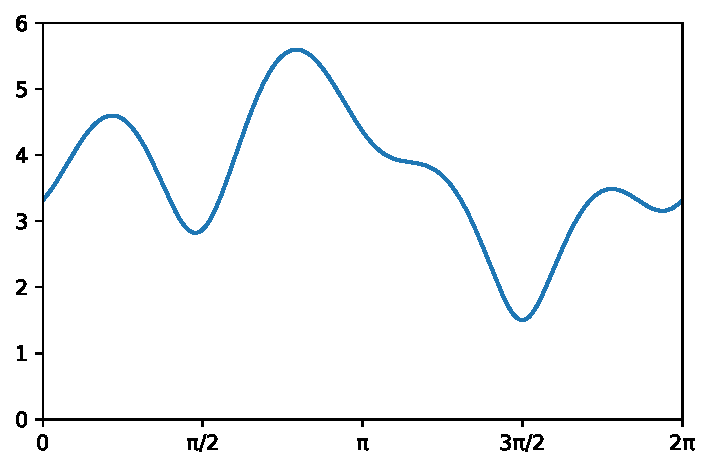
\includegraphics{./intro_files/figure-pdf/fig-graphofdistanceproblem-output-1.pdf}

}

\caption{\label{fig-graphofdistanceproblem}Graph der Abstandsfunktion
\(d(t)\).}

\end{figure}

Wir möchten das Minimum der Funktion \(d(t)\) mit Hilfe der Gradient
Descent Methode finden. Dazu müssen wir aber \(d\) ableiten können.

\end{example}

\begin{center}\rule{0.5\linewidth}{0.5pt}\end{center}

\bookmarksetup{startatroot}

\hypertarget{sec-ADisnot}{%
\chapter{AD ist nicht \ldots{}}\label{sec-ADisnot}}

Bevor wir uns mit den konkreten Implementationen von algorithmischer
Differentiation beschäftigen, wollen wir herausstellen, was AD
\emph{nicht} ist.

\hypertarget{sec-ADnotNumDiff}{%
\section{AD ist nicht numerisches Ableiten}\label{sec-ADnotNumDiff}}

Eine Funktion \(y = f(x)\) ist bekanntlich differenzierbar an der Stelle
\(x_0 \in \mathbb{D}\), wenn der Grenzwert
\[ \lim_{h\rightarrow 0} \frac{f(x_0 + h) - f(x_0)}{h} \] existiert. In
dem Fall ist \(f'(x_0)\) einfach der Wert dieses Grenzwerts.

Ein erster Ansatz zur numerischen Berechnung könnte also sein, den
Differenzenquotienten für kleine \(h\) auszuwerten\footnote{Dieser
  Ansatz kann verbessert werden indem man z.B.
  \(f'(x_0) \approx \frac{f(x_0 + h) - f(x_0 - h)}{2h}\) verwendet. Die
  im Beispiel beschriebenen Probleme bleiben aber auch dann bestehen.}.

\leavevmode\vadjust pre{\hypertarget{exm-numDiff}{}}%
\begin{example}[Numerische Ableitung]\label{exm-numDiff}

Leite die Funktion \(f(x) = x^2\) an der Stelle \(x_0 = 2\) ab.

\begin{Shaded}
\begin{Highlighting}[]
\KeywordTok{def}\NormalTok{ f(x):}
\NormalTok{    y }\OperatorTok{=}\NormalTok{ x }\OperatorTok{**} \DecValTok{2}
    \ControlFlowTok{return}\NormalTok{ y}

\KeywordTok{def}\NormalTok{ fdot(f, x0, h):}
\NormalTok{    df }\OperatorTok{=}\NormalTok{ (f(x0 }\OperatorTok{+}\NormalTok{ h) }\OperatorTok{{-}}\NormalTok{ f(x0)) }\OperatorTok{/}\NormalTok{ h}
    \ControlFlowTok{return}\NormalTok{ df}

\NormalTok{x0 }\OperatorTok{=} \FloatTok{0.2}
\NormalTok{H }\OperatorTok{=}\NormalTok{ [}\FloatTok{0.1}\NormalTok{, }\FloatTok{0.01}\NormalTok{, }\FloatTok{0.001}\NormalTok{, }\FloatTok{0.0001}\NormalTok{]}
\ControlFlowTok{for}\NormalTok{ h }\KeywordTok{in}\NormalTok{ H:}
\NormalTok{    ydot }\OperatorTok{=}\NormalTok{ fdot(f, x0, h)}
    \BuiltInTok{print}\NormalTok{(}\StringTok{"h = "} \OperatorTok{+} \BuiltInTok{str}\NormalTok{(h) }\OperatorTok{+} \StringTok{" }\CharTok{\textbackslash{}t}\StringTok{=\textgreater{} f\textquotesingle{}(x0) = "} \OperatorTok{+} \BuiltInTok{str}\NormalTok{(ydot))}
\end{Highlighting}
\end{Shaded}

\begin{verbatim}
h = 0.1     => f'(x0) = 0.5000000000000001
h = 0.01    => f'(x0) = 0.4099999999999999
h = 0.001   => f'(x0) = 0.4009999999999986
h = 0.0001  => f'(x0) = 0.40009999999993107
\end{verbatim}

Es scheint zunächst, als ob die Werte für kleiner werdende \(h\) zum
korrekten Wert \(f'(0.2)=0.4\) konvergieren. Wenn wir aber an sehr
genauen Werten interessiert sind und entsprechend \(h\) sehr klein
wählen, beobachten wir folgendes:

\begin{Shaded}
\begin{Highlighting}[]
\KeywordTok{def}\NormalTok{ f(x):}
\NormalTok{    y }\OperatorTok{=}\NormalTok{ x }\OperatorTok{**} \DecValTok{2}
    \ControlFlowTok{return}\NormalTok{ y}

\KeywordTok{def}\NormalTok{ fdot(f, x0, h):}
\NormalTok{    df }\OperatorTok{=}\NormalTok{ (f(x0 }\OperatorTok{+}\NormalTok{ h) }\OperatorTok{{-}}\NormalTok{ f(x0)) }\OperatorTok{/}\NormalTok{ h}
    \ControlFlowTok{return}\NormalTok{ df}

\NormalTok{x0 }\OperatorTok{=} \FloatTok{0.2}
\NormalTok{H }\OperatorTok{=}\NormalTok{ [}\DecValTok{10} \OperatorTok{**} \OperatorTok{{-}}\DecValTok{8}\NormalTok{, }\DecValTok{10} \OperatorTok{**} \OperatorTok{{-}}\DecValTok{9}\NormalTok{, }\DecValTok{10} \OperatorTok{**} \OperatorTok{{-}}\DecValTok{10}\NormalTok{, }\DecValTok{10} \OperatorTok{**} \OperatorTok{{-}}\DecValTok{11}\NormalTok{]}
\ControlFlowTok{for}\NormalTok{ h }\KeywordTok{in}\NormalTok{ H:}
\NormalTok{    ydot }\OperatorTok{=}\NormalTok{ fdot(f, x0, h)}
    \BuiltInTok{print}\NormalTok{(}\StringTok{"h = "} \OperatorTok{+} \BuiltInTok{str}\NormalTok{(h) }\OperatorTok{+} \StringTok{"}\CharTok{\textbackslash{}t}\StringTok{=\textgreater{} f\textquotesingle{}(x0) = "} \OperatorTok{+} \BuiltInTok{str}\NormalTok{(ydot))}
\end{Highlighting}
\end{Shaded}

\begin{verbatim}
h = 1e-08   => f'(x0) = 0.4000000095039091
h = 1e-09   => f'(x0) = 0.3999999984016789
h = 1e-10   => f'(x0) = 0.4000000330961484
h = 1e-11   => f'(x0) = 0.3999994779846361
\end{verbatim}

Mit kleiner werdendem \(h\) scheint sich der Näherungswert für die
Ableitung zu verschlechtern. Das Phänomen wird noch deutlicher, wenn wir
den Fehler \(E(h) = \lvert\frac{f(x_0+h)-f(x_0)}{h} - f'(x_0)\rvert\)
als Funktion von \(h\) plotten. Beachte die doppelt logarithmische
Skala.

\begin{Shaded}
\begin{Highlighting}[]
\ImportTok{import}\NormalTok{ matplotlib.pyplot }\ImportTok{as}\NormalTok{ plt}
\ImportTok{import}\NormalTok{ math}

\KeywordTok{def}\NormalTok{ f(x):}
\NormalTok{    y }\OperatorTok{=}\NormalTok{ x }\OperatorTok{**} \DecValTok{2}
    \ControlFlowTok{return}\NormalTok{ y}

\KeywordTok{def}\NormalTok{ fdot(f, x0, h):}
\NormalTok{    df }\OperatorTok{=}\NormalTok{ (f(x0 }\OperatorTok{+}\NormalTok{ h) }\OperatorTok{{-}}\NormalTok{ f(x0)) }\OperatorTok{/}\NormalTok{ h}
    \ControlFlowTok{return}\NormalTok{ df}

\NormalTok{x0 }\OperatorTok{=} \FloatTok{0.2}
\NormalTok{H }\OperatorTok{=}\NormalTok{ [}\DecValTok{10}\OperatorTok{**}\NormalTok{(k}\OperatorTok{/}\DecValTok{100}\NormalTok{) }\ControlFlowTok{for}\NormalTok{ k }\KeywordTok{in} \BuiltInTok{range}\NormalTok{(}\OperatorTok{{-}}\DecValTok{1800}\NormalTok{, }\OperatorTok{{-}}\DecValTok{300}\NormalTok{)]}
\NormalTok{E }\OperatorTok{=}\NormalTok{ [math.fabs(fdot(f, x0, h) }\OperatorTok{{-}} \DecValTok{2}\OperatorTok{*}\NormalTok{x0) }\ControlFlowTok{for}\NormalTok{ h }\KeywordTok{in}\NormalTok{ H]}

\CommentTok{\# Plot}
\NormalTok{fig }\OperatorTok{=}\NormalTok{ plt.figure()}
\NormalTok{ax }\OperatorTok{=}\NormalTok{ fig.add\_axes([}\FloatTok{0.1}\NormalTok{, }\FloatTok{0.1}\NormalTok{, }\FloatTok{0.8}\NormalTok{, }\FloatTok{0.8}\NormalTok{])}
\NormalTok{ax.}\BuiltInTok{set}\NormalTok{(xlim}\OperatorTok{=}\NormalTok{(}\DecValTok{10}\OperatorTok{**{-}}\DecValTok{18}\NormalTok{, }\DecValTok{10}\OperatorTok{**{-}}\DecValTok{3}\NormalTok{), ylim}\OperatorTok{=}\NormalTok{(}\DecValTok{10}\OperatorTok{**{-}}\DecValTok{12}\NormalTok{, }\DecValTok{10}\OperatorTok{**}\DecValTok{0}\NormalTok{))}
\NormalTok{ax.set\_xscale(}\StringTok{\textquotesingle{}log\textquotesingle{}}\NormalTok{)}
\NormalTok{ax.set\_xlabel(}\StringTok{\textquotesingle{}h\textquotesingle{}}\NormalTok{)}
\NormalTok{ax.set\_yscale(}\StringTok{\textquotesingle{}log\textquotesingle{}}\NormalTok{)}
\NormalTok{ax.set\_ylabel(}\StringTok{\textquotesingle{}Fehler E(h)\textquotesingle{}}\NormalTok{)}
\NormalTok{plt.plot(H,E)}
\NormalTok{plt.show()}
\end{Highlighting}
\end{Shaded}

\begin{figure}[H]

{\centering 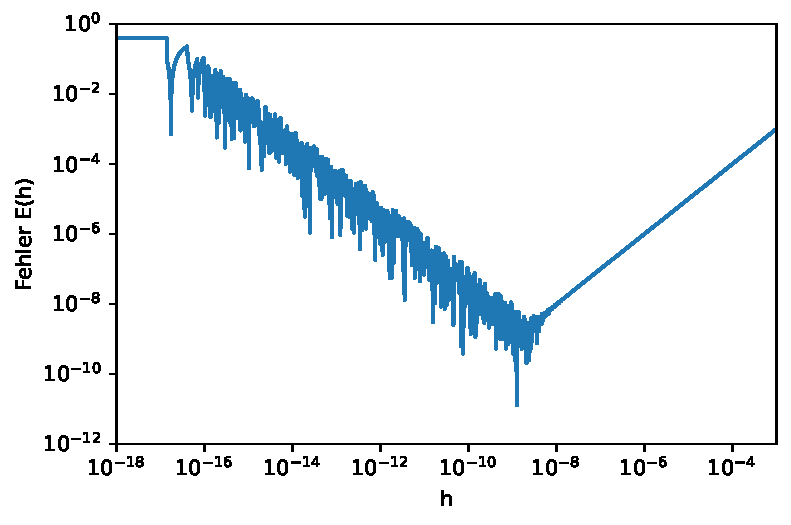
\includegraphics{./notAD_files/figure-pdf/fig-numdiffproblem-output-1.pdf}

}

\caption{\label{fig-numdiffproblem}Grösse des Fehlers \(E(h)\) als
Funktion der Schrittweite \(h\). Ist \(h\) zu gross, dann ist der
Näherungswert für \(f'(x_0)\) ungenau. Bei kleiner werdendem \(h\) nimmt
der Fehler zunächst ab, aber ab einem gewissen Wert dominiert die
Auslöschung und der Fehler nimmt wieder zu.}

\end{figure}

\end{example}

\begin{center}\rule{0.5\linewidth}{0.5pt}\end{center}

\hypertarget{ausluxf6schung}{%
\subsection{Auslöschung}\label{ausluxf6schung}}

Im vorherigen Beispiel haben wir das Phänomen der
\href{https://de.wikipedia.org/wiki/Ausl\%C3\%B6schung_(numerische_Mathematik)}{Auslöschung}
beobachtet. Zunächst ist dir sicher aufgefallen, dass der Näherungswert
für \(f'(x_0)\) mit \(h=0.01\) nicht
\[ \frac{f(x_0 + h) - f(x_0)}{h} = \frac{0.21^2 - 0.2^2}{0.01}=0.41\]
ergab, sondern \(f'(x_0)\approx 0.40999...\). Das liegt daran, dass
Dezimalzahlen nicht exakt als Binärzahl dargestellt werden können. Da
nun die Werte von \(f(x_0 + h)\) und \(f(x_0)\) für kleine \(h\) fast
gleich sind, besteht ihre Differenz \(f(x_0 + h) - f(x_0)\) nur noch aus
diesen Rundungsfehlern. Diese (sinnlose) Differenz ist zwar sehr klein,
wird aber im nächsten Schritt mit der sehr grossen Zahl \(\frac{1}{h}\)
multipliziert, wodurch die Rundungsfehler die gleiche Grössenordnung
annehmen, wie die ursprünglichen Funktionswerte. Mehr über
Rundungsfehler und Auslöschung kann in Weitz (2021) ab S. 117
nachgelesen werden.

\hypertarget{sec-ADnotSymbDiff}{%
\section{AD ist nicht symbolisches Ableiten}\label{sec-ADnotSymbDiff}}

Computer Algebra Systeme (CAS) sind Programme zur Bearbeitung
algebraischer Ausdrücke. Mit solchen Programmen lassen sich auch
Ableitungen symbolisch bestimmen. Wie das funktioniert, wird in Slater
(2022) kurz angedeutet. Bekannte Beispiele für CAS sind etwa
\href{https://www.wolframalpha.com/}{Wolfram Alpha},
\href{https://maxima.sourceforge.io/download.html}{Maxima} oder
\href{https://www.sagemath.org/}{Sage}. Letzteres kann man
\href{https://sagecell.sagemath.org/}{hier} auch online ausprobieren.
Gib z.B. den folgenden Code ein, welcher die Ableitung der Funktion aus
Übungsaufgabe~\ref{exr-LoopProgToFun} bestimmt:

\begin{verbatim}
l(x) = x^2 + 1
f(x) = l(l(l(x)))
fdot = diff(f,x)
expand(fdot)
\end{verbatim}

\begin{tcolorbox}[enhanced jigsaw, title=\textcolor{quarto-callout-tip-color}{\faLightbulb}\hspace{0.5em}{Tipp}, colbacktitle=quarto-callout-tip-color!10!white, bottomrule=.15mm, titlerule=0mm, colback=white, breakable, colframe=quarto-callout-tip-color-frame, bottomtitle=1mm, toptitle=1mm, leftrule=.75mm, arc=.35mm, left=2mm, rightrule=.15mm, toprule=.15mm, opacitybacktitle=0.6, opacityback=0, coltitle=black]
Auf der Website kannst du rechts unter \texttt{Language} auch
\texttt{Maxima} auswählen und Maxima-Code ausführen. Maxima ist in Sage
integriert.
\end{tcolorbox}

Für Python gibt es die Bibliothek \texttt{sympy}, die ein CAS für Python
zur Verfügung stellt. Damit können wir die Funktion aus
Übungsaufgabe~\ref{exr-LoopProgToFun} direkt in Python ableiten:

\leavevmode\vadjust pre{\hypertarget{exm-symbDiff}{}}%
\begin{example}[Symbolische Ableitung]\label{exm-symbDiff}

Leite die Funktion \(f(x) = l(l(l(x)))\), wobei \(l(x) = x^2 + 1\) ist,
an der Stelle \(x_0 = 1\) ab.

\begin{Shaded}
\begin{Highlighting}[]
\ImportTok{from}\NormalTok{ sympy  }\ImportTok{import}\NormalTok{ symbols, diff}

\KeywordTok{def}\NormalTok{ f(x):}
\NormalTok{    v0 }\OperatorTok{=}\NormalTok{ x}
\NormalTok{    v1 }\OperatorTok{=}\NormalTok{ v0 }\OperatorTok{**} \DecValTok{2} \OperatorTok{+} \DecValTok{1}
\NormalTok{    v2 }\OperatorTok{=}\NormalTok{ v1 }\OperatorTok{**} \DecValTok{2} \OperatorTok{+} \DecValTok{1}
\NormalTok{    v3 }\OperatorTok{=}\NormalTok{ v2 }\OperatorTok{**} \DecValTok{2} \OperatorTok{+} \DecValTok{1}
\NormalTok{    y }\OperatorTok{=}\NormalTok{ v3}
    \ControlFlowTok{return}\NormalTok{ y}

\NormalTok{x }\OperatorTok{=}\NormalTok{ symbols(}\StringTok{\textquotesingle{}x\textquotesingle{}}\NormalTok{)}
\BuiltInTok{print}\NormalTok{(}\StringTok{"f(x) ="}\NormalTok{, f(x))}

\NormalTok{df }\OperatorTok{=}\NormalTok{ diff(f(x),x)}
\BuiltInTok{print}\NormalTok{(}\StringTok{"f\textquotesingle{}(x) ="}\NormalTok{, df)}

\NormalTok{x0 }\OperatorTok{=} \DecValTok{1}
\BuiltInTok{print}\NormalTok{(}\StringTok{"f\textquotesingle{}("} \OperatorTok{+} \BuiltInTok{str}\NormalTok{(x0) }\OperatorTok{+} \StringTok{") ="}\NormalTok{, df.evalf(subs}\OperatorTok{=}\NormalTok{\{x:x0\}))}
\end{Highlighting}
\end{Shaded}

\begin{verbatim}
f(x) = ((x**2 + 1)**2 + 1)**2 + 1
f'(x) = 8*x*(x**2 + 1)*((x**2 + 1)**2 + 1)
f'(1) = 80.0000000000000
\end{verbatim}

\end{example}

\begin{center}\rule{0.5\linewidth}{0.5pt}\end{center}

Damit erhält man die (bis auf Maschinengenauigkeit) exakten Werte der
Ableitungen. Der Grund, warum wir nicht auf symbolische Ausdrücke für
Ableitungen zurückgreifen wollen, liegt darin, dass diese Methode bei
komplizierten Funktionsausdrücken sehr ineffizient ist, insbesondere
dann, wenn wir auch Ableitungen von Funktionen
\(f : \mathbb{R}^n \rightarrow \mathbb{R}^m\) berechnen wollen.

\bookmarksetup{startatroot}

\hypertarget{sec-SADforOneDimFunctions}{%
\chapter{Standard Algorithmische Differentiation für eindimensionale
Funktionen}\label{sec-SADforOneDimFunctions}}

In Kapitel~\ref{sec-ADisnot} haben wir zwei Methoden für die Berechnung
von Ableitungen kennen gelernt, die beide ihre Schwächen haben. Während
die numerische Ableitung mit geringem Aufwand berechnet werden kann,
sind ihre Näherungswerte für viele Anwendungen zu ungenau. Symbolische
Ableitungen andererseits liefern zwar exakte Werte von Ableitungen, sind
aber mit grossem Rechenaufwand verbunden. Die hier vorgestellte
Algorithmische Differentiation (AD) vereinigt die Vorteile der beiden
Methoden. Sie liefert uns (bis auf Maschinengenauigkeit) exakte Werte
von Ableitungen mit nur einem geringen zusätzlichen Rechenaufwand:

\begin{quote}
``AD as a technical term refers to a specific family of techniques that
compute derivatives trhough accumulation of values during code execution
to generate numerical derivative evaluations rather than derivative
expressions. This allows accurate evaluation of derivatives at machine
precision with only a small constant factor of overhead and ideal
asymptotic efficiency.'' (Baydin u.~a. (2018), S. 2)
\end{quote}

In diesem Kapitel lernen wir die \emph{Standard Algorithmische
Differentiation} (SAD, auch Vorwärts-AD genannt) kennen, welche die
einfachste Variante der erwähnten ``family of techniques'' ist. Wir
beschränken uns zunächst wieder auf Funktionen
\(f : \mathbb{R} \rightarrow \mathbb{R}\) und werden dies später auf
Funktionen \(f : \mathbb{R}^n \rightarrow \mathbb{R}^m\) erweitern.
Neben der Standard-AD gibt es noch die \emph{Adjungierte Algorithmische
Differentiation} (AAD, auch Rückwärts-AD genannt). Die Vorteile dieser
Methode offenbaren sich jedoch erst für Funktionen in höherdimensionalen
Räumen.

Gemäss unserer Konvention in Kapitel~\ref{sec-ProgFunc} berechnen wir
eine mathematische Funktion, indem wir sie in ihre Bestandteile
zerlegen, und die Zwischenergebnisse Variablen \texttt{v} zuweisen. Wie
im obigen Zitat erwähnt, besteht die Grundidee der AD darin, eine Reihe
von Hilfsvariablen \texttt{vdot} einzuführen, welche jeweils die Werte
der Ableitungen enthalten. In diesem Kapitel machen wir dies explizit,
indem wir jede Programmzeile, die ein \texttt{v} berechnet, um die
Berechnung des zugehörigen \texttt{vdot} erweitern. Dies scheint
zunächst umständlich zu sein, aber im nächsten Abschnitt werden wir eine
Klasse schreiben, die diese Schritte für uns automatisiert. Wie Marc
Henrard in seinem Buch schreibt:

\begin{quote}
``There are as many shades of AD as there are AD users. {[}This
chapter{]} provides to the user the black and the white; it is up to him
to get the correct shade of grey that fits his taste and his
requirements.'' (Henrard (2017), S. 18)
\end{quote}

\hypertarget{sec-SadManualImplementation}{%
\section{Manuelle Implementation der
SAD}\label{sec-SadManualImplementation}}

Beginnen wir mit einem Beispiel:

Wir möchten den Funktionswert und die Ableitung der Funktion
\(y=f(x)=\sin(x^2)\) an der Stelle \(x_0=\frac{\pi}{2}\) bestimmen. Das
folgende Programm berechnet den Funktionswert.

\begin{Shaded}
\begin{Highlighting}[]
\ImportTok{import}\NormalTok{ math}

\KeywordTok{def}\NormalTok{ f(x):}
\NormalTok{    v0 }\OperatorTok{=}\NormalTok{ x}
\NormalTok{    v1 }\OperatorTok{=}\NormalTok{ v0}\OperatorTok{**}\DecValTok{2}
\NormalTok{    v2 }\OperatorTok{=}\NormalTok{ math.sin(v1)}
\NormalTok{    y }\OperatorTok{=}\NormalTok{ v2}
    \ControlFlowTok{return}\NormalTok{ y}

\NormalTok{x0 }\OperatorTok{=}\NormalTok{ math.pi }\OperatorTok{/} \DecValTok{2}
\BuiltInTok{print}\NormalTok{(f(x0))}
\end{Highlighting}
\end{Shaded}

\begin{verbatim}
0.6242659526396992
\end{verbatim}

\(f\) ist eine zusammengesetzte Funktion, die wir mit den Funktionen \[
\begin{flalign}
    v_0(x)   &= x \\
    v_1(v_0) &= v_0 ^2 \\
    v_2(v_1) &= \sin(v_1)
\end{flalign}
\] schreiben können als \(y=f(x)=v_2(v_1(v_0(x)))\). Die Ableitung
berechnet sich dann mit der Kettenregel zu \[
f'(x) = \frac{dv_2}{dv_1} \cdot \frac{dv_1}{dv_0} \cdot \frac{dv_0}{dx} = \cos(v_1)\cdot 2v_0 \cdot 1 = \cos(x^2) \cdot 2x \cdot 1
\] Wir können also die Ableitung von \texttt{f(x)} berechnen, indem wir
jede Zeile des Programms gemäss den bekannten Regeln ableiten:

\begin{verbatim}
v0dot = 1
v1dot = 2 * v0 * v0dot
v2dot = math.cos(v1) * v1dot
\end{verbatim}

Man beachte, dass durch die Konvention, dass immer \texttt{v0\ =\ x}
gesetzt wird, auch immer \texttt{v0dot\ =\ 1} ist. Nun können wir unsere
Funktion so ergänzen, dass nicht nur der Funktionswert, sondern auch die
Ableitung an der Stelle \(x_0\) berechnet wird:

\begin{Shaded}
\begin{Highlighting}[]
\ImportTok{import}\NormalTok{ math}

\KeywordTok{def}\NormalTok{ f(x):}
\NormalTok{    v0dot }\OperatorTok{=} \DecValTok{1}
\NormalTok{    v0 }\OperatorTok{=}\NormalTok{ x}
\NormalTok{    v1dot }\OperatorTok{=} \DecValTok{2} \OperatorTok{*}\NormalTok{ v0 }\OperatorTok{*}\NormalTok{ v0dot}
\NormalTok{    v1 }\OperatorTok{=}\NormalTok{ v0}\OperatorTok{**}\DecValTok{2}
\NormalTok{    v2dot }\OperatorTok{=}\NormalTok{ math.cos(v1) }\OperatorTok{*}\NormalTok{ v1dot}
\NormalTok{    v2 }\OperatorTok{=}\NormalTok{ math.sin(v1)}
\NormalTok{    ydot }\OperatorTok{=}\NormalTok{ v2dot}
\NormalTok{    y }\OperatorTok{=}\NormalTok{ v2}
    \ControlFlowTok{return}\NormalTok{ [y, ydot]}

\NormalTok{x0 }\OperatorTok{=}\NormalTok{ math.pi }\OperatorTok{/} \DecValTok{2}
\BuiltInTok{print}\NormalTok{(f(x0))}
\end{Highlighting}
\end{Shaded}

\begin{verbatim}
[0.6242659526396992, -2.4542495411512917]
\end{verbatim}

Die Korrektheit des Programms können wir mit
\href{https://www.geogebra.org/m/u4rkpzsr}{GeoGebra} überprüfen, welches
Ableitungen symbolisch berechnet.

Beachte, dass wir konsequent die Kettenregel verwendet haben. So wird
aus \texttt{v1\ =\ v0**2} etwa \texttt{v1dot\ =\ 2\ *\ v0\ *\ v0dot}
oder aus \texttt{v2\ =\ sin(v1)} wird
\texttt{v2dot\ =\ cos(v1)\ *\ v1dot}.

\leavevmode\vadjust pre{\hypertarget{exr-ErstesADBspErweitern}{}}%
\begin{exercise}[Programm ableiten]\label{exr-ErstesADBspErweitern}

Ändere das vorherige Programm so ab, dass der Funktionswert und die
Ableitung der Funktion \(y = f(x) = \ln(\sin(x^2))\) an der Stelle
\(x_0 = \frac{\pi}{2}\) berechnet wird. Überprüfe deine Lösung mit
GeoGebra.

\end{exercise}

\begin{tcolorbox}[enhanced jigsaw, title=\textcolor{quarto-callout-tip-color}{\faLightbulb}\hspace{0.5em}{Lösung}, colbacktitle=quarto-callout-tip-color!10!white, bottomrule=.15mm, titlerule=0mm, colback=white, breakable, colframe=quarto-callout-tip-color-frame, bottomtitle=1mm, toptitle=1mm, leftrule=.75mm, arc=.35mm, left=2mm, rightrule=.15mm, toprule=.15mm, opacitybacktitle=0.6, opacityback=0, coltitle=black]

Es müssen lediglich zwei weitere Zeilen eingefügt werden und zwar für
die Berechnung von \texttt{v3} und \texttt{v3dot}. Vergiss nicht, die
richtigen Werte zurückzugeben.

\begin{Shaded}
\begin{Highlighting}[]
\ImportTok{import}\NormalTok{ math}

\KeywordTok{def}\NormalTok{ f(x):}
\NormalTok{    v0dot }\OperatorTok{=} \DecValTok{1}
\NormalTok{    v0 }\OperatorTok{=}\NormalTok{ x}
\NormalTok{    v1dot }\OperatorTok{=} \DecValTok{2} \OperatorTok{*}\NormalTok{ v0 }\OperatorTok{*}\NormalTok{ v0dot}
\NormalTok{    v1 }\OperatorTok{=}\NormalTok{ v0}\OperatorTok{**}\DecValTok{2}
\NormalTok{    v2dot }\OperatorTok{=}\NormalTok{ math.cos(v1) }\OperatorTok{*}\NormalTok{ v1dot}
\NormalTok{    v2 }\OperatorTok{=}\NormalTok{ math.sin(v1)}
\NormalTok{    v3dot }\OperatorTok{=} \DecValTok{1} \OperatorTok{/}\NormalTok{ v2 }\OperatorTok{*}\NormalTok{ v2dot}
\NormalTok{    v3 }\OperatorTok{=}\NormalTok{ math.log(v2)}
\NormalTok{    ydot }\OperatorTok{=}\NormalTok{ v3dot}
\NormalTok{    y }\OperatorTok{=}\NormalTok{ v3}
    \ControlFlowTok{return}\NormalTok{ [y, ydot]}

\NormalTok{x0 }\OperatorTok{=}\NormalTok{ math.pi }\OperatorTok{/} \DecValTok{2}
\BuiltInTok{print}\NormalTok{(f(x0))}
\end{Highlighting}
\end{Shaded}

\begin{verbatim}
[-0.4711787952593891, -3.9314166194288416]
\end{verbatim}

\end{tcolorbox}

\begin{tcolorbox}[enhanced jigsaw, title=\textcolor{quarto-callout-important-color}{\faExclamation}\hspace{0.5em}{Konvention}, colbacktitle=quarto-callout-important-color!10!white, bottomrule=.15mm, titlerule=0mm, colback=white, breakable, colframe=quarto-callout-important-color-frame, bottomtitle=1mm, toptitle=1mm, leftrule=.75mm, arc=.35mm, left=2mm, rightrule=.15mm, toprule=.15mm, opacitybacktitle=0.6, opacityback=0, coltitle=black]

Ein Programm, welches gemäss der Konvention in
Kapitel~\ref{sec-ProgFunc} geschrieben ist, wird folgendermassen
abgeleitet:

\begin{enumerate}
\def\labelenumi{\arabic{enumi}.}
\tightlist
\item
  Für jede Variable \texttt{v} wird eine neue Variable \texttt{vdot} für
  den Wert der Ableitung definiert, angefangen bei \texttt{v0dot\ =\ 1}.
\item
  Jede Programmzeile wird gemäss den bekannten Regeln aus
  Tabelle~\ref{tbl-DiffGrundfunktionen} und Tabelle~\ref{tbl-DiffRegeln}
  abgeleitet. Dabei wird insbesondere in \emph{jeder} Zeile die
  Kettenregel verwendet.
\item
  Die abgeleitete Anweisung wird jeweils \emph{vor} (!) die zu
  ableitende Anweisung eingeschoben.
\end{enumerate}

\end{tcolorbox}

\leavevmode\vadjust pre{\hypertarget{exr-SADProduktregel}{}}%
\begin{exercise}[Produktregel]\label{exr-SADProduktregel}

Das folgende Programm berechnet die Funktion \(y = f(x) = (2+x)(x-3)\):

\begin{Shaded}
\begin{Highlighting}[]
\KeywordTok{def}\NormalTok{ f(x):}
\NormalTok{    v0 }\OperatorTok{=}\NormalTok{ x}
\NormalTok{    v1 }\OperatorTok{=} \DecValTok{2} \OperatorTok{+}\NormalTok{ v0}
\NormalTok{    v2 }\OperatorTok{=}\NormalTok{ v0 }\OperatorTok{{-}} \DecValTok{3}
\NormalTok{    y }\OperatorTok{=}\NormalTok{ v1 }\OperatorTok{*}\NormalTok{ v2}
    \ControlFlowTok{return}\NormalTok{ y}
\end{Highlighting}
\end{Shaded}

Leite dieses Programm ab. Dein Programm soll die Gleichung der Tangente
\(t(x) = f(x_0) + f'(x_0)\cdot (x-x_0)\) an der Stelle \(x_0 = 2\)
ausgeben.

\end{exercise}

\begin{tcolorbox}[enhanced jigsaw, title=\textcolor{quarto-callout-tip-color}{\faLightbulb}\hspace{0.5em}{Lösung}, colbacktitle=quarto-callout-tip-color!10!white, bottomrule=.15mm, titlerule=0mm, colback=white, breakable, colframe=quarto-callout-tip-color-frame, bottomtitle=1mm, toptitle=1mm, leftrule=.75mm, arc=.35mm, left=2mm, rightrule=.15mm, toprule=.15mm, opacitybacktitle=0.6, opacityback=0, coltitle=black]

\begin{Shaded}
\begin{Highlighting}[]
\KeywordTok{def}\NormalTok{ f(x):}
\NormalTok{    v0dot }\OperatorTok{=} \DecValTok{1}
\NormalTok{    v0 }\OperatorTok{=}\NormalTok{ x}
\NormalTok{    v1dot }\OperatorTok{=}\NormalTok{ v0dot}
\NormalTok{    v1 }\OperatorTok{=} \DecValTok{2} \OperatorTok{+}\NormalTok{ v0}
\NormalTok{    v2dot }\OperatorTok{=}\NormalTok{ v0dot}
\NormalTok{    v2 }\OperatorTok{=}\NormalTok{ v0 }\OperatorTok{{-}} \DecValTok{3}
\NormalTok{    ydot }\OperatorTok{=}\NormalTok{ v1dot }\OperatorTok{*}\NormalTok{ v2 }\OperatorTok{+}\NormalTok{ v1 }\OperatorTok{*}\NormalTok{ v2dot }\CommentTok{\# Produktregel}
\NormalTok{    y }\OperatorTok{=}\NormalTok{ v1 }\OperatorTok{*}\NormalTok{ v2}
    \ControlFlowTok{return}\NormalTok{ [y, ydot]}

\NormalTok{x0 }\OperatorTok{=} \DecValTok{2}
\NormalTok{[y0, y0dot] }\OperatorTok{=}\NormalTok{ f(x0)}
\BuiltInTok{print}\NormalTok{(}\StringTok{"t(x) ="}\NormalTok{, y0, }\StringTok{"+"}\NormalTok{, y0dot, }\StringTok{"* ( x {-}"}\NormalTok{, x0, }\StringTok{")"}\NormalTok{)}
\end{Highlighting}
\end{Shaded}

\begin{verbatim}
t(x) = -4 + 3 * ( x - 2 )
\end{verbatim}

\end{tcolorbox}

\leavevmode\vadjust pre{\hypertarget{exr-SAD1}{}}%
\begin{exercise}[Programm ableiten]\label{exr-SAD1}

Leite die Funktion aus Übungsaufgabe~\ref{exr-ProgToFun} ab. Gib den
Funktionswert und den Wert der Ableitung an der Stelle \(x_0=-2\) aus.

\end{exercise}

\begin{tcolorbox}[enhanced jigsaw, title=\textcolor{quarto-callout-tip-color}{\faLightbulb}\hspace{0.5em}{Lösung}, colbacktitle=quarto-callout-tip-color!10!white, bottomrule=.15mm, titlerule=0mm, colback=white, breakable, colframe=quarto-callout-tip-color-frame, bottomtitle=1mm, toptitle=1mm, leftrule=.75mm, arc=.35mm, left=2mm, rightrule=.15mm, toprule=.15mm, opacitybacktitle=0.6, opacityback=0, coltitle=black]

\begin{Shaded}
\begin{Highlighting}[]
\ImportTok{import}\NormalTok{ math}

\KeywordTok{def}\NormalTok{ f(x):}
\NormalTok{    v0dot }\OperatorTok{=} \DecValTok{1}
\NormalTok{    v0 }\OperatorTok{=}\NormalTok{ x}
\NormalTok{    v1dot }\OperatorTok{=} \DecValTok{2} \OperatorTok{*}\NormalTok{ v0 }\OperatorTok{*}\NormalTok{ v0dot}
\NormalTok{    v1 }\OperatorTok{=}\NormalTok{ v0 }\OperatorTok{**} \DecValTok{2}
\NormalTok{    v2dot }\OperatorTok{=}\NormalTok{ v1dot}
\NormalTok{    v2 }\OperatorTok{=}\NormalTok{ v1 }\OperatorTok{+} \DecValTok{2}
\NormalTok{    v3dot }\OperatorTok{=} \OperatorTok{{-}}\DecValTok{1}\OperatorTok{/}\DecValTok{2} \OperatorTok{*}\NormalTok{ v1dot}
\NormalTok{    v3 }\OperatorTok{=} \OperatorTok{{-}}\NormalTok{v1 }\OperatorTok{/} \DecValTok{2}
\NormalTok{    v4dot }\OperatorTok{=} \OperatorTok{{-}}\NormalTok{math.sin(v2) }\OperatorTok{*}\NormalTok{ v2dot}
\NormalTok{    v4 }\OperatorTok{=}\NormalTok{ math.cos(v2)}
\NormalTok{    v5dot }\OperatorTok{=}\NormalTok{ math.exp(v3) }\OperatorTok{*}\NormalTok{ v3dot}
\NormalTok{    v5 }\OperatorTok{=}\NormalTok{ math.exp(v3)}
\NormalTok{    v6dot }\OperatorTok{=}\NormalTok{ v4dot }\OperatorTok{*}\NormalTok{ v5 }\OperatorTok{+}\NormalTok{ v4 }\OperatorTok{*}\NormalTok{ v5dot}
\NormalTok{    v6 }\OperatorTok{=}\NormalTok{ v4 }\OperatorTok{*}\NormalTok{ v5}
\NormalTok{    ydot }\OperatorTok{=}\NormalTok{ v6dot }\OperatorTok{{-}} \DecValTok{1} \OperatorTok{/}\NormalTok{ v0}\OperatorTok{**}\DecValTok{2} \OperatorTok{*}\NormalTok{ v0dot}
\NormalTok{    y }\OperatorTok{=}\NormalTok{ v6 }\OperatorTok{+} \DecValTok{1} \OperatorTok{/}\NormalTok{ v0}
    \ControlFlowTok{return}\NormalTok{ [y, ydot]}

\NormalTok{x0 }\OperatorTok{=} \OperatorTok{{-}}\DecValTok{2}
\BuiltInTok{print}\NormalTok{(f(x0))}
\end{Highlighting}
\end{Shaded}

\begin{verbatim}
[-0.3700550823007931, -0.14136926695938976]
\end{verbatim}

\end{tcolorbox}

\leavevmode\vadjust pre{\hypertarget{exr-SAD2}{}}%
\begin{exercise}[Programm ableiten]\label{exr-SAD2}

Leite die Funktion aus Übungsaufgabe~\ref{exr-FunToGraphProg} ab.

\end{exercise}

\begin{tcolorbox}[enhanced jigsaw, title=\textcolor{quarto-callout-tip-color}{\faLightbulb}\hspace{0.5em}{Lösung}, colbacktitle=quarto-callout-tip-color!10!white, bottomrule=.15mm, titlerule=0mm, colback=white, breakable, colframe=quarto-callout-tip-color-frame, bottomtitle=1mm, toptitle=1mm, leftrule=.75mm, arc=.35mm, left=2mm, rightrule=.15mm, toprule=.15mm, opacitybacktitle=0.6, opacityback=0, coltitle=black]

\begin{Shaded}
\begin{Highlighting}[]
\ImportTok{import}\NormalTok{ math}

\KeywordTok{def}\NormalTok{ f(x):}
\NormalTok{    v0dot }\OperatorTok{=} \DecValTok{1}
\NormalTok{    v0 }\OperatorTok{=}\NormalTok{ x}
\NormalTok{    v1dot }\OperatorTok{=} \DecValTok{2} \OperatorTok{*}\NormalTok{ v0 }\OperatorTok{*}\NormalTok{ v0dot}
\NormalTok{    v1 }\OperatorTok{=}\NormalTok{ v0 }\OperatorTok{**} \DecValTok{2}
\NormalTok{    v2dot }\OperatorTok{=}\NormalTok{ v1dot}
\NormalTok{    v2 }\OperatorTok{=}\NormalTok{ v1 }\OperatorTok{+} \DecValTok{1}
\NormalTok{    v3dot }\OperatorTok{=}\NormalTok{ v2dot }\OperatorTok{+}\NormalTok{ v0dot}
\NormalTok{    v3 }\OperatorTok{=}\NormalTok{ v2 }\OperatorTok{+}\NormalTok{ v0}
\NormalTok{    v4dot }\OperatorTok{=} \DecValTok{1} \OperatorTok{/}\NormalTok{ v2 }\OperatorTok{*}\NormalTok{ v2dot}
\NormalTok{    v4 }\OperatorTok{=}\NormalTok{ math.log(v2)}
\NormalTok{    v5dot }\OperatorTok{=} \DecValTok{1} \OperatorTok{/}\NormalTok{ (}\DecValTok{2} \OperatorTok{*}\NormalTok{ math.sqrt(v3)) }\OperatorTok{*}\NormalTok{ v3dot}
\NormalTok{    v5 }\OperatorTok{=}\NormalTok{ math.sqrt(v3)}
\NormalTok{    ydot }\OperatorTok{=}\NormalTok{ (v4dot }\OperatorTok{*}\NormalTok{ v5 }\OperatorTok{{-}}\NormalTok{ v4 }\OperatorTok{*}\NormalTok{ v5dot) }\OperatorTok{/}\NormalTok{ v5}\OperatorTok{**}\DecValTok{2}
\NormalTok{    y }\OperatorTok{=}\NormalTok{ v4 }\OperatorTok{/}\NormalTok{ v5}
    \ControlFlowTok{return}\NormalTok{ [y, ydot]}
\end{Highlighting}
\end{Shaded}

\end{tcolorbox}

Bei all diesen Beispielen könnten wir auch die Reihenfolge der
Anweisungen für \texttt{vdot} und \texttt{v} vertauschen, d.h. zuerst
die Variable \texttt{v} berechnen und erst danach das zugehörige
\texttt{vdot}. Die folgende Übung zeigt aber, warum der 3. Punkt unserer
Konvention wichtig ist.

\leavevmode\vadjust pre{\hypertarget{exr-SADmitSchleife}{}}%
\begin{exercise}[Ein Programm mit einer
Schleife]\label{exr-SADmitSchleife}

Betrachte die Funktion aus Übungsaufgabe~\ref{exr-LoopProgToFun}, welche
aus \(\ell(x) = x^2 + 1\) die Funktion
\(y = f(x) = \ell(\ell(\ell(x)))\) berechnet. Aus
Beispiel~\ref{exm-symbDiff} wissen wir, dass \(f'(1) = 80\) ist.
Vergleiche nun die beiden Varianten für die Ableitung des Programms:

\hypertarget{vdot-vor-v}{%
\subsubsection*{\texorpdfstring{\texttt{vdot} vor
\texttt{v}}{vdot vor v}}\label{vdot-vor-v}}
\addcontentsline{toc}{subsubsection}{\texttt{vdot} vor \texttt{v}}

\begin{Shaded}
\begin{Highlighting}[]
\KeywordTok{def}\NormalTok{ f(x):}
\NormalTok{    v0dot }\OperatorTok{=} \DecValTok{1}
\NormalTok{    v0 }\OperatorTok{=}\NormalTok{ x}
    \ControlFlowTok{for}\NormalTok{ i }\KeywordTok{in} \BuiltInTok{range}\NormalTok{(}\DecValTok{3}\NormalTok{):}
\NormalTok{        v0dot }\OperatorTok{=} \DecValTok{2} \OperatorTok{*}\NormalTok{ v0 }\OperatorTok{*}\NormalTok{ v0dot}
\NormalTok{        v0 }\OperatorTok{=}\NormalTok{ v0 }\OperatorTok{**} \DecValTok{2} \OperatorTok{+} \DecValTok{1}
\NormalTok{    ydot }\OperatorTok{=}\NormalTok{ v0dot}
\NormalTok{    y }\OperatorTok{=}\NormalTok{ v0}
    \ControlFlowTok{return}\NormalTok{ [y, ydot]}

\BuiltInTok{print}\NormalTok{(f(}\DecValTok{1}\NormalTok{))}
\end{Highlighting}
\end{Shaded}

\begin{verbatim}
[26, 80]
\end{verbatim}

\hypertarget{v-vor-vdot}{%
\subsubsection*{\texorpdfstring{\texttt{v} vor
\texttt{vdot}}{v vor vdot}}\label{v-vor-vdot}}
\addcontentsline{toc}{subsubsection}{\texttt{v} vor \texttt{vdot}}

\begin{Shaded}
\begin{Highlighting}[]
\KeywordTok{def}\NormalTok{ f(x):}
\NormalTok{    v0 }\OperatorTok{=}\NormalTok{ x}
\NormalTok{    v0dot }\OperatorTok{=} \DecValTok{1}
    \ControlFlowTok{for}\NormalTok{ i }\KeywordTok{in} \BuiltInTok{range}\NormalTok{(}\DecValTok{3}\NormalTok{):}
\NormalTok{        v0 }\OperatorTok{=}\NormalTok{ v0 }\OperatorTok{**} \DecValTok{2} \OperatorTok{+} \DecValTok{1}
\NormalTok{        v0dot }\OperatorTok{=} \DecValTok{2} \OperatorTok{*}\NormalTok{ v0 }\OperatorTok{*}\NormalTok{ v0dot}
\NormalTok{    y }\OperatorTok{=}\NormalTok{ v0}
\NormalTok{    ydot }\OperatorTok{=}\NormalTok{ v0dot}
    \ControlFlowTok{return}\NormalTok{ [y, ydot]}

\BuiltInTok{print}\NormalTok{(f(}\DecValTok{1}\NormalTok{))}
\end{Highlighting}
\end{Shaded}

\begin{verbatim}
[26, 2080]
\end{verbatim}

Warum wird bei der 2. Variante der Wert der Ableitung falsch berechnet?

\end{exercise}

\begin{tcolorbox}[enhanced jigsaw, title=\textcolor{quarto-callout-tip-color}{\faLightbulb}\hspace{0.5em}{Lösung}, colbacktitle=quarto-callout-tip-color!10!white, bottomrule=.15mm, titlerule=0mm, colback=white, breakable, colframe=quarto-callout-tip-color-frame, bottomtitle=1mm, toptitle=1mm, leftrule=.75mm, arc=.35mm, left=2mm, rightrule=.15mm, toprule=.15mm, opacitybacktitle=0.6, opacityback=0, coltitle=black]
Das Problem tritt in der Schleife auf. In der 2. Variante überschreiben
wir den Wert von \texttt{v0} bereits mit dem neuen Wert der Iteration.
Bei der Berechnung von \texttt{v0dot} hätten wir aber noch den alten
Wert gebraucht. Die Reihenfolge ist also nur in der 1. Version korrekt.
Würden wir die Schleife eliminieren und dafür wie in der Lösung zu
Übungsaufgabe~\ref{exr-LoopProgToFun} für jeden Schleifendurchgang
fortlaufend numerierte Variablen für die \texttt{v} und \texttt{vdot}
verwenden, dann wäre die Reihenfolge wieder egal.
\end{tcolorbox}

In der nächsten Übungsaufgabe verwenden wir die Technik der AD, um das
Billardproblem aus Kapitel~\ref{sec-Newtonverfahren1D} mit dem
Newtonverfahren zu lösen. Da uns die Funktion \texttt{f(x)} nun nicht
mehr nur der Funktionswert, sondern auch die Ableitung berechnet, können
wir das Newtonverfahren ohne die Probleme aus
Übungsaufgabe~\ref{exr-NewtonFirstTry} implementieren.

\leavevmode\vadjust pre{\hypertarget{exr-BillardSADmanualSOlution}{}}%
\begin{exercise}[Das
Billard-Problem]\label{exr-BillardSADmanualSOlution}

Leite das Programm aus Beispiel~\ref{exm-Billard} ab. Schreibe danach
eine Funktion \texttt{newton(f,\ x0)}, welche ausnutzt, dass der
Funktionsaufruf \texttt{f(x0)} auch den exakten Wert der Ableitung
zurückgibt. Stelle alle gefundenen Lösungen grafisch dar.

\end{exercise}

\begin{tcolorbox}[enhanced jigsaw, title=\textcolor{quarto-callout-tip-color}{\faLightbulb}\hspace{0.5em}{Lösung}, colbacktitle=quarto-callout-tip-color!10!white, bottomrule=.15mm, titlerule=0mm, colback=white, breakable, colframe=quarto-callout-tip-color-frame, bottomtitle=1mm, toptitle=1mm, leftrule=.75mm, arc=.35mm, left=2mm, rightrule=.15mm, toprule=.15mm, opacitybacktitle=0.6, opacityback=0, coltitle=black]

\begin{Shaded}
\begin{Highlighting}[]
\ImportTok{import}\NormalTok{ math}
\ImportTok{import}\NormalTok{ matplotlib.pyplot }\ImportTok{as}\NormalTok{ plt}

\KeywordTok{def}\NormalTok{ f(x):}
    \CommentTok{\# Parameter werden im global space gefunden}
    \CommentTok{\# Berechnung des Skalarprodukts und dessen Ableitung}
\NormalTok{    v0dot }\OperatorTok{=} \DecValTok{1}
\NormalTok{    v0 }\OperatorTok{=}\NormalTok{ x}
\NormalTok{    v1dot }\OperatorTok{=} \OperatorTok{{-}}\NormalTok{math.sin(v0) }\OperatorTok{*}\NormalTok{ v0dot  }\CommentTok{\# Ableitung von ...}
\NormalTok{    v1 }\OperatorTok{=}\NormalTok{ math.cos(v0)  }\CommentTok{\# x{-}Koordinate von X}
\NormalTok{    v2dot }\OperatorTok{=}\NormalTok{ math.cos(v0) }\OperatorTok{*}\NormalTok{ v0dot   }\CommentTok{\# Ableitung von ...}
\NormalTok{    v2 }\OperatorTok{=}\NormalTok{ math.sin(v0)  }\CommentTok{\# y{-}Koordinate von X}
\NormalTok{    v3dot }\OperatorTok{=} \OperatorTok{{-}}\NormalTok{ v1dot    }\CommentTok{\# Ableitung von ...}
\NormalTok{    v3 }\OperatorTok{=}\NormalTok{ px }\OperatorTok{{-}}\NormalTok{ v1       }\CommentTok{\# x{-}Komponente des Vektors XP}
\NormalTok{    v4dot }\OperatorTok{=} \OperatorTok{{-}}\NormalTok{ v2dot    }\CommentTok{\# Ableitung von ...}
\NormalTok{    v4 }\OperatorTok{=}\NormalTok{ py }\OperatorTok{{-}}\NormalTok{ v2       }\CommentTok{\# y{-}Komponente des Vektors XP}
\NormalTok{    v5dot }\OperatorTok{=} \DecValTok{1} \OperatorTok{/}\NormalTok{ (}\DecValTok{2}\OperatorTok{*}\NormalTok{math.sqrt(v3}\OperatorTok{**}\DecValTok{2} \OperatorTok{+}\NormalTok{ v4}\OperatorTok{**}\DecValTok{2}\NormalTok{)) }\OperatorTok{\textbackslash{}}
        \OperatorTok{*}\NormalTok{ (}\DecValTok{2}\OperatorTok{*}\NormalTok{v3}\OperatorTok{*}\NormalTok{v3dot }\OperatorTok{+} \DecValTok{2}\OperatorTok{*}\NormalTok{v4}\OperatorTok{*}\NormalTok{v4dot)  }\CommentTok{\# Ableitung von ...}
\NormalTok{    v5 }\OperatorTok{=}\NormalTok{ math.sqrt(v3}\OperatorTok{**}\DecValTok{2} \OperatorTok{+}\NormalTok{ v4}\OperatorTok{**}\DecValTok{2}\NormalTok{)  }\CommentTok{\# Länge des Vektors XP}
\NormalTok{    v6dot }\OperatorTok{=}\NormalTok{ (v3dot }\OperatorTok{*}\NormalTok{ v5 }\OperatorTok{{-}}\NormalTok{ v3 }\OperatorTok{*}\NormalTok{ v5dot) }\OperatorTok{/}\NormalTok{ v5}\OperatorTok{**}\DecValTok{2}  \CommentTok{\# Ableitung von ...}
\NormalTok{    v6 }\OperatorTok{=}\NormalTok{ v3 }\OperatorTok{/}\NormalTok{ v5       }\CommentTok{\# x{-}Komponente des Einheitsvektors eP}
\NormalTok{    v7dot }\OperatorTok{=}\NormalTok{ (v4dot }\OperatorTok{*}\NormalTok{ v5 }\OperatorTok{{-}}\NormalTok{ v4 }\OperatorTok{*}\NormalTok{ v5dot) }\OperatorTok{/}\NormalTok{ v5}\OperatorTok{**}\DecValTok{2}  \CommentTok{\# Ableitung von ...}
\NormalTok{    v7 }\OperatorTok{=}\NormalTok{ v4 }\OperatorTok{/}\NormalTok{ v5       }\CommentTok{\# y{-}Komponente des Einheitsvektors eP}
\NormalTok{    v8dot }\OperatorTok{=} \OperatorTok{{-}}\NormalTok{v1dot     }\CommentTok{\# Ableitung von ...}
\NormalTok{    v8 }\OperatorTok{=}\NormalTok{ a }\OperatorTok{{-}}\NormalTok{ v1        }\CommentTok{\# x{-}Komponente des Vektors XQ}
\NormalTok{    v9dot }\OperatorTok{=} \OperatorTok{{-}}\NormalTok{v2dot     }\CommentTok{\# Ableitung von ...}
\NormalTok{    v9 }\OperatorTok{=} \OperatorTok{{-}}\NormalTok{v2           }\CommentTok{\# y{-}Komponente des Vektors XQ}
\NormalTok{    v10dot }\OperatorTok{=} \DecValTok{1} \OperatorTok{/}\NormalTok{ (}\DecValTok{2}\OperatorTok{*}\NormalTok{math.sqrt(v8}\OperatorTok{**}\DecValTok{2} \OperatorTok{+}\NormalTok{ v9}\OperatorTok{**}\DecValTok{2}\NormalTok{)) }\OperatorTok{\textbackslash{}}
        \OperatorTok{*}\NormalTok{ (}\DecValTok{2}\OperatorTok{*}\NormalTok{v8}\OperatorTok{*}\NormalTok{v8dot }\OperatorTok{+} \DecValTok{2}\OperatorTok{*}\NormalTok{v9}\OperatorTok{*}\NormalTok{v9dot)  }\CommentTok{\# Ableitung von ...}
\NormalTok{    v10 }\OperatorTok{=}\NormalTok{ math.sqrt(v8}\OperatorTok{**}\DecValTok{2} \OperatorTok{+}\NormalTok{ v9}\OperatorTok{**}\DecValTok{2}\NormalTok{)  }\CommentTok{\# Länge des Vektors XQ}
\NormalTok{    v11dot }\OperatorTok{=}\NormalTok{ (v8dot }\OperatorTok{*}\NormalTok{ v10 }\OperatorTok{{-}}\NormalTok{ v8 }\OperatorTok{*}\NormalTok{ v10dot) }\OperatorTok{/}\NormalTok{ v10}\OperatorTok{**}\DecValTok{2}  \CommentTok{\# Ableitung von ...}
\NormalTok{    v11 }\OperatorTok{=}\NormalTok{ v8 }\OperatorTok{/}\NormalTok{ v10     }\CommentTok{\# x{-}Komponente des Vektors eQ    }
\NormalTok{    v12dot }\OperatorTok{=}\NormalTok{ (v9dot }\OperatorTok{*}\NormalTok{ v10 }\OperatorTok{{-}}\NormalTok{ v9 }\OperatorTok{*}\NormalTok{ v10dot) }\OperatorTok{/}\NormalTok{ v10}\OperatorTok{**}\DecValTok{2}  \CommentTok{\# Ableitung von ... }
\NormalTok{    v12 }\OperatorTok{=}\NormalTok{ v9 }\OperatorTok{/}\NormalTok{ v10     }\CommentTok{\# y{-}Komponente des Vektors eQ   }
\NormalTok{    ydot }\OperatorTok{=}\NormalTok{ (v6dot }\OperatorTok{+}\NormalTok{ v11dot) }\OperatorTok{*}\NormalTok{ v2 }\OperatorTok{+}\NormalTok{ (v6 }\OperatorTok{+}\NormalTok{ v11) }\OperatorTok{*}\NormalTok{ v2dot }\OperatorTok{\textbackslash{}}
        \OperatorTok{{-}}\NormalTok{ ( (v7dot }\OperatorTok{+}\NormalTok{ v12dot) }\OperatorTok{*}\NormalTok{ v1 }\OperatorTok{+}\NormalTok{ (v7 }\OperatorTok{+}\NormalTok{ v12) }\OperatorTok{*}\NormalTok{ v1dot )  }\CommentTok{\# Ableitung von ...}
\NormalTok{    y }\OperatorTok{=}\NormalTok{ (v6 }\OperatorTok{+}\NormalTok{ v11) }\OperatorTok{*}\NormalTok{ v2 }\OperatorTok{{-}}\NormalTok{ (v7 }\OperatorTok{+}\NormalTok{ v12) }\OperatorTok{*}\NormalTok{ v1}
    \ControlFlowTok{return}\NormalTok{ [y, ydot]   }

\KeywordTok{def}\NormalTok{ newton(f, x0):}
\NormalTok{    tol }\OperatorTok{=} \FloatTok{1e{-}8}
    \CommentTok{\# Erster Schritt berechnen}
\NormalTok{    [y0, y0dot] }\OperatorTok{=}\NormalTok{ f(x0)}
\NormalTok{    x1 }\OperatorTok{=}\NormalTok{ x0 }\OperatorTok{{-}}\NormalTok{ y0 }\OperatorTok{/}\NormalTok{ y0dot}
    \ControlFlowTok{while}\NormalTok{ math.fabs(x1 }\OperatorTok{{-}}\NormalTok{ x0) }\OperatorTok{\textgreater{}}\NormalTok{ tol:}
\NormalTok{        x0 }\OperatorTok{=}\NormalTok{ x1}
\NormalTok{        [y0, y0dot] }\OperatorTok{=}\NormalTok{ f(x0)}
\NormalTok{        x1 }\OperatorTok{=}\NormalTok{ x0 }\OperatorTok{{-}}\NormalTok{ y0 }\OperatorTok{/}\NormalTok{ y0dot}
    \ControlFlowTok{return}\NormalTok{ x1 }


\ControlFlowTok{if} \VariableTok{\_\_name\_\_} \OperatorTok{==} \StringTok{"\_\_main\_\_"}\NormalTok{:}

    \CommentTok{\# Parameter definieren}
\NormalTok{    a }\OperatorTok{=} \OperatorTok{{-}}\FloatTok{0.8}           \CommentTok{\# Position von Q = (a|0)}
\NormalTok{    px, py }\OperatorTok{=} \FloatTok{0.5}\NormalTok{, }\FloatTok{0.5}  \CommentTok{\# Position von P = (px|py)}

    \CommentTok{\# Lösung des Billardproblems berechnen}
\NormalTok{    sol }\OperatorTok{=} \BuiltInTok{set}\NormalTok{(\{\}) }\CommentTok{\# leere Menge, in der die gefundenen Lösungen gespeichert werden}
\NormalTok{    X }\OperatorTok{=}\NormalTok{ [}\DecValTok{2}\OperatorTok{*}\NormalTok{math.pi }\OperatorTok{*}\NormalTok{ k }\OperatorTok{/} \DecValTok{10} \ControlFlowTok{for}\NormalTok{ k }\KeywordTok{in} \BuiltInTok{range}\NormalTok{(}\DecValTok{10}\NormalTok{)]  }\CommentTok{\# Liste der Startwerte für Newton}
    \ControlFlowTok{for}\NormalTok{ x0 }\KeywordTok{in}\NormalTok{ X:}
\NormalTok{        x }\OperatorTok{=}\NormalTok{ newton(f, x0)}
\NormalTok{        sol.add(x)}

    \CommentTok{\# Lösungen grafisch darstellen}
\NormalTok{    fig }\OperatorTok{=}\NormalTok{ plt.figure()}
\NormalTok{    ax }\OperatorTok{=}\NormalTok{ plt.gca()}
\NormalTok{    ax.set\_xlim((}\OperatorTok{{-}}\FloatTok{1.2}\NormalTok{, }\FloatTok{1.2}\NormalTok{))}
\NormalTok{    ax.set\_ylim((}\OperatorTok{{-}}\FloatTok{1.2}\NormalTok{, }\FloatTok{1.2}\NormalTok{))}
\NormalTok{    ax.set\_aspect(}\StringTok{\textquotesingle{}equal\textquotesingle{}}\NormalTok{)}
\NormalTok{    circle }\OperatorTok{=}\NormalTok{ plt.Circle((}\DecValTok{0}\NormalTok{,}\DecValTok{0}\NormalTok{), }\DecValTok{1}\NormalTok{, color}\OperatorTok{=}\StringTok{\textquotesingle{}b\textquotesingle{}}\NormalTok{, fill}\OperatorTok{=}\VariableTok{False}\NormalTok{)}
\NormalTok{    qBall }\OperatorTok{=}\NormalTok{ plt.Circle((a,}\DecValTok{0}\NormalTok{), }\FloatTok{0.02}\NormalTok{, color}\OperatorTok{=}\StringTok{\textquotesingle{}k\textquotesingle{}}\NormalTok{)}
\NormalTok{    pBall }\OperatorTok{=}\NormalTok{ plt.Circle([px, py], }\FloatTok{0.02}\NormalTok{, color}\OperatorTok{=}\StringTok{\textquotesingle{}k\textquotesingle{}}\NormalTok{)}
\NormalTok{    ax.add\_patch(circle)}
\NormalTok{    ax.add\_patch(qBall)}
\NormalTok{    ax.add\_patch(pBall)}
    \ControlFlowTok{for}\NormalTok{ x }\KeywordTok{in}\NormalTok{ sol:}
\NormalTok{        xcoords }\OperatorTok{=}\NormalTok{ [a, math.cos(x), px]}
\NormalTok{        ycoords }\OperatorTok{=}\NormalTok{ [}\DecValTok{0}\NormalTok{, math.sin(x), py]}
\NormalTok{        plt.plot(xcoords, ycoords, linewidth}\OperatorTok{=}\DecValTok{1}\NormalTok{, linestyle}\OperatorTok{=}\StringTok{\textquotesingle{}{-}{-}\textquotesingle{}}\NormalTok{)}
\NormalTok{    plt.show()}
\end{Highlighting}
\end{Shaded}

\begin{figure}[H]

{\centering 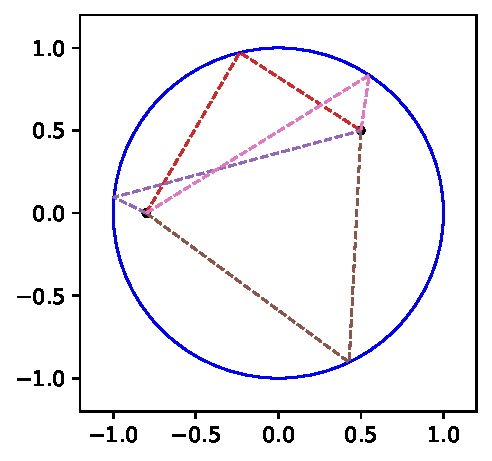
\includegraphics{./ADOneDimManually_files/figure-pdf/fig-billardproblemsolution-output-1.pdf}

}

\caption{\label{fig-billardproblemsolution}Lösung des Billardproblems.}

\end{figure}

\end{tcolorbox}

\hypertarget{sec-SadImplementationOperatorOverloading}{%
\section{Implementation der SAD mit Operator
Overloading}\label{sec-SadImplementationOperatorOverloading}}

Nach dem letzten Abschnitt könnte man einwenden, dass wir die
Ableitungen der Funktionen ja doch von Hand berechnet haben, denn wir
haben jede Programmzeile, in der eine Variable \texttt{v} berechnet
wird, um eine weitere Zeile ergänzt, in der wir \texttt{vdot} nach den
bekannten Ableitungsregeln berechnet haben. Dieser Einwand ist auch
berechtigt - oder wie es Henrard ausdrückt:

\begin{quote}
``The bad news is that it {[}calculating the derivatives{]} has to be
done; it will not appear magically. It is not only a figure of speech
that `something has to be done' but that to have it working everything
has to be done''. (Henrard 2017, 17)
\end{quote}

Die gute Nachricht ist, dass wir diesen Prozess weiter automatisieren
können. Wir kennen die Ableitungsregeln für die elementaren Operationen
(\texttt{+,-,*,/}), sowie für die Grundfunktionen. In diesem Abschnitt
werden wir eine Klasse \texttt{FloatSad} schreiben, deren Instanzen
Funktionswerte und Werte der Ableitung speichern. Da solche Werte in der
Regel vom Typ \texttt{float} sind und wir die Standard-AD
implementieren, nennen wir die Klasse \texttt{FloatSad}. Die Arbeit
besteht dann darin, die Ableitungsregeln richtig in den Operatoren
dieser Klasse zu kodieren. Da Python \emph{Operator Overloading} kennt,
werden wir dann nach getaner Arbeit die Ableitungen wirklich ohne
zusätzlichen Programmieraufwand erhalten.

Der Grundstein für unsere Klasse wurde bereits im 19. Jahrhundert
gelegt, wie die folgende Infobox zeigt:

\begin{tcolorbox}[enhanced jigsaw, title=\textcolor{quarto-callout-note-color}{\faInfo}\hspace{0.5em}{Hintergrund: Duale Zahlen}, colbacktitle=quarto-callout-note-color!10!white, bottomrule=.15mm, titlerule=0mm, colback=white, breakable, colframe=quarto-callout-note-color-frame, bottomtitle=1mm, toptitle=1mm, leftrule=.75mm, arc=.35mm, left=2mm, rightrule=.15mm, toprule=.15mm, opacitybacktitle=0.6, opacityback=0, coltitle=black]
Duale Zahlen wurden 1873 durch William Clifford eingeführt und sind
ähnlich definiert, wie komplexe Zahlen. Zur Erinnerung: Eine komplexe
Zahl ist eine Zahl der Form \(a + bi\),wobei \(a,b \in \mathbb{R}\) sind
und \(i\) die Eigenschaft \(i^2 = -1\) hat. Eine duale Zahl ist eine
Zahl der Form \(a + a'\epsilon\), wobei wieder \(a,a' \in \mathbb{R}\)
gilt, aber \(\epsilon\) die Eigenschaft \(\epsilon^2 = 0\) hat. Nun kann
man nach dem Permanenzprinzip die folgenden Operationen für duale Zahlen
definieren: \[
\begin{alignat}{3}
    &\textrm{Addition:} && (a+a'\epsilon) + (b+b'\epsilon) &&= (a+b) + (a'+b')\epsilon \\ \\
    &\textrm{Subtraktion:} && (a+a'\epsilon) - (b+b'\epsilon) &&= (a-b) + (a'-b')\epsilon \\ \\
    &\textrm{Multiplikation:}\quad && (a+a'\epsilon) \cdot (b+b'\epsilon) &&= ab + a'b\epsilon + ab'\epsilon + a'b'\epsilon^2 \\
    & && &&= ab + (a'b + ab')\epsilon \\ \\
    &\textrm{Division:} && (\textrm{für }b\ne 0) \quad \frac{a+a'\epsilon}{b+b'\epsilon} &&= \frac{(a+a'\epsilon)(b-b'\epsilon)}{(b+b'\epsilon)(b-b'\epsilon)} \\
    & && &&= \frac{ab+a'b\epsilon-ab'\epsilon-a'b'\epsilon^2}{b^2 - (b')^2\epsilon^2} \\ 
    & && &&= \frac{ab + (a'b-ab')\epsilon}{b^2} \\ 
    & && &&= \frac{a}{b} + \frac{a'b - ab'}{b^2} \epsilon
\end{alignat}
\] Wir sehen, dass der reelle Teil den Wert der Operation und der duale
Teil den Wert der zugehörigen Ableitung enthält. Dies gilt auch für
Potenzen, wie man unter Anwendung des binomischen Satzes sieht: \[
\begin{align}
    (a+a'\epsilon)^n &= \sum_{k=0}^n \binom n k a^{n-k} (a'\epsilon)^k  \\
    &= a^n + n \cdot a^{n-1} \cdot a'\epsilon + (\textrm{Terme mit }\epsilon^2) \\ 
    &= a^n + n \cdot a^{n-1} \cdot a' \epsilon
\end{align}
\] Im dualen Teil erkennen wir die Kettenregel
\((a^n)' = n\cdot a^{n-1}\cdot a'\). Damit können wir duale Zahlen auch
in Polynome \(p(x) = p_0 + p_1 x + p_2 x^2 + \ldots + p_n x^n\)
einsetzen. Wir erhalten dann \[
\begin{align}
    p(a+a'\epsilon) &= p_0 + p_1 (a+a'\epsilon) + p_2 (a+a'\epsilon)^2 + \ldots + p_n (a+a'\epsilon)^n \\ 
    &= p_0 + p_1 a + p_1 a'\epsilon + p_2 a^2 + p_2 \cdot 2a a' \epsilon + ... + p_n a^n + p_n \cdot n a^{n-1} a' \epsilon \\ 
    &= p_0 + p_1 a + p_2 a^2 + \ldots p_n a^n + (p_1 + p_2 \cdot 2a + \ldots + p_n \cdot n a^{n-1}) \cdot a' \epsilon \\
    &= p(a) + p'(a) \cdot a'\epsilon
\end{align}
\] Dieses Resultat lässt sich auf allgemeine Funktionen \(f\)
verallgemeinern (für den Beweis entwickelt man \(f\) in eine Taylorreihe
und macht die gleichen Überlegungen wie für ein Polynom): \[
f(a+a'\epsilon) = f(a) + f'(a)\cdot a'\epsilon
\]

(\href{https://en.wikipedia.org/wiki/Dual_number}{Wikipedia: Dual
number} und Slater (2022))
\end{tcolorbox}

\hypertarget{sec-FoatSadClassDescription}{%
\subsection{\texorpdfstring{Die Klasse
\texttt{FloatSad}}{Die Klasse FloatSad}}\label{sec-FoatSadClassDescription}}

Beginnen wir nun mit der Implementation unserer Klasse
\texttt{FloatSad}. Analog zu den dualen Zahlen enthält jedes
\texttt{FloatSad}-Objekt zwei Attribute. Das Attribut \texttt{value}
speichert den Funktionswert und das Attribut \texttt{derivative}
speichert den Wert der Ableitung. Im Konstruktor der Klasse setzen wir
für \texttt{derivative} den Standardwert \texttt{1}. Damit können wir
eine gewöhnliche \texttt{Float}-Zahl korrekt in ein \texttt{FloatSad}
umwandeln. Dies wird im \texttt{main} Programm demonstriert.

\begin{Shaded}
\begin{Highlighting}[]
\ImportTok{import}\NormalTok{ math}

\KeywordTok{class}\NormalTok{ FloatSad:}

    \KeywordTok{def} \FunctionTok{\_\_init\_\_}\NormalTok{(}\VariableTok{self}\NormalTok{, value, derivative }\OperatorTok{=} \FloatTok{1.0}\NormalTok{):}
        \VariableTok{self}\NormalTok{.value }\OperatorTok{=} \BuiltInTok{float}\NormalTok{(value)}
        \VariableTok{self}\NormalTok{.derivative }\OperatorTok{=}\NormalTok{ derivative}


\ControlFlowTok{if} \VariableTok{\_\_name\_\_} \OperatorTok{==} \StringTok{\textquotesingle{}\_\_main\_\_\textquotesingle{}}\NormalTok{:}

    \KeywordTok{def}\NormalTok{ f(x):}
\NormalTok{        v0 }\OperatorTok{=}\NormalTok{ FloatSad(x)}
\NormalTok{        y }\OperatorTok{=}\NormalTok{ v0}
        \ControlFlowTok{return}\NormalTok{ y}

\NormalTok{    x0 }\OperatorTok{=} \DecValTok{2}
\NormalTok{    resultat }\OperatorTok{=}\NormalTok{ f(x0)}
    \BuiltInTok{print}\NormalTok{(}\StringTok{"Funktionswert:"}\NormalTok{, resultat.value)}
    \BuiltInTok{print}\NormalTok{(}\StringTok{"Ableitung:"}\NormalTok{, resultat.derivative)}
\end{Highlighting}
\end{Shaded}

\begin{verbatim}
Funktionswert: 2.0
Ableitung: 1.0
\end{verbatim}

In der Funktion \texttt{f} haben wir nun unsere Konvention, dass
\texttt{v0\ =\ x} sein soll, dazu verwendet, den Zahlenwert \texttt{x}
in ein \texttt{FloatSad}-Objekt umzuwandeln. Die Konvention
\texttt{v0dot\ =\ 1} ist im Konstruktor kodiert. Von nun an machen wir
also die folgende Konvention:

\begin{tcolorbox}[enhanced jigsaw, title=\textcolor{quarto-callout-important-color}{\faExclamation}\hspace{0.5em}{Konvention}, colbacktitle=quarto-callout-important-color!10!white, bottomrule=.15mm, titlerule=0mm, colback=white, breakable, colframe=quarto-callout-important-color-frame, bottomtitle=1mm, toptitle=1mm, leftrule=.75mm, arc=.35mm, left=2mm, rightrule=.15mm, toprule=.15mm, opacitybacktitle=0.6, opacityback=0, coltitle=black]
Eine Funktion berechnet aus einem Argument \texttt{x} vom Typ
\texttt{float} oder \texttt{int} einen Rückgabewert \texttt{y} vom Typ
\texttt{FloatSad} über eine Reihe von Hilfsvariablen \texttt{v}, die
alle vom Typ \texttt{FloatSad} sind. Insbesondere setzen wir am Anfang
immer \texttt{v0\ =\ FloatSad(x)}.
\end{tcolorbox}

Das obige Programm berechnet also den Funktionswert und den Wert der
Ableitung von \(f(x) = x\) an der Stelle \(x_0 = 2\).

Um die Ausgabe etwas einfacher zu gestalten implementieren wir als
nächstes die \texttt{print} Methode für unsere Klasse. Wir geben ein
\texttt{FloatSad}-Objekt einfach in der Form
\texttt{\textless{}\ value\ ;\ derivative\ \textgreater{}} aus.

\begin{Shaded}
\begin{Highlighting}[]
\KeywordTok{def} \FunctionTok{\_\_repr\_\_}\NormalTok{(}\VariableTok{self}\NormalTok{):}
        \ControlFlowTok{return} \StringTok{"\textless{} "} \OperatorTok{+} \BuiltInTok{str}\NormalTok{(}\VariableTok{self}\NormalTok{.value) }\OperatorTok{+} \StringTok{" ; "} \OperatorTok{+} \BuiltInTok{str}\NormalTok{(}\VariableTok{self}\NormalTok{.derivative) }\OperatorTok{+} \StringTok{" \textgreater{}"}
\end{Highlighting}
\end{Shaded}

Da wir nun die Funktion \(f(x) = x\) programmieren können, wollen wir
als nächstes auch die Funktion \(f(x) = -x\) programmieren können. Wir
müssen unsere \texttt{FloatSad}-Objekte also mit Vorzeichen versehen.

\hypertarget{vorzeichen}{%
\subsection{Vorzeichen}\label{vorzeichen}}

Natürlich wollen wir nicht nur das negative Vorzeichen, sondern auch das
positive Vorzeichen implementieren, damit wir in unseren Programmen z.B.
\texttt{v1\ =\ +v0} oder \texttt{v2\ =\ -v0} schreiben können. Beim
positiven Vorzeichen müssen wir nichts machen, wir geben also ein
\texttt{FloatSad}-Objekt mit den gleichen Attributen zurück. Beim
negativen Vorzeichen ändern beide Attribute ihr Vorzeichen.

\begin{Shaded}
\begin{Highlighting}[]
\KeywordTok{def} \FunctionTok{\_\_pos\_\_}\NormalTok{(}\VariableTok{self}\NormalTok{):}
        \ControlFlowTok{return}\NormalTok{ FloatSad(}\VariableTok{self}\NormalTok{.value, }\VariableTok{self}\NormalTok{.derivative)}
    
\KeywordTok{def} \FunctionTok{\_\_neg\_\_}\NormalTok{(}\VariableTok{self}\NormalTok{):}
\NormalTok{    newValue }\OperatorTok{=} \OperatorTok{{-}}\VariableTok{self}\NormalTok{.value}
\NormalTok{    newDerivative }\OperatorTok{=} \OperatorTok{{-}}\VariableTok{self}\NormalTok{.derivative}
    \ControlFlowTok{return}\NormalTok{ FloatSad(newValue, newDerivative)}
\end{Highlighting}
\end{Shaded}

Nun gehen wir daran, die Grundoperationen für \texttt{FloatSad}-Objekte
zu implementieren.

\hypertarget{die-operatoren-und--}{%
\subsection{\texorpdfstring{Die Operatoren \texttt{+} und
\texttt{-}}{Die Operatoren + und -}}\label{die-operatoren-und--}}

Wir möchten in unseren Programmen Anweisungen wie
\texttt{v2\ =\ v0\ +\ v1} verwenden können. Gemäss der Summenregel
können wir dazu einfach die Funktionswerte und auch die Werte der
Ableitungen addieren.

\begin{Shaded}
\begin{Highlighting}[]
\KeywordTok{def} \FunctionTok{\_\_add\_\_}\NormalTok{(}\VariableTok{self}\NormalTok{, other):}
\NormalTok{        newValue }\OperatorTok{=} \VariableTok{self}\NormalTok{.value }\OperatorTok{+}\NormalTok{ other.value}
\NormalTok{        newDerivative }\OperatorTok{=} \VariableTok{self}\NormalTok{.derivative }\OperatorTok{+}\NormalTok{ other.derivative}
        \ControlFlowTok{return}\NormalTok{ FloatSad(newValue, newDerivative)}
\end{Highlighting}
\end{Shaded}

Nun können wir zwei \texttt{FloatSad}-Objekte miteinander addieren.
Manchmal möchten wir aber auch ein \texttt{float}- oder
\texttt{int}-Wert zu einem \texttt{FloatSad}-Objekt addieren, z.B.
\texttt{v1\ =\ v0\ +\ 2}. Dazu machen wir eine Typabfrage und passen den
Wert der Ableitung entsprechend der Konstantenregel an:

\begin{Shaded}
\begin{Highlighting}[]
\KeywordTok{def} \FunctionTok{\_\_add\_\_}\NormalTok{(}\VariableTok{self}\NormalTok{, other):}
    \ControlFlowTok{if} \BuiltInTok{type}\NormalTok{(other) }\KeywordTok{in}\NormalTok{ (}\BuiltInTok{float}\NormalTok{, }\BuiltInTok{int}\NormalTok{):}
\NormalTok{        newValue }\OperatorTok{=} \VariableTok{self}\NormalTok{.value }\OperatorTok{+}\NormalTok{ other}
\NormalTok{        newDerivative }\OperatorTok{=} \VariableTok{self}\NormalTok{.derivative }\OperatorTok{+} \FloatTok{0.0}
    \ControlFlowTok{else}\NormalTok{:}
\NormalTok{        newValue }\OperatorTok{=} \VariableTok{self}\NormalTok{.value }\OperatorTok{+}\NormalTok{ other.value}
\NormalTok{        newDerivative }\OperatorTok{=} \VariableTok{self}\NormalTok{.derivative }\OperatorTok{+}\NormalTok{ other.derivative}
    \ControlFlowTok{return}\NormalTok{ FloatSad(newValue, newDerivative)}
\end{Highlighting}
\end{Shaded}

Jetzt funktioniert zwar die Anweisung \texttt{v1\ =\ v0\ +\ 2}, aber die
Anweisung \texttt{v1\ =\ 2\ +\ v0} erzeugt immer noch eine
Fehlermeldung. Um dieses Problem zu beheben, müssen wir als nächstes den
\emph{reverse-add}-Operator implementieren.

\begin{Shaded}
\begin{Highlighting}[]
\KeywordTok{def} \FunctionTok{\_\_radd\_\_}\NormalTok{(}\VariableTok{self}\NormalTok{, other):}
    \ControlFlowTok{if} \BuiltInTok{type}\NormalTok{(other) }\KeywordTok{in}\NormalTok{ (}\BuiltInTok{float}\NormalTok{, }\BuiltInTok{int}\NormalTok{):}
\NormalTok{        newValue }\OperatorTok{=}\NormalTok{ other }\OperatorTok{+} \VariableTok{self}\NormalTok{.value}
\NormalTok{        newDerivative }\OperatorTok{=} \FloatTok{0.0} \OperatorTok{+} \VariableTok{self}\NormalTok{.derivative}
    \ControlFlowTok{else}\NormalTok{:}
\NormalTok{        newValue }\OperatorTok{=}\NormalTok{ other.value }\OperatorTok{+} \VariableTok{self}\NormalTok{.value}
\NormalTok{        newDerivative }\OperatorTok{=}\NormalTok{ other.derivative }\OperatorTok{+} \VariableTok{self}\NormalTok{.derivative}
    \ControlFlowTok{return}\NormalTok{ FloatSad(newValue, newDerivative)}
\end{Highlighting}
\end{Shaded}

Hier ist die bisher implementierte Klasse zusammen mit einem kleinen
Testprogramm.

\begin{Shaded}
\begin{Highlighting}[]
\ImportTok{import}\NormalTok{ math}

\KeywordTok{class}\NormalTok{ FloatSad:}

    \KeywordTok{def} \FunctionTok{\_\_init\_\_}\NormalTok{(}\VariableTok{self}\NormalTok{, value, derivative }\OperatorTok{=} \FloatTok{1.0}\NormalTok{):}
        \VariableTok{self}\NormalTok{.value }\OperatorTok{=} \BuiltInTok{float}\NormalTok{(value)}
        \VariableTok{self}\NormalTok{.derivative }\OperatorTok{=}\NormalTok{ derivative}

    \KeywordTok{def} \FunctionTok{\_\_repr\_\_}\NormalTok{(}\VariableTok{self}\NormalTok{):}
        \ControlFlowTok{return} \StringTok{"\textless{} "} \OperatorTok{+} \BuiltInTok{str}\NormalTok{(}\VariableTok{self}\NormalTok{.value) }\OperatorTok{+} \StringTok{" ; "} \OperatorTok{+} \BuiltInTok{str}\NormalTok{(}\VariableTok{self}\NormalTok{.derivative) }\OperatorTok{+} \StringTok{" \textgreater{}"}


    \CommentTok{\# unäre Operatoren}

    \KeywordTok{def} \FunctionTok{\_\_pos\_\_}\NormalTok{(}\VariableTok{self}\NormalTok{):}
        \ControlFlowTok{return}\NormalTok{ FloatSad(}\VariableTok{self}\NormalTok{.value, }\VariableTok{self}\NormalTok{.derivative)}
    
    \KeywordTok{def} \FunctionTok{\_\_neg\_\_}\NormalTok{(}\VariableTok{self}\NormalTok{):}
\NormalTok{        newValue }\OperatorTok{=} \OperatorTok{{-}}\VariableTok{self}\NormalTok{.value}
\NormalTok{        newDerivative }\OperatorTok{=} \OperatorTok{{-}}\VariableTok{self}\NormalTok{.derivative}
        \ControlFlowTok{return}\NormalTok{ FloatSad(newValue, newDerivative)}
    

    \CommentTok{\# binäre Operatoren}

    \KeywordTok{def} \FunctionTok{\_\_add\_\_}\NormalTok{(}\VariableTok{self}\NormalTok{, other):}
        \ControlFlowTok{if} \BuiltInTok{type}\NormalTok{(other) }\KeywordTok{in}\NormalTok{ (}\BuiltInTok{float}\NormalTok{, }\BuiltInTok{int}\NormalTok{):}
\NormalTok{            newValue }\OperatorTok{=} \VariableTok{self}\NormalTok{.value }\OperatorTok{+}\NormalTok{ other}
\NormalTok{            newDerivative }\OperatorTok{=} \VariableTok{self}\NormalTok{.derivative }\OperatorTok{+} \FloatTok{0.0}
        \ControlFlowTok{else}\NormalTok{:}
\NormalTok{            newValue }\OperatorTok{=} \VariableTok{self}\NormalTok{.value }\OperatorTok{+}\NormalTok{ other.value}
\NormalTok{            newDerivative }\OperatorTok{=} \VariableTok{self}\NormalTok{.derivative }\OperatorTok{+}\NormalTok{ other.derivative}
        \ControlFlowTok{return}\NormalTok{ FloatSad(newValue, newDerivative)}

    \KeywordTok{def} \FunctionTok{\_\_radd\_\_}\NormalTok{(}\VariableTok{self}\NormalTok{, other):}
        \ControlFlowTok{if} \BuiltInTok{type}\NormalTok{(other) }\KeywordTok{in}\NormalTok{ (}\BuiltInTok{float}\NormalTok{, }\BuiltInTok{int}\NormalTok{):}
\NormalTok{            newValue }\OperatorTok{=}\NormalTok{ other }\OperatorTok{+} \VariableTok{self}\NormalTok{.value}
\NormalTok{            newDerivative }\OperatorTok{=} \FloatTok{0.0} \OperatorTok{+} \VariableTok{self}\NormalTok{.derivative}
        \ControlFlowTok{else}\NormalTok{:}
\NormalTok{            newValue }\OperatorTok{=}\NormalTok{ other.value }\OperatorTok{+} \VariableTok{self}\NormalTok{.value}
\NormalTok{            newDerivative }\OperatorTok{=}\NormalTok{ other.derivative }\OperatorTok{+} \VariableTok{self}\NormalTok{.derivative}
        \ControlFlowTok{return}\NormalTok{ FloatSad(newValue, newDerivative)}
    


\ControlFlowTok{if} \VariableTok{\_\_name\_\_} \OperatorTok{==} \StringTok{\textquotesingle{}\_\_main\_\_\textquotesingle{}}\NormalTok{:}

    \KeywordTok{def}\NormalTok{ f(x):}
\NormalTok{        v0 }\OperatorTok{=}\NormalTok{ FloatSad(x)}
\NormalTok{        v1 }\OperatorTok{=} \OperatorTok{{-}}\NormalTok{v0 }
\NormalTok{        v2 }\OperatorTok{=} \DecValTok{3} \OperatorTok{+}\NormalTok{ v1}
\NormalTok{        v3 }\OperatorTok{=}\NormalTok{ v2 }\OperatorTok{+}\NormalTok{ v1}
\NormalTok{        y  }\OperatorTok{=} \OperatorTok{+}\NormalTok{v3}
        \ControlFlowTok{return}\NormalTok{ y}

\NormalTok{    resultat }\OperatorTok{=}\NormalTok{ f(}\DecValTok{2}\NormalTok{)}
    \BuiltInTok{print}\NormalTok{(resultat)}
\end{Highlighting}
\end{Shaded}

\begin{verbatim}
< -1.0 ; -2.0 >
\end{verbatim}

\leavevmode\vadjust pre{\hypertarget{exr-verifyFirstSADderivative}{}}%
\begin{exercise}[Korrektheit
überprüfen]\label{exr-verifyFirstSADderivative}

Welche Funktion berechnet \texttt{f} im \texttt{main} Programm? Stimmt
die Ausgabe?

\end{exercise}

\begin{tcolorbox}[enhanced jigsaw, title=\textcolor{quarto-callout-tip-color}{\faLightbulb}\hspace{0.5em}{Lösung}, colbacktitle=quarto-callout-tip-color!10!white, bottomrule=.15mm, titlerule=0mm, colback=white, breakable, colframe=quarto-callout-tip-color-frame, bottomtitle=1mm, toptitle=1mm, leftrule=.75mm, arc=.35mm, left=2mm, rightrule=.15mm, toprule=.15mm, opacitybacktitle=0.6, opacityback=0, coltitle=black]
Es handelt sich um die Funktion \(f(x) = 3 - 2x\). Die Ausgabe
\(f(2) = -1, f'(2) = -2\) ist also korrekt.
\end{tcolorbox}

Für die nächste Übung musst du das obige Programm kopieren und in einer
Datei mit dem Namen \texttt{floatsad.py} abspeichern. Speichere die
Datei im gleichen Ordner wie die anderen Dateien.

\leavevmode\vadjust pre{\hypertarget{exr-ImplementSub}{}}%
\begin{exercise}[Den Operator \texttt{-}
implementieren]\label{exr-ImplementSub}

Implementiere auf die gleiche Weise den \texttt{-}-Operator. Die
Methoden lauten \texttt{\_\_sub\_\_(self,\ other)} bzw.
\texttt{\_\_rsub\_\_(self,\ other)}. Schreibe auch eine Testfunktion
\texttt{f}, welche die neuen Operatoren verwendet.

\end{exercise}

\begin{tcolorbox}[enhanced jigsaw, title=\textcolor{quarto-callout-tip-color}{\faLightbulb}\hspace{0.5em}{Lösung}, colbacktitle=quarto-callout-tip-color!10!white, bottomrule=.15mm, titlerule=0mm, colback=white, breakable, colframe=quarto-callout-tip-color-frame, bottomtitle=1mm, toptitle=1mm, leftrule=.75mm, arc=.35mm, left=2mm, rightrule=.15mm, toprule=.15mm, opacitybacktitle=0.6, opacityback=0, coltitle=black]

\begin{Shaded}
\begin{Highlighting}[]
\KeywordTok{def} \FunctionTok{\_\_sub\_\_}\NormalTok{(}\VariableTok{self}\NormalTok{, other):}
    \ControlFlowTok{if} \BuiltInTok{type}\NormalTok{(other) }\KeywordTok{in}\NormalTok{ (}\BuiltInTok{float}\NormalTok{, }\BuiltInTok{int}\NormalTok{):}
\NormalTok{        newValue }\OperatorTok{=} \VariableTok{self}\NormalTok{.value }\OperatorTok{{-}}\NormalTok{ other}
\NormalTok{        newDerivative }\OperatorTok{=} \VariableTok{self}\NormalTok{.derivative }\OperatorTok{{-}} \FloatTok{0.0}
    \ControlFlowTok{else}\NormalTok{:}
\NormalTok{        newValue }\OperatorTok{=} \VariableTok{self}\NormalTok{.value }\OperatorTok{{-}}\NormalTok{ other.value}
\NormalTok{        newDerivative }\OperatorTok{=} \VariableTok{self}\NormalTok{.derivative }\OperatorTok{{-}}\NormalTok{ other.derivative}
    \ControlFlowTok{return}\NormalTok{ FloatSad(newValue, newDerivative)}

\KeywordTok{def} \FunctionTok{\_\_rsub\_\_}\NormalTok{(}\VariableTok{self}\NormalTok{, other):}
    \ControlFlowTok{if} \BuiltInTok{type}\NormalTok{(other) }\KeywordTok{in}\NormalTok{ (}\BuiltInTok{float}\NormalTok{, }\BuiltInTok{int}\NormalTok{):}
\NormalTok{        newValue }\OperatorTok{=}\NormalTok{ other }\OperatorTok{{-}} \VariableTok{self}\NormalTok{.value}
\NormalTok{        newDerivative }\OperatorTok{=} \FloatTok{0.0} \OperatorTok{{-}} \VariableTok{self}\NormalTok{.derivative}
    \ControlFlowTok{else}\NormalTok{:}
\NormalTok{        newValue }\OperatorTok{=}\NormalTok{ other.value }\OperatorTok{{-}} \VariableTok{self}\NormalTok{.value}
\NormalTok{        newDerivative }\OperatorTok{=}\NormalTok{ other.derivative }\OperatorTok{{-}} \VariableTok{self}\NormalTok{.derivative}
    \ControlFlowTok{return}\NormalTok{ FloatSad(newValue, newDerivative)}
\end{Highlighting}
\end{Shaded}

\end{tcolorbox}

\hypertarget{die-operatoren-und}{%
\subsection{\texorpdfstring{Die Operatoren \texttt{*} und
\texttt{/}}{Die Operatoren * und /}}\label{die-operatoren-und}}

Als nächstes wollen wir die Multiplikation implementieren, um
Anweisungen der Form \texttt{v2\ =\ v0\ *\ v1} ausführen zu können. Dazu
müssen wir die Produktregel verwenden. Wie bei der Addition und der
Subtraktion soll unser \texttt{*}-Operator aber auch Anweisungen der
Form \texttt{v1\ =\ v0\ *\ 2} oder \texttt{v1\ =\ -3\ *\ v0} richtig
auswerten, bei denen die Faktorregel angewendet wird. Dazu ist wieder
eine Typabfrage nötig.

\leavevmode\vadjust pre{\hypertarget{exr-ImplementMul}{}}%
\begin{exercise}[Den Operator \texttt{*}
implementieren]\label{exr-ImplementMul}

Ergänze die Datei \texttt{floatsad.py} mit den Methoden
\texttt{\_\_mul\_\_(self,\ other)} und
\texttt{\_\_rmul\_\_(self,\ other)}. Überlege dir verschiedene Testfälle
und überzeuge dich von der Korrektheit deines Programms.

\end{exercise}

\begin{tcolorbox}[enhanced jigsaw, title=\textcolor{quarto-callout-tip-color}{\faLightbulb}\hspace{0.5em}{Lösung}, colbacktitle=quarto-callout-tip-color!10!white, bottomrule=.15mm, titlerule=0mm, colback=white, breakable, colframe=quarto-callout-tip-color-frame, bottomtitle=1mm, toptitle=1mm, leftrule=.75mm, arc=.35mm, left=2mm, rightrule=.15mm, toprule=.15mm, opacitybacktitle=0.6, opacityback=0, coltitle=black]

\begin{Shaded}
\begin{Highlighting}[]
\KeywordTok{def} \FunctionTok{\_\_mul\_\_}\NormalTok{(}\VariableTok{self}\NormalTok{, other):}
    \ControlFlowTok{if} \BuiltInTok{type}\NormalTok{(other) }\KeywordTok{in}\NormalTok{ (}\BuiltInTok{float}\NormalTok{, }\BuiltInTok{int}\NormalTok{):}
\NormalTok{        newValue }\OperatorTok{=} \VariableTok{self}\NormalTok{.value }\OperatorTok{*}\NormalTok{ other}
\NormalTok{        newDerivative }\OperatorTok{=} \VariableTok{self}\NormalTok{.derivative }\OperatorTok{*}\NormalTok{ other}
    \ControlFlowTok{else}\NormalTok{:}
\NormalTok{        newValue }\OperatorTok{=} \VariableTok{self}\NormalTok{.value }\OperatorTok{*}\NormalTok{ other.value}
\NormalTok{        newDerivative }\OperatorTok{=} \VariableTok{self}\NormalTok{.derivative }\OperatorTok{*}\NormalTok{ other.value }\OperatorTok{+} \VariableTok{self}\NormalTok{.value }\OperatorTok{*}\NormalTok{ other.derivative}
    \ControlFlowTok{return}\NormalTok{ FloatSad(newValue, newDerivative)}

\KeywordTok{def} \FunctionTok{\_\_rmul\_\_}\NormalTok{(}\VariableTok{self}\NormalTok{, other):}
    \ControlFlowTok{if} \BuiltInTok{type}\NormalTok{(other) }\KeywordTok{in}\NormalTok{ (}\BuiltInTok{float}\NormalTok{, }\BuiltInTok{int}\NormalTok{):}
\NormalTok{        newValue }\OperatorTok{=}\NormalTok{ other }\OperatorTok{*} \VariableTok{self}\NormalTok{.value}
\NormalTok{        newDerivative }\OperatorTok{=}\NormalTok{ other }\OperatorTok{*} \VariableTok{self}\NormalTok{.derivative}
    \ControlFlowTok{else}\NormalTok{:}
\NormalTok{        newValue }\OperatorTok{=}\NormalTok{ other.value }\OperatorTok{*} \VariableTok{self}\NormalTok{.value}
\NormalTok{        newDerivative }\OperatorTok{=}\NormalTok{  other.derivative }\OperatorTok{*} \VariableTok{self}\NormalTok{.value }\OperatorTok{+}\NormalTok{ other.value }\OperatorTok{*} \VariableTok{self}\NormalTok{.derivative}
    \ControlFlowTok{return}\NormalTok{ FloatSad(newValue, newDerivative)}
\end{Highlighting}
\end{Shaded}

\end{tcolorbox}

Es fehlt noch der Divisionsoperator, damit wir Anweisungen wie
\texttt{v2\ =\ v1\ /\ v0} verwenden können. Da wir es bei
differenzierbaren Funktionen immer mit \texttt{float}- bzw.
\texttt{FloatSad}-Objekten zu tun haben, implementieren wir nur den
\texttt{/}-Operator, also die Funktion
\texttt{\_\_truediv\_\_(self,\ other)} und nicht den
\texttt{//}-Operator. Wir wollen aber wieder die Fallunterscheidung nach
den Typen machen, so dass auch Anweisungen wie \texttt{v1\ =\ v0\ /\ 4}
verwendet werden können. Dabei benötigen wir nur die Faktorregel und
nicht die Quotientenregel. Um schliesslich auch noch
\texttt{v1\ =\ -4\ /\ v0} zu ermöglichen, muss noch
\texttt{\_\_rtruediv\_\_(self,\ other)} implementiert werden. Bei
letzterem darf nicht vergessen werden, dass auch die Kettenregel benutzt
werden muss, denn
\(\frac{dv_1}{dx} = \frac{dv_1}{dv_0}\cdot \frac{dv_0}{dx} = \frac{4}{v_0^2}\cdot v_0'\).
Quadrate kann man mit \texttt{math.pow(value,\ 2)} berechnen. Bei der
Implementierung müssen wir uns übrigens nicht um Fehlerbehandlungen, wie
das Abfangen einer Division durch Null, kümmern, weil diese bereits im
\texttt{/}-Operator, den wir verwenden, implementiert sind.

\leavevmode\vadjust pre{\hypertarget{exr-ImplementTrueDiv}{}}%
\begin{exercise}[Den Operator \texttt{/}
implementieren]\label{exr-ImplementTrueDiv}

Ergänze die Datei \texttt{floatsad.py} mit den Methoden
\texttt{\_\_truediv\_\_(self,\ other)} und
\texttt{\_\_rtruediv\_\_(self,\ other)}. Überlege dir auch wieder
verschiedene Testfälle und überzeuge dich von der Korrektheit deines
Programms.

\end{exercise}

\begin{tcolorbox}[enhanced jigsaw, title=\textcolor{quarto-callout-tip-color}{\faLightbulb}\hspace{0.5em}{Lösung}, colbacktitle=quarto-callout-tip-color!10!white, bottomrule=.15mm, titlerule=0mm, colback=white, breakable, colframe=quarto-callout-tip-color-frame, bottomtitle=1mm, toptitle=1mm, leftrule=.75mm, arc=.35mm, left=2mm, rightrule=.15mm, toprule=.15mm, opacitybacktitle=0.6, opacityback=0, coltitle=black]

\begin{Shaded}
\begin{Highlighting}[]
\KeywordTok{def} \FunctionTok{\_\_truediv\_\_}\NormalTok{(}\VariableTok{self}\NormalTok{, other):}
    \ControlFlowTok{if} \BuiltInTok{type}\NormalTok{(other) }\KeywordTok{in}\NormalTok{ (}\BuiltInTok{float}\NormalTok{, }\BuiltInTok{int}\NormalTok{):}
\NormalTok{        newValue }\OperatorTok{=} \VariableTok{self}\NormalTok{.value }\OperatorTok{/}\NormalTok{ other}
\NormalTok{        newDerivative }\OperatorTok{=} \VariableTok{self}\NormalTok{.derivative }\OperatorTok{/}\NormalTok{ other}
    \ControlFlowTok{else}\NormalTok{:}
\NormalTok{        newValue }\OperatorTok{=} \VariableTok{self}\NormalTok{.value }\OperatorTok{/}\NormalTok{ other.value}
\NormalTok{        newDerivative }\OperatorTok{=}\NormalTok{ (}\VariableTok{self}\NormalTok{.derivative }\OperatorTok{*}\NormalTok{ other.value }\OperatorTok{{-}} \VariableTok{self}\NormalTok{.value }\OperatorTok{*}\NormalTok{ other.derivative) }\OperatorTok{/}\NormalTok{ math.}\BuiltInTok{pow}\NormalTok{(other.value, }\DecValTok{2}\NormalTok{)}
    \ControlFlowTok{return}\NormalTok{ FloatSad(newValue, newDerivative)}

\KeywordTok{def} \FunctionTok{\_\_rtruediv\_\_}\NormalTok{(}\VariableTok{self}\NormalTok{, other):}
    \ControlFlowTok{if} \BuiltInTok{type}\NormalTok{(other) }\KeywordTok{in}\NormalTok{ (}\BuiltInTok{float}\NormalTok{, }\BuiltInTok{int}\NormalTok{):}
\NormalTok{        newValue }\OperatorTok{=}\NormalTok{ other }\OperatorTok{/} \VariableTok{self}\NormalTok{.value}
\NormalTok{        newDerivative }\OperatorTok{=} \OperatorTok{{-}}\NormalTok{ other }\OperatorTok{/}\NormalTok{ math.}\BuiltInTok{pow}\NormalTok{(}\VariableTok{self}\NormalTok{.value, }\DecValTok{2}\NormalTok{) }\OperatorTok{*} \VariableTok{self}\NormalTok{.derivative}
    \ControlFlowTok{else}\NormalTok{:}
\NormalTok{        newValue }\OperatorTok{=}\NormalTok{ other.value }\OperatorTok{/} \VariableTok{self}\NormalTok{.value}
\NormalTok{        newDerivative }\OperatorTok{=}\NormalTok{ (other.derivative }\OperatorTok{*} \VariableTok{self}\NormalTok{.value }\OperatorTok{{-}}\NormalTok{ other.value }\OperatorTok{*} \VariableTok{self}\NormalTok{.derivative) }\OperatorTok{/}\NormalTok{ math.}\BuiltInTok{pow}\NormalTok{(}\VariableTok{self}\NormalTok{.value, }\DecValTok{2}\NormalTok{) }\OperatorTok{*} \VariableTok{self}\NormalTok{.derivative}
    \ControlFlowTok{return}\NormalTok{ FloatSad(newValue, newDerivative)}
\end{Highlighting}
\end{Shaded}

\end{tcolorbox}

\hypertarget{der-operator}{%
\subsection{\texorpdfstring{Der Operator
\texttt{**}}{Der Operator **}}\label{der-operator}}

Interessant ist nun die Implementation des Potenzoperators. Hier sind
mehrere Fallunterscheidungen nötig.

Betrachten wir zuerst den Fall, \texttt{type(other)\ in\ (float,\ int)},
d.h. wir haben einen Ausdruck der Form \texttt{v1\ =\ v0\ **\ 3}. In
diesem Fall wenden wir die Potenzregel zusammen mit der Kettenregel an.

Im zweiten Fall haben wir einen Ausdruck wie \texttt{v3\ =\ v1\ **\ v2}.
Wir müssen uns also zuerst überlegen, wie wir einen Ausdruck der Form
\(v_3 (x) = v_1(x) ^{v_2 (x)}\) überhaupt ableiten. Offenbar muss dazu
\(v_1(x) > 0\) gelten. Um die Ableitung zu finden wenden wir den Trick
an, dass wir die Funktion zuerst logarithmieren, \[
\ln(v_3(x)) = \ln(v_1(x) ^{v_2 (x)}) = v_2(x) \cdot \ln(v_1(x))
\] und danach beide Seiten ableiten, wobei wir auf der rechten Seite die
Produktregel anwenden: \[
\frac{d}{dx}(\ln(v_3(x))) = v_2'(x) \cdot \ln(v_1(x)) + v_2(x) \cdot \frac{1}{v_1(x)} \cdot v_1'(x)
\] Die linke Seite ergibt andererseits
\(\frac{d}{dx}(\ln(v_3(x))) = \frac{1}{v_3(x)}\cdot v_3'(x)\), so dass
wir nun nach \(v_3'(x)\) auflösen können: \[
\begin{flalign}
    v_3'(x) &= v_3(x) \cdot \left( v_2'(x) \cdot \ln(v_1(x)) + \frac{v_2(x)}{v_1(x)} \cdot v_1'(x) \right) \\ 
    &= v_1(x) ^{v_2 (x)} \cdot \left( \ln(v_1(x)) \cdot v_2'(x) + \frac{v_2(x)}{v_1(x)} \cdot v_1'(x) \right)
\end{flalign}
\] Auch hier sind alle nötigen Fehlerbehandlungen bereits in
\texttt{math.pow} implementiert.

\leavevmode\vadjust pre{\hypertarget{exr-ImplementPow}{}}%
\begin{exercise}[Den Operator \texttt{**} implementieren - Teil
1]\label{exr-ImplementPow}

Ergänze die Datei \texttt{floatsad.py} mit der Methode
\texttt{\_\_pow\_\_(self,\ other)}. Dabei übernimmt \texttt{self} die
Rolle von \(v_1\) in der obigen Herleitung und \texttt{other} entspricht
\(v_2\). Die Funktion \(\ln(\ldots)\) heisst in Python
\texttt{math.log()}. Teste dein Programm an verschiedenen Funktionen.

\end{exercise}

\begin{tcolorbox}[enhanced jigsaw, title=\textcolor{quarto-callout-tip-color}{\faLightbulb}\hspace{0.5em}{Lösung}, colbacktitle=quarto-callout-tip-color!10!white, bottomrule=.15mm, titlerule=0mm, colback=white, breakable, colframe=quarto-callout-tip-color-frame, bottomtitle=1mm, toptitle=1mm, leftrule=.75mm, arc=.35mm, left=2mm, rightrule=.15mm, toprule=.15mm, opacitybacktitle=0.6, opacityback=0, coltitle=black]

\begin{Shaded}
\begin{Highlighting}[]
\KeywordTok{def} \FunctionTok{\_\_pow\_\_}\NormalTok{(}\VariableTok{self}\NormalTok{, other):}
    \ControlFlowTok{if} \BuiltInTok{type}\NormalTok{(other) }\KeywordTok{in}\NormalTok{ (}\BuiltInTok{float}\NormalTok{, }\BuiltInTok{int}\NormalTok{):}
\NormalTok{        newValue }\OperatorTok{=}\NormalTok{ math.}\BuiltInTok{pow}\NormalTok{(}\VariableTok{self}\NormalTok{.value, other)}
\NormalTok{        newDerivative }\OperatorTok{=}\NormalTok{ other }\OperatorTok{*}\NormalTok{ math.}\BuiltInTok{pow}\NormalTok{(}\VariableTok{self}\NormalTok{.value, other }\OperatorTok{{-}} \DecValTok{1}\NormalTok{) }\OperatorTok{*} \VariableTok{self}\NormalTok{.derivative}
    \ControlFlowTok{else}\NormalTok{:}
\NormalTok{        newValue }\OperatorTok{=}\NormalTok{ math.}\BuiltInTok{pow}\NormalTok{(}\VariableTok{self}\NormalTok{.value, other.value)}
\NormalTok{        newDerivative }\OperatorTok{=}\NormalTok{ math.}\BuiltInTok{pow}\NormalTok{(}\VariableTok{self}\NormalTok{.value, other.value) }\OperatorTok{*} \OperatorTok{\textbackslash{}}
\NormalTok{            (other.derivative }\OperatorTok{*}\NormalTok{ math.log(}\VariableTok{self}\NormalTok{.value) }\OperatorTok{+}\NormalTok{ other.value }\OperatorTok{*} \VariableTok{self}\NormalTok{.derivative }\OperatorTok{/} \VariableTok{self}\NormalTok{.value)}
    \ControlFlowTok{return}\NormalTok{ FloatSad(newValue, newDerivative)}
\end{Highlighting}
\end{Shaded}

\end{tcolorbox}

Nun implementieren wir auch noch die Methode
\texttt{\_\_rpow\_\_(self,\ other)}. Im Fall, dass
\texttt{type(other)\ in\ (float,\ int)} ist, handelt es sich hierbei um
eine Exponentialfunktion. \texttt{math.pow} stellt dann sicher, dass die
Basis, also \texttt{other}, eine positive Zahl ist. Falls \texttt{other}
ebenfalls ein \texttt{FloatSad} ist, dann kann die Ableitung gleich wie
oben berechnet werden, ausser, dass jetzt \texttt{self} und
\texttt{other} ihre Rollen tauschen.

\leavevmode\vadjust pre{\hypertarget{exr-ImplementRpow}{}}%
\begin{exercise}[Den Operator \texttt{**} implementieren - Teil
2]\label{exr-ImplementRpow}

Ergänze die Datei \texttt{floatsad.py} mit der Methode
\texttt{\_\_rpow\_\_(self,\ other)}. Teste dein Programm an
verschiedenen Funktionen.

\end{exercise}

\begin{tcolorbox}[enhanced jigsaw, title=\textcolor{quarto-callout-tip-color}{\faLightbulb}\hspace{0.5em}{Lösung}, colbacktitle=quarto-callout-tip-color!10!white, bottomrule=.15mm, titlerule=0mm, colback=white, breakable, colframe=quarto-callout-tip-color-frame, bottomtitle=1mm, toptitle=1mm, leftrule=.75mm, arc=.35mm, left=2mm, rightrule=.15mm, toprule=.15mm, opacitybacktitle=0.6, opacityback=0, coltitle=black]

\begin{Shaded}
\begin{Highlighting}[]
\KeywordTok{def} \FunctionTok{\_\_rpow\_\_}\NormalTok{(}\VariableTok{self}\NormalTok{, other):}
    \ControlFlowTok{if} \BuiltInTok{type}\NormalTok{(other) }\KeywordTok{in}\NormalTok{ (}\BuiltInTok{float}\NormalTok{, }\BuiltInTok{int}\NormalTok{):}
\NormalTok{        newValue }\OperatorTok{=}\NormalTok{ math.}\BuiltInTok{pow}\NormalTok{(other, }\VariableTok{self}\NormalTok{.value)}
\NormalTok{        newDerivative }\OperatorTok{=}\NormalTok{ math.}\BuiltInTok{pow}\NormalTok{(other, }\VariableTok{self}\NormalTok{.value) }\OperatorTok{*}\NormalTok{ math.log(other) }\OperatorTok{*} \VariableTok{self}\NormalTok{.derivative}
    \ControlFlowTok{else}\NormalTok{:}
\NormalTok{        newValue }\OperatorTok{=}\NormalTok{ math.}\BuiltInTok{pow}\NormalTok{(other.value, }\VariableTok{self}\NormalTok{.value)}
\NormalTok{        newDerivative }\OperatorTok{=}\NormalTok{ math.}\BuiltInTok{pow}\NormalTok{(other.value, }\VariableTok{self}\NormalTok{.value) }\OperatorTok{*} \OperatorTok{\textbackslash{}}
\NormalTok{            (}\VariableTok{self}\NormalTok{.derivative }\OperatorTok{*}\NormalTok{ math.log(other.value) }\OperatorTok{+} \VariableTok{self}\NormalTok{.value }\OperatorTok{*}\NormalTok{ other.derivative }\OperatorTok{/}\NormalTok{ other.value)}
    \ControlFlowTok{return}\NormalTok{ FloatSad(newValue, newDerivative)}
\end{Highlighting}
\end{Shaded}

\end{tcolorbox}

\hypertarget{vergleichsopertoren}{%
\subsection{Vergleichsopertoren}\label{vergleichsopertoren}}

Es könnte sein, dass wir \texttt{FloatSad}-Objekte auch miteinander
vergleichen wollen, also eine der Abfragen aus
Tabelle~\ref{tbl-Vergleichsmethoden} machen wollen.

\hypertarget{tbl-Vergleichsmethoden}{}
\begin{longtable}[]{@{}ll@{}}
\caption{\label{tbl-Vergleichsmethoden}Vergleichsoperatoren}\tabularnewline
\toprule()
Operator & Methode \\
\midrule()
\endfirsthead
\toprule()
Operator & Methode \\
\midrule()
\endhead
\texttt{\textless{}} & \texttt{\_\_lt\_\_(self,\ other)} \\
\texttt{\textless{}=} & \texttt{\_\_le\_\_(self,\ other)} \\
\texttt{==} & \texttt{\_\_eq\_\_(self,\ other)} \\
\texttt{!=} & \texttt{\_\_ne\_\_(self,\ other)} \\
\texttt{\textgreater{}} & \texttt{\_\_gt\_\_(self,\ other)} \\
\texttt{\textgreater{}=} & \texttt{\_\_ge\_\_(self,\ other)} \\
\bottomrule()
\end{longtable}

Dazu vergleichen wir jeweils nur die Funktionswerte. Die Implementation
sieht dann folgendermassen aus:

\begin{Shaded}
\begin{Highlighting}[]
\CommentTok{\# Vergleichsoperatoren }

\KeywordTok{def} \FunctionTok{\_\_lt\_\_}\NormalTok{(}\VariableTok{self}\NormalTok{, other):}
    \ControlFlowTok{if} \BuiltInTok{type}\NormalTok{(other) }\KeywordTok{in}\NormalTok{ (}\BuiltInTok{float}\NormalTok{, }\BuiltInTok{int}\NormalTok{):}
        \ControlFlowTok{return} \VariableTok{self}\NormalTok{.value }\OperatorTok{\textless{}}\NormalTok{ other}
    \ControlFlowTok{else}\NormalTok{:}
        \ControlFlowTok{return} \VariableTok{self}\NormalTok{.value }\OperatorTok{\textless{}}\NormalTok{ other.value}

\KeywordTok{def} \FunctionTok{\_\_le\_\_}\NormalTok{(}\VariableTok{self}\NormalTok{, other):}
    \ControlFlowTok{if} \BuiltInTok{type}\NormalTok{(other) }\KeywordTok{in}\NormalTok{ (}\BuiltInTok{float}\NormalTok{, }\BuiltInTok{int}\NormalTok{):}
        \ControlFlowTok{return} \VariableTok{self}\NormalTok{.value }\OperatorTok{\textless{}=}\NormalTok{ other}
    \ControlFlowTok{else}\NormalTok{:}
        \ControlFlowTok{return} \VariableTok{self}\NormalTok{.value }\OperatorTok{\textless{}=}\NormalTok{ other.value}

\KeywordTok{def} \FunctionTok{\_\_eq\_\_}\NormalTok{(}\VariableTok{self}\NormalTok{, other):}
    \ControlFlowTok{if} \BuiltInTok{type}\NormalTok{(other) }\KeywordTok{in}\NormalTok{ (}\BuiltInTok{float}\NormalTok{, }\BuiltInTok{int}\NormalTok{):}
        \ControlFlowTok{return} \VariableTok{self}\NormalTok{.value }\OperatorTok{==}\NormalTok{ other}
    \ControlFlowTok{else}\NormalTok{:}
        \ControlFlowTok{return} \VariableTok{self}\NormalTok{.value }\OperatorTok{==}\NormalTok{ other.value}

\KeywordTok{def} \FunctionTok{\_\_ne\_\_}\NormalTok{(}\VariableTok{self}\NormalTok{, other):}
    \ControlFlowTok{if} \BuiltInTok{type}\NormalTok{(other) }\KeywordTok{in}\NormalTok{ (}\BuiltInTok{float}\NormalTok{, }\BuiltInTok{int}\NormalTok{):}
        \ControlFlowTok{return} \VariableTok{self}\NormalTok{.value }\OperatorTok{!=}\NormalTok{ other}
    \ControlFlowTok{else}\NormalTok{:}
        \ControlFlowTok{return} \VariableTok{self}\NormalTok{.value }\OperatorTok{!=}\NormalTok{ other.value}

\KeywordTok{def} \FunctionTok{\_\_gt\_\_}\NormalTok{(}\VariableTok{self}\NormalTok{, other):}
    \ControlFlowTok{if} \BuiltInTok{type}\NormalTok{(other) }\KeywordTok{in}\NormalTok{ (}\BuiltInTok{float}\NormalTok{, }\BuiltInTok{int}\NormalTok{):}
        \ControlFlowTok{return} \VariableTok{self}\NormalTok{.value }\OperatorTok{\textgreater{}}\NormalTok{ other}
    \ControlFlowTok{else}\NormalTok{:}
        \ControlFlowTok{return} \VariableTok{self}\NormalTok{.value }\OperatorTok{\textgreater{}}\NormalTok{ other.value}

\KeywordTok{def} \FunctionTok{\_\_ge\_\_}\NormalTok{(}\VariableTok{self}\NormalTok{, other):}
    \ControlFlowTok{if} \BuiltInTok{type}\NormalTok{(other) }\KeywordTok{in}\NormalTok{ (}\BuiltInTok{float}\NormalTok{, }\BuiltInTok{int}\NormalTok{):}
        \ControlFlowTok{return} \VariableTok{self}\NormalTok{.value }\OperatorTok{\textgreater{}=}\NormalTok{ other}
    \ControlFlowTok{else}\NormalTok{:}
        \ControlFlowTok{return} \VariableTok{self}\NormalTok{.value }\OperatorTok{\textgreater{}=}\NormalTok{ other.value}
\end{Highlighting}
\end{Shaded}

\hypertarget{die-klasse-floatsad-im-einsatz}{%
\section{\texorpdfstring{Die Klasse \texttt{FloatSad} im
Einsatz}{Die Klasse FloatSad im Einsatz}}\label{die-klasse-floatsad-im-einsatz}}

Falls im letzten Abschnitt etwas nicht geklappt haben sollte, kann die
fertige Klasse \texttt{FloatSad} von \href{floatsad.py}{hier} kopiert
werden.

Um unsere Klasse zu verwenden müssen wir sie jeweils am Anfang mit

\begin{Shaded}
\begin{Highlighting}[]
\ImportTok{from}\NormalTok{ floatsad }\ImportTok{import}\NormalTok{ FloatSad}
\end{Highlighting}
\end{Shaded}

einbinden.

\leavevmode\vadjust pre{\hypertarget{exm-FloatSadUsage1}{}}%
\begin{example}[Ein Programm mit FloatSad]\label{exm-FloatSadUsage1}

Betrachte die Funktion aus Beispiel~\ref{exm-FirstFunctionAsProgram}.
Wir übernehmen das Programm und passen lediglich die erste Zeile der
Funktion gemäss der Konvention aus
Kapitel~\ref{sec-FoatSadClassDescription} an.

\begin{Shaded}
\begin{Highlighting}[]
\ImportTok{from}\NormalTok{ floatsad }\ImportTok{import}\NormalTok{ FloatSad}

\KeywordTok{def}\NormalTok{ f(x):}
\NormalTok{    v0 }\OperatorTok{=}\NormalTok{ FloatSad(x)}
\NormalTok{    v1 }\OperatorTok{=} \DecValTok{2} \OperatorTok{+}\NormalTok{ v0}
\NormalTok{    v2 }\OperatorTok{=}\NormalTok{ v0 }\OperatorTok{{-}} \DecValTok{3}
\NormalTok{    y }\OperatorTok{=}\NormalTok{ v1 }\OperatorTok{*}\NormalTok{ v2}
    \ControlFlowTok{return}\NormalTok{ y}

\NormalTok{x0 }\OperatorTok{=} \DecValTok{2}
\BuiltInTok{print}\NormalTok{(f(x0))}
\end{Highlighting}
\end{Shaded}

\begin{verbatim}
< -4.0 ; 3.0 >
\end{verbatim}

Da nun alle Ableitungsregeln in den verwendeten Operatoren integriert
sind, können wir nun sogar auf die Zwischenschritte mit den \texttt{v}
verzichten:

\begin{Shaded}
\begin{Highlighting}[]
\ImportTok{from}\NormalTok{ floatsad }\ImportTok{import}\NormalTok{ FloatSad}

\KeywordTok{def}\NormalTok{ f(x):}
\NormalTok{    x }\OperatorTok{=}\NormalTok{ FloatSad(x)}
\NormalTok{    y }\OperatorTok{=}\NormalTok{ (}\DecValTok{2}\OperatorTok{+}\NormalTok{x) }\OperatorTok{*}\NormalTok{ (x}\OperatorTok{{-}}\DecValTok{3}\NormalTok{)}
    \ControlFlowTok{return}\NormalTok{ y}

\NormalTok{x0 }\OperatorTok{=} \DecValTok{2}
\BuiltInTok{print}\NormalTok{(f(x0))}
\end{Highlighting}
\end{Shaded}

\begin{verbatim}
< -4.0 ; 3.0 >
\end{verbatim}

\end{example}

\begin{center}\rule{0.5\linewidth}{0.5pt}\end{center}

Wir sehen, dass wir also alle unsere Konventionen, die dazu dienten,
komplizierte Funktionsausdrücke in ihre Bestandteile zu zerlegen und
diese mit den elementaren Ableitungsregeln zu differenzieren, wieder
aufgeben können! Der einzige Zusatzaufwand, den wir bei der
Programmierung haben, ist das Umwandeln des Arguments \texttt{x} in ein
\texttt{FloatSad}-Objekt.

\leavevmode\vadjust pre{\hypertarget{exr-FloatSadAnwenden1}{}}%
\begin{exercise}[\texttt{FloatSad}
anwenden]\label{exr-FloatSadAnwenden1}

Vereinfache die Lösung von Übungsaufgabe~\ref{exr-SADmitSchleife} mit
Hilfe der Klasse \texttt{FloatSad}. Überzeuge dich davon, dass die
Ableitungen auch für Programme mit Schleifen korrekt berechnet werden.

\end{exercise}

\begin{tcolorbox}[enhanced jigsaw, title=\textcolor{quarto-callout-tip-color}{\faLightbulb}\hspace{0.5em}{Lösung}, colbacktitle=quarto-callout-tip-color!10!white, bottomrule=.15mm, titlerule=0mm, colback=white, breakable, colframe=quarto-callout-tip-color-frame, bottomtitle=1mm, toptitle=1mm, leftrule=.75mm, arc=.35mm, left=2mm, rightrule=.15mm, toprule=.15mm, opacitybacktitle=0.6, opacityback=0, coltitle=black]

\begin{Shaded}
\begin{Highlighting}[]
\ImportTok{from}\NormalTok{ floatsad }\ImportTok{import}\NormalTok{ FloatSad}

\KeywordTok{def}\NormalTok{ l(x):}
\NormalTok{    y }\OperatorTok{=}\NormalTok{ x}\OperatorTok{**}\DecValTok{2} \OperatorTok{+} \DecValTok{1}
    \ControlFlowTok{return}\NormalTok{ y}

\KeywordTok{def}\NormalTok{ f(x):}
\NormalTok{    x }\OperatorTok{=}\NormalTok{ FloatSad(x)}
    \ControlFlowTok{for}\NormalTok{ i }\KeywordTok{in} \BuiltInTok{range}\NormalTok{(}\DecValTok{3}\NormalTok{):}
\NormalTok{        x }\OperatorTok{=}\NormalTok{ l(x)}
    \ControlFlowTok{return}\NormalTok{ x}

\BuiltInTok{print}\NormalTok{(f(}\DecValTok{1}\NormalTok{))}
\end{Highlighting}
\end{Shaded}

\begin{verbatim}
< 26.0 ; 80.0 >
\end{verbatim}

\end{tcolorbox}

\hypertarget{das-modul-mathsad}{%
\section{\texorpdfstring{Das Modul
\texttt{mathsad}}{Das Modul mathsad}}\label{das-modul-mathsad}}

Mit der Klasse \texttt{FloatSad} können wir Funktionswerte und
Ableitungen von algebraischen Funktionen bilden. Wir können aber unsere
\texttt{FloatSad}-Objekte noch nicht mit den Funktionen aus dem
Python-Modul \texttt{math} verwenden, z.B. mit \texttt{exp} oder
\texttt{sin}. In diesem Abschnitt wollen wir ein eigenes Modul
\texttt{mathsad} schreiben, in dem wir die Funktionen aus
Tabelle~\ref{tbl-mathFunctions} so implementieren, dass wir sie auf
\texttt{FloatSad}-Objekte anwenden können.

\hypertarget{tbl-mathFunctions}{}
\begin{longtable}[]{@{}ccc@{}}
\caption{\label{tbl-mathFunctions}Funktionen des Moduls \texttt{math}
(Auswahl)}\tabularnewline
\toprule()
\endhead
\texttt{sqrt} & \texttt{exp} & \texttt{log} \\
\texttt{sin} & \texttt{cos} & \texttt{tan} \\
\texttt{asin} & \texttt{acos} & \texttt{atan} \\
\texttt{sinh} & \texttt{cosh} & \texttt{tanh} \\
\texttt{asinh} & \texttt{acosh} & \texttt{atanh} \\
\texttt{fabs} & & \\
\bottomrule()
\end{longtable}

Gemäss der
\href{https://docs.python.org/3.8/library/math.html}{Python-Dokumentation}
liefert die Funktion \texttt{math.exp(x)} präzisere Werte als
\texttt{math.e\ **\ x} oder \texttt{math.pow(math.e,\ x)}. Die Funktion
\texttt{math.log(x)} berechnet den Logarithmus zur Basis \(e\), man kann
ihr aber als zweites Argument auch eine andere Basis übergeben, z.B.
\texttt{math.log(x,b)}, was dann mit \texttt{math.log(x)/math.log(b)}
berechnet wird. Die Funktion \texttt{math.fabs(x)} schliesslich
berechnet den Absolutbetrag \(|x|\). Ihre Ableitung ist

\begin{Shaded}
\begin{Highlighting}[]
\NormalTok{(math.fabs(v)).derivative }\OperatorTok{=}\NormalTok{ v.derivative }\ControlFlowTok{if}\NormalTok{ v}\OperatorTok{\textgreater{}=}\DecValTok{0} \ControlFlowTok{else} \OperatorTok{{-}}\NormalTok{v.derivative}
\end{Highlighting}
\end{Shaded}

Die Funktion \(y=|x|\) ist an der Stelle \(x=0\) eigentlich nicht
differenzierbar. Da wir aber nicht Ableitungsfunktionen, sondern nur
Werte von Ableitungen an einer bestimmten Stelle berechnen, den rechts-
oder linksseitigen Grenzwert zurückzugeben, siehe Gander (1992). Wir
müssen es dem Benutzer überlassen, das Ergebnis im jeweiligen Kontext
korrekt zu interpretieren.

\hypertarget{die-funktion-sqrt}{%
\subsection{\texorpdfstring{Die Funktion
\texttt{sqrt}}{Die Funktion sqrt}}\label{die-funktion-sqrt}}

Beginnen wir mit der Implementierung der Wurzelfunktion.

\begin{Shaded}
\begin{Highlighting}[]
\ImportTok{import}\NormalTok{ math}
\ImportTok{from}\NormalTok{ floatsad }\ImportTok{import}\NormalTok{ FloatSad}

\KeywordTok{def}\NormalTok{ sqrt(x):}
\NormalTok{    newValue }\OperatorTok{=}\NormalTok{ math.sqrt(x.value)}
\NormalTok{    newDerivative }\OperatorTok{=} \DecValTok{1}\OperatorTok{/}\NormalTok{(}\DecValTok{2}\OperatorTok{*}\NormalTok{math.sqrt(x.value)) }\OperatorTok{*}\NormalTok{ x.derivative}
    \ControlFlowTok{return}\NormalTok{ FloatSad(newValue, newDerivative)}

\ControlFlowTok{if} \VariableTok{\_\_name\_\_} \OperatorTok{==} \StringTok{\textquotesingle{}\_\_main\_\_\textquotesingle{}}\NormalTok{:}

    \KeywordTok{def}\NormalTok{ f(x):}
\NormalTok{        x }\OperatorTok{=}\NormalTok{ FloatSad(x)}
\NormalTok{        y }\OperatorTok{=} \DecValTok{1} \OperatorTok{/}\NormalTok{ sqrt(x}\OperatorTok{**}\DecValTok{2} \OperatorTok{+} \DecValTok{1}\NormalTok{)}
        \ControlFlowTok{return}\NormalTok{ y}

\NormalTok{    x0 }\OperatorTok{=} \OperatorTok{{-}}\DecValTok{1}
    \BuiltInTok{print}\NormalTok{(f(x0))}
\end{Highlighting}
\end{Shaded}

\begin{verbatim}
< 0.7071067811865475 ; 0.3535533905932737 >
\end{verbatim}

Wir gehen davon aus, dass \texttt{x} ein \texttt{FloatSad}-Objekt ist.
Für den Wert von \texttt{sqrt(x)} verwenden wir einfach die Funktion
\texttt{math.sqrt}. Diese enthält auch die nötige Fehlerbehandlung.
Zusätzlich berechnen wir aber noch den Wert der Ableitung mit Hilfe der
bekannten Ableitungsregel und wie zuvor wenden wir immer die Kettenregel
an. Das Programm enthält auch ein Testprogramm, welches die Ableitung
der Funktion \(f(x) = \frac{1}{\sqrt{x^2+1}}\) an der Stelle
\(x_0 = -1\) berechnet. Zur Kontrolle kann die GeoGebra-Vorlage zu
Beginn von Kapitel~\ref{sec-SadManualImplementation} verwendet werden.

\hypertarget{die-funktionen-exp-und-log}{%
\subsection{\texorpdfstring{Die Funktionen \texttt{exp} und
\texttt{log}}{Die Funktionen exp und log}}\label{die-funktionen-exp-und-log}}

\leavevmode\vadjust pre{\hypertarget{exr-implementExp}{}}%
\begin{exercise}[Exponentialfunktion]\label{exr-implementExp}

Kopiere den obigen Code und speichere ihn in einer Datei mit dem Namen
\texttt{mathsad.py}. Speichere die Datei im gleichen Ordner wie die
anderen Dateien. Ergänze die Datei danach mit der Funktion \texttt{exp}.
Wähle eine neue Testfunktion im \texttt{main}, um dich von der
Richtigkeit deiner Lösung zu überzeugen.

\end{exercise}

\begin{tcolorbox}[enhanced jigsaw, title=\textcolor{quarto-callout-tip-color}{\faLightbulb}\hspace{0.5em}{Lösung}, colbacktitle=quarto-callout-tip-color!10!white, bottomrule=.15mm, titlerule=0mm, colback=white, breakable, colframe=quarto-callout-tip-color-frame, bottomtitle=1mm, toptitle=1mm, leftrule=.75mm, arc=.35mm, left=2mm, rightrule=.15mm, toprule=.15mm, opacitybacktitle=0.6, opacityback=0, coltitle=black]

\begin{Shaded}
\begin{Highlighting}[]
\KeywordTok{def}\NormalTok{ exp(x):}
\NormalTok{    newValue }\OperatorTok{=}\NormalTok{ math.exp(x.value)}
\NormalTok{    newDerivative }\OperatorTok{=}\NormalTok{ math.exp(x.value) }\OperatorTok{*}\NormalTok{ x.derivative}
    \ControlFlowTok{return}\NormalTok{ FloatSad(newValue, newDerivative)}
\end{Highlighting}
\end{Shaded}

\end{tcolorbox}

Für die Logarithmusfunktion müssen wir uns wieder etwas mehr Gedanken
machen. Mit \texttt{def\ log(x,\ b\ =\ math.e)} kann man der Basis \(b\)
wie oben beschrieben den Standardwert \(b=e\) geben. Solange \texttt{b}
vom Typ \texttt{int} oder \texttt{float} ist, kann man einfach die
bekannte Ableitungsregel anwenden. Wenn aber \texttt{b} ein
\texttt{FloatSad}-Objekt ist, wie z.B. in
\texttt{v3\ =\ math.log(v1,\ v2)}, dann müssen wir den Basiswechselsatz
\[
v_3(x) = \log_{v_2(x)}(v_1(x)) = \frac{\ln(v_1(x))}{\ln(v_2(x))}
\] verwenden und mit der Quotientenregel ableiten.

\leavevmode\vadjust pre{\hypertarget{exr-implementLog}{}}%
\begin{exercise}[Logarithmusfunktion]\label{exr-implementLog}

Überlege dir, wie die Ableitung von \(v_3(x)\) aussieht. Ergänze danach
die Datei \texttt{mathsad.py} mit der Implementation der
Logarithmusfunktion. Überzeuge dich mit einer Testfunktion von der
Richtigkeit deines Programms.

\end{exercise}

\begin{tcolorbox}[enhanced jigsaw, title=\textcolor{quarto-callout-tip-color}{\faLightbulb}\hspace{0.5em}{Lösung}, colbacktitle=quarto-callout-tip-color!10!white, bottomrule=.15mm, titlerule=0mm, colback=white, breakable, colframe=quarto-callout-tip-color-frame, bottomtitle=1mm, toptitle=1mm, leftrule=.75mm, arc=.35mm, left=2mm, rightrule=.15mm, toprule=.15mm, opacitybacktitle=0.6, opacityback=0, coltitle=black]

Die Ableitung lautet \[
\frac{d}{dx}v_3(x) = \frac{\frac{v_1'(x)}{v_1(x)}\cdot \ln(v_2(x))-\ln(v_1(x))\cdot\frac{v_2'(x)}{v_2(x)}}{\ln^2(v_2(x))}
\]

\begin{Shaded}
\begin{Highlighting}[]
\KeywordTok{def}\NormalTok{ log(x, b }\OperatorTok{=}\NormalTok{ math.e):}
    \ControlFlowTok{if} \BuiltInTok{type}\NormalTok{(b) }\KeywordTok{in}\NormalTok{ (}\BuiltInTok{float}\NormalTok{, }\BuiltInTok{int}\NormalTok{):}
\NormalTok{        newValue }\OperatorTok{=}\NormalTok{ math.log(x.value, b)}
\NormalTok{        newDerivative }\OperatorTok{=} \DecValTok{1} \OperatorTok{/}\NormalTok{ (x.value }\OperatorTok{*}\NormalTok{ math.log(b)) }\OperatorTok{*}\NormalTok{ x.derivative}
    \ControlFlowTok{else}\NormalTok{:}
\NormalTok{        newValue }\OperatorTok{=}\NormalTok{ math.log(x.value, b.value)}
\NormalTok{        newDerivative }\OperatorTok{=}\NormalTok{ (x.derivative}\OperatorTok{/}\NormalTok{x.value }\OperatorTok{*}\NormalTok{ math.log(b.value) }\OperatorTok{{-}}\NormalTok{ math.log(x.value) }\OperatorTok{*}\NormalTok{ b.derivative }\OperatorTok{/}\NormalTok{ b.value) }\OperatorTok{\textbackslash{}}
            \OperatorTok{/}\NormalTok{ math.}\BuiltInTok{pow}\NormalTok{(math.log(b.value), }\DecValTok{2}\NormalTok{)}
    \ControlFlowTok{return}\NormalTok{ FloatSad(newValue, newDerivative)}
\end{Highlighting}
\end{Shaded}

\end{tcolorbox}

\hypertarget{die-trigonometrischen-funktionen-und-ihre-umkehrfunktionen}{%
\subsection{Die trigonometrischen Funktionen und ihre
Umkehrfunktionen}\label{die-trigonometrischen-funktionen-und-ihre-umkehrfunktionen}}

Bei den trigonometrischen Funktionen und den Arcus Funktionen können wir
einfach die bekannten Ableitungsregeln verwenden.

\leavevmode\vadjust pre{\hypertarget{exr-implementTrig}{}}%
\begin{exercise}[Trigonometrische Funktionen]\label{exr-implementTrig}

Ergänze die Datei \texttt{mathsad.py} mit den Funktionen \texttt{sin},
\texttt{cos} und \texttt{tan}, sowie den Funktionen \texttt{asin},
\texttt{acos} und \texttt{atan}.

\end{exercise}

\begin{tcolorbox}[enhanced jigsaw, title=\textcolor{quarto-callout-tip-color}{\faLightbulb}\hspace{0.5em}{Lösung}, colbacktitle=quarto-callout-tip-color!10!white, bottomrule=.15mm, titlerule=0mm, colback=white, breakable, colframe=quarto-callout-tip-color-frame, bottomtitle=1mm, toptitle=1mm, leftrule=.75mm, arc=.35mm, left=2mm, rightrule=.15mm, toprule=.15mm, opacitybacktitle=0.6, opacityback=0, coltitle=black]

Beachte, dass man für \texttt{tan} einfach
\(\tan(x)=\frac{\sin(x)}{\cos(x)}\) verwenden kann, wenn \texttt{sin}
und \texttt{cos} bereits implementiert sind.

\begin{Shaded}
\begin{Highlighting}[]
\KeywordTok{def}\NormalTok{ sin(x):}
\NormalTok{    newValue }\OperatorTok{=}\NormalTok{ math.sin(x.value)}
\NormalTok{    newDerivative }\OperatorTok{=}\NormalTok{ math.cos(x.value) }\OperatorTok{*}\NormalTok{ x.derivative}
    \ControlFlowTok{return}\NormalTok{ FloatSad(newValue, newDerivative)}

\KeywordTok{def}\NormalTok{ cos(x):}
\NormalTok{    newValue }\OperatorTok{=}\NormalTok{ math.cos(x.value)}
\NormalTok{    newDerivative }\OperatorTok{=} \OperatorTok{{-}}\NormalTok{math.sin(x.value) }\OperatorTok{*}\NormalTok{ x.derivative}
    \ControlFlowTok{return}\NormalTok{ FloatSad(newValue, newDerivative)}

\KeywordTok{def}\NormalTok{ tan(x):}
    \ControlFlowTok{return}\NormalTok{ sin(x) }\OperatorTok{/}\NormalTok{ cos(x)}

\KeywordTok{def}\NormalTok{ asin(x):}
\NormalTok{    newValue }\OperatorTok{=}\NormalTok{ math.asin(x.value)}
\NormalTok{    newDerivative }\OperatorTok{=} \DecValTok{1}\OperatorTok{/}\NormalTok{math.sqrt( }\DecValTok{1} \OperatorTok{{-}}\NormalTok{ math.}\BuiltInTok{pow}\NormalTok{(x.value, }\DecValTok{2}\NormalTok{)) }\OperatorTok{*}\NormalTok{ x.derivative}
    \ControlFlowTok{return}\NormalTok{ FloatSad(newValue, newDerivative)}

\KeywordTok{def}\NormalTok{ acos(x):}
\NormalTok{    newValue }\OperatorTok{=}\NormalTok{ math.acos(x.value)}
\NormalTok{    newDerivative }\OperatorTok{=} \OperatorTok{{-}}\DecValTok{1}\OperatorTok{/}\NormalTok{math.sqrt( }\DecValTok{1} \OperatorTok{{-}}\NormalTok{ math.}\BuiltInTok{pow}\NormalTok{(x.value, }\DecValTok{2}\NormalTok{)) }\OperatorTok{*}\NormalTok{ x.derivative}
    \ControlFlowTok{return}\NormalTok{ FloatSad(newValue, newDerivative)}

\KeywordTok{def}\NormalTok{ atan(x):}
\NormalTok{    newValue }\OperatorTok{=}\NormalTok{ math.atan(x.value)}
\NormalTok{    newDerivative }\OperatorTok{=} \DecValTok{1}\OperatorTok{/}\NormalTok{(math.}\BuiltInTok{pow}\NormalTok{(x.value, }\DecValTok{2}\NormalTok{) }\OperatorTok{+} \DecValTok{1}\NormalTok{) }\OperatorTok{*}\NormalTok{ x.derivative}
    \ControlFlowTok{return}\NormalTok{ FloatSad(newValue, newDerivative) }
\end{Highlighting}
\end{Shaded}

\end{tcolorbox}

\hypertarget{die-hyperbolischen-funktionen-und-ihre-umkehrfunktionen}{%
\subsection{Die hyperbolischen Funktionen und ihre
Umkehrfunktionen}\label{die-hyperbolischen-funktionen-und-ihre-umkehrfunktionen}}

Auch bei den hyperbolischen Funktionen und den Area Funktionen verwenden
wir die bekannten Ableitungsregeln.

\leavevmode\vadjust pre{\hypertarget{exr-implementHyp}{}}%
\begin{exercise}[Hyperbolische Funktionen]\label{exr-implementHyp}

Ergänze die Datei \texttt{mathsad.py} mit den Funktionen \texttt{sinh},
\texttt{cosh} und \texttt{tanh}, sowie den Funktionen \texttt{asinh},
\texttt{acosh} und \texttt{atanh}.

\end{exercise}

\begin{tcolorbox}[enhanced jigsaw, title=\textcolor{quarto-callout-tip-color}{\faLightbulb}\hspace{0.5em}{Lösung}, colbacktitle=quarto-callout-tip-color!10!white, bottomrule=.15mm, titlerule=0mm, colback=white, breakable, colframe=quarto-callout-tip-color-frame, bottomtitle=1mm, toptitle=1mm, leftrule=.75mm, arc=.35mm, left=2mm, rightrule=.15mm, toprule=.15mm, opacitybacktitle=0.6, opacityback=0, coltitle=black]

Wie bei den trigonometrischen Funktionen gilt auch hier
\(\tanh(x)=\frac{\sinh(x)}{\cosh(x)}\).

\begin{Shaded}
\begin{Highlighting}[]
\KeywordTok{def}\NormalTok{ sinh(x):}
\NormalTok{    newValue }\OperatorTok{=}\NormalTok{ math.sinh(x.value)}
\NormalTok{    newDerivative }\OperatorTok{=}\NormalTok{ math.cosh(x.value) }\OperatorTok{*}\NormalTok{ x.derivative}
    \ControlFlowTok{return}\NormalTok{ FloatSad(newValue, newDerivative)}

\KeywordTok{def}\NormalTok{ cosh(x):}
\NormalTok{    newValue }\OperatorTok{=}\NormalTok{ math.cosh(x.value)}
\NormalTok{    newDerivative }\OperatorTok{=}\NormalTok{ math.sinh(x.value) }\OperatorTok{*}\NormalTok{ x.derivative}
    \ControlFlowTok{return}\NormalTok{ FloatSad(newValue, newDerivative)}

\KeywordTok{def}\NormalTok{ tanh(x):}
    \ControlFlowTok{return}\NormalTok{ sinh(x) }\OperatorTok{/}\NormalTok{ cosh(x)}

\KeywordTok{def}\NormalTok{ asinh(x):}
\NormalTok{    newValue }\OperatorTok{=}\NormalTok{ math.asinh(x.value)}
\NormalTok{    newDerivative }\OperatorTok{=} \DecValTok{1}\OperatorTok{/}\NormalTok{math.sqrt(math.}\BuiltInTok{pow}\NormalTok{(x.value, }\DecValTok{2}\NormalTok{) }\OperatorTok{+} \DecValTok{1}\NormalTok{) }\OperatorTok{*}\NormalTok{ x.derivative}
    \ControlFlowTok{return}\NormalTok{ FloatSad(newValue, newDerivative)}

\KeywordTok{def}\NormalTok{ acosh(x):}
\NormalTok{    newValue }\OperatorTok{=}\NormalTok{ math.acosh(x.value)}
\NormalTok{    newDerivative }\OperatorTok{=} \DecValTok{1}\OperatorTok{/}\NormalTok{math.sqrt(math.}\BuiltInTok{pow}\NormalTok{(x.value, }\DecValTok{2}\NormalTok{) }\OperatorTok{{-}} \DecValTok{1}\NormalTok{) }\OperatorTok{*}\NormalTok{ x.derivative}
    \ControlFlowTok{return}\NormalTok{ FloatSad(newValue, newDerivative)}

\KeywordTok{def}\NormalTok{ atanh(x):}
\NormalTok{    newValue }\OperatorTok{=}\NormalTok{ math.atanh(x.value)}
\NormalTok{    newDerivative }\OperatorTok{=} \OperatorTok{{-}}\DecValTok{1}\OperatorTok{/}\NormalTok{(math.}\BuiltInTok{pow}\NormalTok{(x.value, }\DecValTok{2}\NormalTok{) }\OperatorTok{{-}} \DecValTok{1}\NormalTok{) }\OperatorTok{*}\NormalTok{ x.derivative}
    \ControlFlowTok{return}\NormalTok{ FloatSad(newValue, newDerivative)}
\end{Highlighting}
\end{Shaded}

\end{tcolorbox}

\hypertarget{die-betragsfunktion}{%
\subsection{Die Betragsfunktion}\label{die-betragsfunktion}}

Schliesslich ergänzen wir die Datei \texttt{mathsad.py} noch mit der
Funktion \texttt{fabs} wie oben beschrieben:

\begin{Shaded}
\begin{Highlighting}[]
\KeywordTok{def}\NormalTok{ fabs(x):}
\NormalTok{    newValue }\OperatorTok{=}\NormalTok{ math.fabs(x.value)}
\NormalTok{    newDerivative }\OperatorTok{=}\NormalTok{ x.derivative }\ControlFlowTok{if}\NormalTok{ x}\OperatorTok{\textgreater{}=}\DecValTok{0} \ControlFlowTok{else} \OperatorTok{{-}}\NormalTok{x.derivative}
    \ControlFlowTok{return}\NormalTok{ FloatSad(newValue, newDerivative)}
\end{Highlighting}
\end{Shaded}

Das fertige Modul kann auch von \href{mathsad.py}{hier} kopiert werden.

\hypertarget{das-modul-mathsad-im-einsatz}{%
\section{\texorpdfstring{Das Modul \texttt{mathsad} im
Einsatz}{Das Modul mathsad im Einsatz}}\label{das-modul-mathsad-im-einsatz}}

Nun können wir unser Modul mit

\begin{Shaded}
\begin{Highlighting}[]
\ImportTok{import}\NormalTok{ mathsad}
\end{Highlighting}
\end{Shaded}

einbinden und verwenden. Die Funktion aus Übungsaufgabe~\ref{exr-SAD1}
beispielsweise können wir nun direkt hinschreiben:

\begin{Shaded}
\begin{Highlighting}[]
\ImportTok{from}\NormalTok{ floatsad }\ImportTok{import}\NormalTok{ FloatSad}
\ImportTok{import}\NormalTok{ mathsad}

\KeywordTok{def}\NormalTok{ f(x):}
\NormalTok{    x }\OperatorTok{=}\NormalTok{ FloatSad(x)}
\NormalTok{    y }\OperatorTok{=}\NormalTok{ mathsad.cos(x}\OperatorTok{**}\DecValTok{2} \OperatorTok{+} \DecValTok{2}\NormalTok{) }\OperatorTok{*}\NormalTok{ mathsad.exp(}\OperatorTok{{-}}\DecValTok{1}\OperatorTok{/}\DecValTok{2} \OperatorTok{*}\NormalTok{ x}\OperatorTok{**}\DecValTok{2}\NormalTok{) }\OperatorTok{+} \DecValTok{1}\OperatorTok{/}\NormalTok{x}
    \ControlFlowTok{return}\NormalTok{ y}

\NormalTok{x0 }\OperatorTok{=} \OperatorTok{{-}}\DecValTok{2}
\BuiltInTok{print}\NormalTok{(f(x0))}
\end{Highlighting}
\end{Shaded}

\begin{verbatim}
< -0.3700550823007931 ; -0.14136926695938976 >
\end{verbatim}

\leavevmode\vadjust pre{\hypertarget{exr-mathsadAnwenden}{}}%
\begin{exercise}[Verwendung von
\texttt{mathsad}]\label{exr-mathsadAnwenden}

Verwende das Modul \texttt{mathsad}, um die Lösung von
Übungsaufgabe~\ref{exr-SAD2} zu vereinfachen. Bestimme die Ableitung von
\(f\) an der Stelle \(x_0=\sqrt{2}\).

\end{exercise}

\begin{tcolorbox}[enhanced jigsaw, title=\textcolor{quarto-callout-tip-color}{\faLightbulb}\hspace{0.5em}{Lösung}, colbacktitle=quarto-callout-tip-color!10!white, bottomrule=.15mm, titlerule=0mm, colback=white, breakable, colframe=quarto-callout-tip-color-frame, bottomtitle=1mm, toptitle=1mm, leftrule=.75mm, arc=.35mm, left=2mm, rightrule=.15mm, toprule=.15mm, opacitybacktitle=0.6, opacityback=0, coltitle=black]

\begin{Shaded}
\begin{Highlighting}[]
\ImportTok{from}\NormalTok{ floatsad }\ImportTok{import}\NormalTok{ FloatSad}
\ImportTok{import}\NormalTok{ math}
\ImportTok{import}\NormalTok{ mathsad}

\KeywordTok{def}\NormalTok{ f(x):}
\NormalTok{    x }\OperatorTok{=}\NormalTok{ FloatSad(x)}
\NormalTok{    u }\OperatorTok{=}\NormalTok{ x}\OperatorTok{**}\DecValTok{2} \OperatorTok{+} \DecValTok{1}
\NormalTok{    y }\OperatorTok{=}\NormalTok{ mathsad.log(u) }\OperatorTok{/}\NormalTok{ mathsad.sqrt(u }\OperatorTok{+}\NormalTok{ x)}
    \ControlFlowTok{return}\NormalTok{ y}

\NormalTok{x0 }\OperatorTok{=}\NormalTok{ math.sqrt(}\DecValTok{2}\NormalTok{)}
\NormalTok{f0 }\OperatorTok{=}\NormalTok{ f(x0)}
\BuiltInTok{print}\NormalTok{(f0.derivative)}
\end{Highlighting}
\end{Shaded}

\begin{verbatim}
0.22198842685304976
\end{verbatim}

\end{tcolorbox}

\leavevmode\vadjust pre{\hypertarget{exr-billardMathsadSolutions}{}}%
\begin{exercise}[Billard-Problem mit
\texttt{mathsad}]\label{exr-billardMathsadSolutions}

Verwende das Modul \texttt{mathsad}, um die Lösung des Billard-Problems
aus Übungsaufgabe~\ref{exr-BillardSADmanualSOlution} zu vereinfachen.
Programmiere dazu nochmals die Funktion \texttt{f(x)}, aber verwende
aussagekräfigere Variablen. Weil \texttt{f} nun
\texttt{FloatSad}-Objekte zurückgibt, muss auch die Funktion
\texttt{newton(f,\ x0)} angepasst werden. Die Funktion \texttt{main}
kann aus der obigen Lösung kopiert werden.

\end{exercise}

\begin{tcolorbox}[enhanced jigsaw, title=\textcolor{quarto-callout-tip-color}{\faLightbulb}\hspace{0.5em}{Lösung}, colbacktitle=quarto-callout-tip-color!10!white, bottomrule=.15mm, titlerule=0mm, colback=white, breakable, colframe=quarto-callout-tip-color-frame, bottomtitle=1mm, toptitle=1mm, leftrule=.75mm, arc=.35mm, left=2mm, rightrule=.15mm, toprule=.15mm, opacitybacktitle=0.6, opacityback=0, coltitle=black]

In der Funktion \texttt{newton(f,\ x0)} muss lediglich die Berechnung
des neuen Näherungswertes angepasst werden durch
\texttt{x1\ =\ x0\ -\ y0.value\ /\ y0.derivative}.

\begin{Shaded}
\begin{Highlighting}[]
\ImportTok{from}\NormalTok{ floatsad }\ImportTok{import}\NormalTok{ FloatSad}
\ImportTok{import}\NormalTok{ math}
\ImportTok{import}\NormalTok{ mathsad}
\ImportTok{import}\NormalTok{ matplotlib.pyplot }\ImportTok{as}\NormalTok{ plt}

\KeywordTok{def}\NormalTok{ f(x):}
    \CommentTok{\# Parameter a, px, py werden im global space gefunden}
\NormalTok{    x }\OperatorTok{=}\NormalTok{ FloatSad(x)}
\NormalTok{    Xx, Xy }\OperatorTok{=}\NormalTok{ mathsad.cos(x), mathsad.sin(x) }\CommentTok{\# Koordinaten von X}
\NormalTok{    tx, ty }\OperatorTok{=} \OperatorTok{{-}}\NormalTok{Xy, Xx                        }\CommentTok{\# Komponenten des Tangentialvektors}
\NormalTok{    XPx, XPy }\OperatorTok{=}\NormalTok{ px }\OperatorTok{{-}}\NormalTok{ Xx, py }\OperatorTok{{-}}\NormalTok{ Xy             }\CommentTok{\# Komponenten des Vektors XP}
\NormalTok{    lXP }\OperatorTok{=}\NormalTok{ mathsad.sqrt(XPx}\OperatorTok{**}\DecValTok{2} \OperatorTok{+}\NormalTok{ XPy}\OperatorTok{**}\DecValTok{2}\NormalTok{)     }\CommentTok{\# Länge des Vektors XP}
\NormalTok{    ePx, ePy }\OperatorTok{=}\NormalTok{ XPx }\OperatorTok{/}\NormalTok{ lXP, XPy }\OperatorTok{/}\NormalTok{ lXP         }\CommentTok{\# Komponenten des Einheitsvektors in Richtung XP}
\NormalTok{    XQx, XQy }\OperatorTok{=}\NormalTok{ a }\OperatorTok{{-}}\NormalTok{ Xx, }\OperatorTok{{-}}\NormalTok{Xy                  }\CommentTok{\# Komponenten des Vektors XQ}
\NormalTok{    lXQ }\OperatorTok{=}\NormalTok{ mathsad.sqrt(XQx}\OperatorTok{**}\DecValTok{2} \OperatorTok{+}\NormalTok{ XQy}\OperatorTok{**}\DecValTok{2}\NormalTok{)     }\CommentTok{\# Länge des Vektors XQ}
\NormalTok{    eQx, eQy }\OperatorTok{=}\NormalTok{ XQx }\OperatorTok{/}\NormalTok{ lXQ, XQy }\OperatorTok{/}\NormalTok{ lXQ         }\CommentTok{\# Komponenten des Einheitsvektors in Richtung XQ}
\NormalTok{    y }\OperatorTok{=}\NormalTok{ (ePx }\OperatorTok{+}\NormalTok{ eQx) }\OperatorTok{*}\NormalTok{ tx }\OperatorTok{+}\NormalTok{ (ePy }\OperatorTok{+}\NormalTok{ eQy) }\OperatorTok{*}\NormalTok{ ty }\CommentTok{\# Skalarprodukt}
    \ControlFlowTok{return}\NormalTok{ y}

\KeywordTok{def}\NormalTok{ newton(f, x0):}
\NormalTok{    tol }\OperatorTok{=} \FloatTok{1e{-}8}
\NormalTok{    y0 }\OperatorTok{=}\NormalTok{ f(x0)}
\NormalTok{    x1 }\OperatorTok{=}\NormalTok{ x0 }\OperatorTok{{-}}\NormalTok{ y0.value }\OperatorTok{/}\NormalTok{ y0.derivative}
    \ControlFlowTok{while}\NormalTok{ math.fabs(x1 }\OperatorTok{{-}}\NormalTok{ x0) }\OperatorTok{\textgreater{}}\NormalTok{ tol:}
\NormalTok{        x0 }\OperatorTok{=}\NormalTok{ x1}
\NormalTok{        y0 }\OperatorTok{=}\NormalTok{ f(x0)}
\NormalTok{        x1 }\OperatorTok{=}\NormalTok{ x0 }\OperatorTok{{-}}\NormalTok{ y0.value }\OperatorTok{/}\NormalTok{ y0.derivative}
    \ControlFlowTok{return}\NormalTok{ x1}

\ControlFlowTok{if} \VariableTok{\_\_name\_\_} \OperatorTok{==} \StringTok{"\_\_main\_\_"}\NormalTok{:}

    \CommentTok{\# Parameter definieren}
\NormalTok{    a }\OperatorTok{=} \OperatorTok{{-}}\FloatTok{0.5}          \CommentTok{\# Position von Q = (a|0)}
\NormalTok{    px, py }\OperatorTok{=} \FloatTok{0.2}\NormalTok{, }\FloatTok{0.6} \CommentTok{\# Position von P = (px|py)}

    \CommentTok{\# Lösung des Billardproblems berechnen}
\NormalTok{    sol }\OperatorTok{=} \BuiltInTok{set}\NormalTok{(\{\}) }\CommentTok{\# leere Menge, in der die gefundenen Lösungen gespeichert werden}
\NormalTok{    X }\OperatorTok{=}\NormalTok{ [}\DecValTok{2}\OperatorTok{*}\NormalTok{math.pi }\OperatorTok{*}\NormalTok{ k }\OperatorTok{/} \DecValTok{10} \ControlFlowTok{for}\NormalTok{ k }\KeywordTok{in} \BuiltInTok{range}\NormalTok{(}\DecValTok{10}\NormalTok{)]  }\CommentTok{\# Liste der Startwerte für Newton}
    \ControlFlowTok{for}\NormalTok{ x0 }\KeywordTok{in}\NormalTok{ X:}
\NormalTok{        x }\OperatorTok{=}\NormalTok{ newton(f, x0)}
\NormalTok{        sol.add(x)}

    \CommentTok{\# Lösungen grafisch darstellen}
\NormalTok{    fig }\OperatorTok{=}\NormalTok{ plt.figure()}
\NormalTok{    ax }\OperatorTok{=}\NormalTok{ plt.gca()}
\NormalTok{    ax.set\_xlim((}\OperatorTok{{-}}\FloatTok{1.2}\NormalTok{, }\FloatTok{1.2}\NormalTok{))}
\NormalTok{    ax.set\_ylim((}\OperatorTok{{-}}\FloatTok{1.2}\NormalTok{, }\FloatTok{1.2}\NormalTok{))}
\NormalTok{    ax.set\_aspect(}\StringTok{\textquotesingle{}equal\textquotesingle{}}\NormalTok{)}
\NormalTok{    circle }\OperatorTok{=}\NormalTok{ plt.Circle((}\DecValTok{0}\NormalTok{,}\DecValTok{0}\NormalTok{), }\DecValTok{1}\NormalTok{, color}\OperatorTok{=}\StringTok{\textquotesingle{}b\textquotesingle{}}\NormalTok{, fill}\OperatorTok{=}\VariableTok{False}\NormalTok{)}
\NormalTok{    qBall }\OperatorTok{=}\NormalTok{ plt.Circle((a,}\DecValTok{0}\NormalTok{), }\FloatTok{0.02}\NormalTok{, color}\OperatorTok{=}\StringTok{\textquotesingle{}k\textquotesingle{}}\NormalTok{)}
\NormalTok{    pBall }\OperatorTok{=}\NormalTok{ plt.Circle([px, py], }\FloatTok{0.02}\NormalTok{, color}\OperatorTok{=}\StringTok{\textquotesingle{}k\textquotesingle{}}\NormalTok{)}
\NormalTok{    ax.add\_patch(circle)}
\NormalTok{    ax.add\_patch(qBall)}
\NormalTok{    ax.add\_patch(pBall)}
    \ControlFlowTok{for}\NormalTok{ x }\KeywordTok{in}\NormalTok{ sol:}
\NormalTok{        xcoords }\OperatorTok{=}\NormalTok{ [a, math.cos(x), px]}
\NormalTok{        ycoords }\OperatorTok{=}\NormalTok{ [}\DecValTok{0}\NormalTok{, math.sin(x), py]}
\NormalTok{        plt.plot(xcoords, ycoords, linewidth}\OperatorTok{=}\DecValTok{1}\NormalTok{, linestyle}\OperatorTok{=}\StringTok{\textquotesingle{}{-}{-}\textquotesingle{}}\NormalTok{)}
\NormalTok{    plt.show()}
\end{Highlighting}
\end{Shaded}

\begin{figure}[H]

{\centering 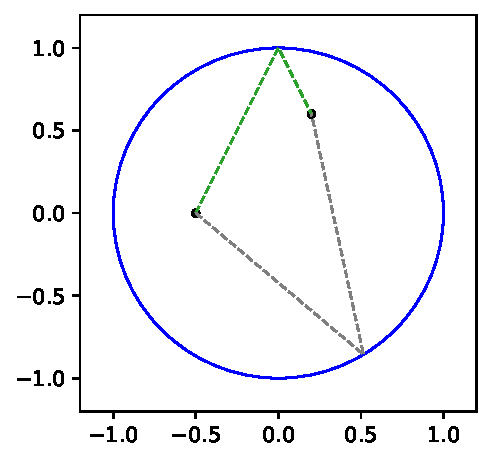
\includegraphics{./ADOneDimManually_files/figure-pdf/fig-billardproblemsolutionwithmathsad-output-1.pdf}

}

\caption{\label{fig-billardproblemsolutionwithmathsad}Lösung des
Billardproblems mit anderen Startwerten.}

\end{figure}

\end{tcolorbox}

\bookmarksetup{startatroot}

\hypertarget{references}{%
\chapter*{References}\label{references}}
\addcontentsline{toc}{chapter}{References}

\hypertarget{refs}{}
\begin{CSLReferences}{1}{0}
\leavevmode\vadjust pre{\hypertarget{ref-Arens2022}{}}%
Arens, Tilo, Frank Hettlich, Christian Karpfinger, Ulrich Kockelkorn,
Klaus Lichtenegger, und Hellmuth Stachel. 2022. \emph{Mathematik}.
Berlin, Heidelberg: Springer Berlin Heidelberg.

\leavevmode\vadjust pre{\hypertarget{ref-Baydin18}{}}%
Baydin, Atilim Gunes, Barak A. Pearlmutter, Alexey Andreyevich Radul,
und Jeffrey Mark Siskind. 2018. {„Automatic Differentiation in Machine
Learning: a Survey``}. \emph{Journal of Machine Learning Research} 18
(153): 1--43. \url{http://jmlr.org/papers/v18/17-468.html}.

\leavevmode\vadjust pre{\hypertarget{ref-Gander1992}{}}%
Gander, Walter. 1992. \emph{Computermathematik}. Birkhäuser.

\leavevmode\vadjust pre{\hypertarget{ref-Gander2015}{}}%
---------. 2015. \emph{Learning {MATLAB}: A Problem Solving Approach}.
1. Aufl. UNITEXT. Cham, Switzerland: Springer International Publishing.

\leavevmode\vadjust pre{\hypertarget{ref-Griewank2008EDP}{}}%
Griewank, Andreas, und Andrea Walther. 2008. \emph{Evaluating
Derivatives: {P}rinciples and Techniques of Algorithmic
Differentiation}. 2nd Aufl. Other Titles in Applied Mathematics 105.
Philadelphia, PA: SIAM. \url{http://bookstore.siam.org/ot105/}.

\leavevmode\vadjust pre{\hypertarget{ref-Henrard2017ADi}{}}%
Henrard, Marc. 2017. \emph{Algorithmic Differentiation in Finance
Explained}. Financial Engineering Explained. Cham: Palgrave Macmillan.
\url{https://doi.org/10.1007/978-3-319-53979-9}.

\leavevmode\vadjust pre{\hypertarget{ref-Hromkovic2021}{}}%
Hromkovic, Juraj, Jarka Arnold, Cédric Donner, Urs Hauser, Matthias
Hauswirth, Tobias Kohn, Dennis Komm, David Maletinsky, und Nicole Roth.
2021. \emph{{INFORMATIK}, Programmieren und Robotik: Grundlagen der
Informatik f{ü}r Schweizer Maturit{ä}tsschulen}.

\leavevmode\vadjust pre{\hypertarget{ref-Slater2022}{}}%
Slater, Max. 2022. {„Differentiable programming from scratch``}. Juli
2022. \url{https://thenumb.at/Autodiff/}.

\leavevmode\vadjust pre{\hypertarget{ref-Weitz2021}{}}%
Weitz, Edmund. 2021. \emph{Konkrete Mathematik (nicht nur) f{ü}r
Informatiker}. 2. Aufl. Wiesbaden, Germany: Springer Spektrum.

\end{CSLReferences}



\end{document}
